%Tech Science Press (CMES)
\documentclass[journal,cmes,article,submit,moreauthors,pdftex]{Definitions/tsp}
%%%%Update on 30 November 2023%%%
\usepackage[normalem]{ulem} % For using the command \uuline{} in the \abstract 
\usepackage{amsfonts} % Use for some special math mark
%%\usepackage{pxfonts} % Use for some special math mark 
%\usepackage{wasysym} % Use for some special mark
%\usepackage{subfigure} % For some paper the use \subfigure
\usepackage{mathcomp} % For permille mark
\usepackage{CJKutf8} % For Chinese font
\usepackage{pifont} % For some special mark 
\usepackage{bm} % Forr math enviroment bold format
\usepackage{bbm} % For some math fancy characters
\graphicspath{{./Definitions/}} % Use for import path the figures paper used

\makeatletter
\def\T@n@@nc@d@ngM@cr@M@d{}
\def\LY@n@@nc@d@ngM@cr@M@d{}
\makeatother

\let\orignewcommand\newcommand  % Store the original \newcommand
\let\newcommand\providecommand  % Make \newcommand behave like \providecommand
\usepackage{verse}
\let\newcommand\orignewcommand  % Use the original `\newcommand` in future
\makeatletter
\renewcommand*{\theHpoemline}{\arabic{verse@envctr}.\arabic{poemline}} % Use the original definition from verse.sty
\makeatother

% Define a matrix envrioment
\newsavebox\foobox
\newcommand{\slantbox}[2][.2]{\mbox{%
        \sbox{\foobox}{#2}%
        \hskip\wd\foobox
        \pdfsave
        \pdfsetmatrix{1 0 #1 1}%
        \llap{\usebox{\foobox}}%
        \pdfrestore
}}

%\setlength{\fboxsep}{0cm}

% Define triangledown mark
\let\oldblacktriangledown\blacktriangledown

% Define italic In, Max
\newcommand{\mmathit}[1]{
  \ifthenelse{\equal{#1}{\ln}}{\mathit{ln}}{
    \ifthenelse{\equal{#1}{\max}}{\mathit{max}}{\mathit{#1}}
  }
}
\makeatother
\robustify{\footnote}

\DeclareUnicodeCharacter{1E45}{\.{n}}
\DeclareUnicodeCharacter{1E41}{\.{m}}
\DeclareUnicodeCharacter{2003}{\quad}
%\DeclareUnicodeCharacter{0177}{\^{y}}
%\DeclareUnicodeCharacter{101}{\={a}}
\DeclareUnicodeCharacter{2009}{\thinspace}
\DeclareUnicodeCharacter{2002}{\enspace{}}
\DeclareUnicodeCharacter{2005}{\thinspace}
\DeclareUnicodeCharacter{0263}{\textipa{G}}
%\DeclareUnicodeCharacter{117}{\.{e}}
\DeclareUnicodeCharacter{A0}{~}
\DeclareUnicodeCharacter{2460}{\textcircled{\scriptsize{1}}}
\DeclareUnicodeCharacter{2461}{\textcircled{\scriptsize{2}}}
\DeclareUnicodeCharacter{2462}{\textcircled{\scriptsize{3}}}
\DeclareUnicodeCharacter{2463}{\textcircled{\scriptsize{4}}}
\DeclareUnicodeCharacter{2464}{\textcircled{\scriptsize{5}}}
\DeclareUnicodeCharacter{2465}{\textcircled{\scriptsize{6}}}
\DeclareUnicodeCharacter{2466}{\textcircled{\scriptsize{7}}}
\DeclareUnicodeCharacter{2467}{\textcircled{\scriptsize{8}}}
\DeclareUnicodeCharacter{2468}{\textcircled{\scriptsize{9}}}
\DeclareUnicodeCharacter{2070}{\textsuperscript{0}}
\DeclareUnicodeCharacter{2074}{\textsuperscript{4}}
\DeclareUnicodeCharacter{2075}{\textsuperscript{5}}
\DeclareUnicodeCharacter{2076}{\textsuperscript{6}}
\DeclareUnicodeCharacter{2077}{\textsuperscript{7}}
\DeclareUnicodeCharacter{2078}{\textsuperscript{8}}
\DeclareUnicodeCharacter{2079}{\textsuperscript{9}}
\DeclareUnicodeCharacter{02C2}{<}
\DeclareUnicodeCharacter{2033}{\relax\ifmmode '' \else $''$\fi}
\DeclareUnicodeCharacter{2034}{\relax\ifmmode ''' \else $'''$\fi}
\DeclareUnicodeCharacter{2026}{\relax\ifmmode … \else $\ldots$\fi}
\DeclareUnicodeCharacter{0229}{\c{e}}
\DeclareUnicodeCharacter{016F}{\r{u}}
%\DeclareUnicodeCharacter{0218}{\cb{S}}
%\DeclareUnicodeCharacter{0219}{\cb{s}}
%\DeclareUnicodeCharacter{021B}{\cb{t}}
\DeclareUnicodeCharacter{127}{\relax\ifmmode\rm\hbar\else $\rm\hbar$\fi}
\DeclareUnicodeCharacter{3AC}{\relax\ifmmode\acute{\alpha}\else $\acute{\alpha}$\fi}
\DeclareUnicodeCharacter{3AD}{\relax\ifmmode\acute{\varepsilon}\else $\acute{\varepsilon}$\fi}
\DeclareUnicodeCharacter{3AE}{\relax\ifmmode\acute{\eta}\else $\acute{\eta}$\fi}
\DeclareUnicodeCharacter{3AF}{\relax\ifmmode\acute{\iota}\else $\acute{\iota}$\fi}
\DeclareUnicodeCharacter{3CC}{\relax\ifmmode\acute{o}\else $\acute{o}$\fi}
\DeclareUnicodeCharacter{3CD}{\relax\ifmmode\acute{\upsilon}\else $\acute{\upsilon}$\fi}
\DeclareUnicodeCharacter{3CE}{\relax\ifmmode\acute{\omega}\else $\acute{\omega}$\fi}
\DeclareUnicodeCharacter{391}{A}
\DeclareUnicodeCharacter{392}{B}
\DeclareUnicodeCharacter{395}{E}
\DeclareUnicodeCharacter{396}{Z}
\DeclareUnicodeCharacter{397}{H}
\DeclareUnicodeCharacter{399}{I}
\DeclareUnicodeCharacter{39A}{K}
\DeclareUnicodeCharacter{39C}{M}
\DeclareUnicodeCharacter{39D}{N}
\DeclareUnicodeCharacter{39F}{O}
\DeclareUnicodeCharacter{3A1}{P}
\DeclareUnicodeCharacter{3A4}{T}
\DeclareUnicodeCharacter{3A7}{X}

\DeclareUnicodeCharacter{27E6}{\relax\ifmmode \llbracket \else $\llbracket$\fi}
\DeclareUnicodeCharacter{27E7}{\relax\ifmmode \rrbracket \else $\rrbracket$\fi}
\DeclareUnicodeCharacter{00B5}{\relax\ifmmode \mu{} \else $\mu$\fi}
\DeclareUnicodeCharacter{1D434}{\relax\ifmmode A \else $A$\fi}
\DeclareUnicodeCharacter{1D435}{\relax\ifmmode B \else $B$\fi}
\DeclareUnicodeCharacter{1D436}{\relax\ifmmode C \else $C$\fi}
\DeclareUnicodeCharacter{1D437}{\relax\ifmmode D \else $D$\fi}
\DeclareUnicodeCharacter{1D438}{\relax\ifmmode E \else $E$\fi}
\DeclareUnicodeCharacter{1D439}{\relax\ifmmode F \else $F$\fi}
\DeclareUnicodeCharacter{1D43A}{\relax\ifmmode G \else $G$\fi}
\DeclareUnicodeCharacter{1D43B}{\relax\ifmmode H \else $H$\fi}
\DeclareUnicodeCharacter{1D43C}{\relax\ifmmode I \else $I$\fi}
\DeclareUnicodeCharacter{1D43D}{\relax\ifmmode J \else $J$\fi}
\DeclareUnicodeCharacter{1D43E}{\relax\ifmmode K \else $K$\fi}
\DeclareUnicodeCharacter{1D43F}{\relax\ifmmode L \else $L$\fi}
\DeclareUnicodeCharacter{1D440}{\relax\ifmmode M \else $M$\fi}
\DeclareUnicodeCharacter{1D441}{\relax\ifmmode N \else $N$\fi}
\DeclareUnicodeCharacter{1D442}{\relax\ifmmode O \else $O$\fi}
\DeclareUnicodeCharacter{1D443}{\relax\ifmmode P \else $P$\fi}
\DeclareUnicodeCharacter{1D444}{\relax\ifmmode Q \else $Q$\fi}
\DeclareUnicodeCharacter{1D445}{\relax\ifmmode R \else $R$\fi}
\DeclareUnicodeCharacter{1D446}{\relax\ifmmode S \else $S$\fi}
\DeclareUnicodeCharacter{1D447}{\relax\ifmmode T \else $T$\fi}
\DeclareUnicodeCharacter{1D448}{\relax\ifmmode U \else $U$\fi}
\DeclareUnicodeCharacter{1D449}{\relax\ifmmode V \else $V$\fi}
\DeclareUnicodeCharacter{1D44A}{\relax\ifmmode W \else $W$\fi}
\DeclareUnicodeCharacter{1D44B}{\relax\ifmmode X \else $X$\fi}
\DeclareUnicodeCharacter{1D44C}{\relax\ifmmode Y \else $Y$\fi}
\DeclareUnicodeCharacter{1D44D}{\relax\ifmmode Z \else $Z$\fi}
\DeclareUnicodeCharacter{1D44E}{\relax\ifmmode a \else $a$\fi}
\DeclareUnicodeCharacter{1D44F}{\relax\ifmmode b \else $b$\fi}
\DeclareUnicodeCharacter{1D450}{\relax\ifmmode c \else $c$\fi}
\DeclareUnicodeCharacter{1D451}{\relax\ifmmode d \else $d$\fi}
\DeclareUnicodeCharacter{1D452}{\relax\ifmmode e \else $e$\fi}
\DeclareUnicodeCharacter{1D453}{\relax\ifmmode f \else $f$\fi}
\DeclareUnicodeCharacter{1D454}{\relax\ifmmode g \else $g$\fi}
\DeclareUnicodeCharacter{1D456}{\relax\ifmmode i \else $i$\fi}
\DeclareUnicodeCharacter{1D457}{\relax\ifmmode j \else $j$\fi}
\DeclareUnicodeCharacter{1D458}{\relax\ifmmode k \else $k$\fi}
\DeclareUnicodeCharacter{1D459}{\relax\ifmmode l \else $l$\fi}
\DeclareUnicodeCharacter{1D45A}{\relax\ifmmode m \else $m$\fi}
\DeclareUnicodeCharacter{1D45B}{\relax\ifmmode n \else $n$\fi}
\DeclareUnicodeCharacter{1D45C}{\relax\ifmmode o \else $o$\fi}
\DeclareUnicodeCharacter{1D45D}{\relax\ifmmode p \else $p$\fi}
\DeclareUnicodeCharacter{1D45E}{\relax\ifmmode q \else $q$\fi}
\DeclareUnicodeCharacter{1D45F}{\relax\ifmmode r \else $r$\fi}
\DeclareUnicodeCharacter{1D460}{\relax\ifmmode s \else $s$\fi}
\DeclareUnicodeCharacter{1D461}{\relax\ifmmode t \else $t$\fi}
\DeclareUnicodeCharacter{1D462}{\relax\ifmmode u \else $u$\fi}
\DeclareUnicodeCharacter{1D463}{\relax\ifmmode v \else $v$\fi}
\DeclareUnicodeCharacter{1D464}{\relax\ifmmode w \else $w$\fi}
\DeclareUnicodeCharacter{1D465}{\relax\ifmmode x \else $x$\fi}
\DeclareUnicodeCharacter{1D466}{\relax\ifmmode y \else $y$\fi}
\DeclareUnicodeCharacter{1D467}{\relax\ifmmode z \else $z$\fi}

\DeclareUnicodeCharacter{1E67}{\.{\v s}}
\DeclareUnicodeCharacter{1E11}{\relax\ifmmode \c{d} \else $\c{d}$\fi}
\DeclareUnicodeCharacter{1ECB}{\relax\ifmmode \d{i} \else $\d{i}$\fi}
\DeclareUnicodeCharacter{1D8D}{\relax\ifmmode \textlhookx \else $\textlhookx$\fi}
\DeclareUnicodeCharacter{104}{\relax\ifmmode \k{A} \else $\k{A}$\fi}
\DeclareUnicodeCharacter{211E}{\relax\ifmmode \textrecipe \else $\textrecipe$\fi}
\DeclareUnicodeCharacter{29D}{\relax\ifmmode \textctj \else $\textctj$\fi}

\DeclareUnicodeCharacter{1E2E}{\'{\"I}}
\DeclareUnicodeCharacter{23F}{\textrts}

\DeclareUnicodeCharacter{2C73}{\varw}

\DeclareUnicodeCharacter{2127}{\mho}

\DeclareUnicodeCharacter{28C}{\textturnv}
\DeclareUnicodeCharacter{252}{\textturnscripta}
\DeclareUnicodeCharacter{259}{\schwa}
\DeclareUnicodeCharacter{25B}{\m{e}}
\DeclareUnicodeCharacter{266}{\m{h}}
\DeclareUnicodeCharacter{127}{\B{h}}
\DeclareUnicodeCharacter{27E}{\textfishhookr}
\DeclareUnicodeCharacter{281}{\textinvscr}



\continuouspages{}
\firstpage{1}
\makeatletter
\setcounter{page}{\@firstpage}
\makeatother
\pubvolume{0}
\issuenum{0}
\elocationid{0}
\articlenumber{0}
\pubyear{2026}
\doiyear{2026}
\copyrightyear{2026}
\datereceived{}
\dateaccepted{}
\dateonlinefirst{}
\datepublished{}

\usepackage{mathtools}
\usepackage{siunitx}
\usepackage{algorithm}
\usepackage{algpseudocode}
\usepackage{booktabs}
\usepackage{multirow}

\newcommand{\R}{\mathbb{R}}
\newcommand{\C}{\mathbb{C}}
\newcommand{\norm}[1]{\lVert #1 \rVert}
\newcommand{\infn}[1]{\lVert #1 \rVert_{\infty}}
\newcommand{\mean}{\operatorname{mean}}
\newcommand{\numv}[1]{#1}
\newcommand{\chimax}{0.50}
\newcommand{\epsbar}{0.03}
\newcommand{\gbnorm}{1.6606}
\newcommand{\betacert}{0.8303}
\newcommand{\NumGammaW}{0.915}
\newcommand{\NumClassOne}{0.4037}
\newcommand{\NumClassBest}{0.4037}
\newcommand{\NumClassBestK}{1}
\newcommand{\NumClassEight}{0.4055}
\newcommand{\NumClassHundred}{0.4055}
\newcommand{\NumConsTwo}{0.3913}
\newcommand{\NumConsBest}{0.3716}
\newcommand{\NumConsBestK}{24}
\newcommand{\NumConsEight}{0.3731}
\newcommand{\NumUncBest}{0.3411}
\newcommand{\NumUncBestK}{8}
\newcommand{\NumUncEight}{0.3411}
\newcommand{\NumPriceDelta}{0.032}
\newcommand{\NumPriceDeltaLo}{0.025}
\newcommand{\NumPriceDeltaHi}{0.032}
\newcommand{\NumPriceBudget}{0.0295}
\newcommand{\NumPriceProjUnc}{0.0067}
\newcommand{\NumPriceProjCons}{0.0109}
\newcommand{\NumFrBaseDsmRreLo}{0.821}
\newcommand{\NumFrBaseDsmRreHi}{0.889}
\newcommand{\NumFrBaseDsmResLo}{0.647}
\newcommand{\NumFrBaseDsmResHi}{0.691}
\newcommand{\NumFrBaseDsmPeakHi}{0.17}
\newcommand{\NumFrBaseBornRreLo}{1.061}
\newcommand{\NumFrBaseBornRreHi}{2.173}
\newcommand{\NumFrBaseBornResHi}{0.779}
\newcommand{\NumFrKernRreLo}{1.035}
\newcommand{\NumFrKernRreHi}{1.092}
\newcommand{\NumFrKernResLo}{0.086}
\newcommand{\NumFrKernResHi}{0.162}
\newcommand{\NumBoxGb}{1.6606}
\newcommand{\NumBoxEdge}{0.6022}
\newcommand{\NumBoxBetaSixty}{0.9964}
\newcommand{\NumBoxBetaEighty}{1.3285}
\newcommand{\NumBoxBetaHundred}{1.6606}
\newcommand{\NumBoxRreConsSixty}{0.3806}
\newcommand{\NumBoxRreConsEighty}{0.3866}
\newcommand{\NumBoxRreConsHundred}{0.3949}
\newcommand{\NumBoxRreUncSixty}{0.3471}
\newcommand{\NumBoxRreUncEighty}{0.3506}
\newcommand{\NumBoxRreUncHundred}{0.3576}
\newcommand{\NumBoxChiConsSixty}{0.600}
\newcommand{\NumBoxChiConsEighty}{0.800}
\newcommand{\NumBoxChiConsHundred}{1.000}
\newcommand{\NumBoxRuns}{6}
\newcommand{\NumDepDeltaArchPct}{-0.56}
\newcommand{\NumDepDeltaUniPct}{0.76}
\newcommand{\NumDepDeltaUncUniPct}{-0.33}
\newcommand{\NumDepUniConsSixteen}{0.36567}
\newcommand{\NumDepUniConsTwentyFour}{0.36846}
\newcommand{\NumDepUniDrift}{\ensuremath{1.1\times10^{-2}}}
\newcommand{\NumDepUniFloor}{\ensuremath{1.8\times10^{-2}}}
\newcommand{\NumDepUniShiftSixteen}{\ensuremath{8.0\times10^{-3}}}
\newcommand{\NumDepUniShiftTwentyFour}{\ensuremath{3.2\times10^{-3}}}
\newcommand{\NumSsimCons}{0.6785}
\newcommand{\NumSsimUnc}{0.7892}
\newcommand{\NumSsimClsEight}{0.3609}
\newcommand{\NumSsimClsFiveZero}{0.3613}
\newcommand{\NumPsnrCons}{17.02}
\newcommand{\NumPsnrUnc}{18.76}
\newcommand{\NumPsnrClsEight}{15.62}
\newcommand{\NumPsnrClsFiveZero}{15.62}
\newcommand{\NumNImg}{4}
\newcommand{\NumRreImgCons}{0.3132}
\newcommand{\NumRreImgUnc}{0.2569}
\newcommand{\NumResConsHead}{0.0529}
\newcommand{\NumResConsEnd}{0.0843}
\newcommand{\NumResConsTrans}{0.1659}
\newcommand{\NumResConsBandLo}{0.0391}
\newcommand{\NumResConsBandHi}{0.1005}
\newcommand{\NumResClsEnd}{0.0003}
\newcommand{\NumSensCons}{0.1617}
\newcommand{\NumSensUnc}{0.1648}
\newcommand{\NumSigMin}{1.132}
\newcommand{\NumSigMax}{5.659}
\newcommand{\NumLipHCons}{0.2503}
\newcommand{\NumLipHUnc}{2.704}
\newcommand{\NumLipRatioUncCons}{10.8}
\newcommand{\NumLipOverEps}{8.3}
\newcommand{\NumGdCompDeltaPct}{+1.2}
\newcommand{\NumPhysWBlock}{0.6176}
\newcommand{\NumSigCompCons}{1.736}
\newcommand{\NumSigCompUnc}{2.247}
\newcommand{\NumSigCompLayerCons}{3.161}
\newcommand{\NumSigCompLayerUnc}{3.111}
\newcommand{\NumResUncSpike}{0.290}
\newcommand{\NumAlphaCons}{0.27--0.31}
\newcommand{\NumAlphaUnc}{0.22--0.31}
\newcommand{\NumGradConsOne}{0.00299}
\newcommand{\NumGradUncOne}{0.104}
\newcommand{\NumEbWorst}{0.01}
\newcommand{\NumEbBest}{0.12}
\newcommand{\NumAblClsProjOn}{0.4094}
\newcommand{\NumAblClsChi}{0.500}
\newcommand{\NumAblProjDelta}{0.028}
\newcommand{\NumMeasChiNoProj}{1.522}
\newcommand{\NumBetaMeas}{2.528}
\newcommand{\NumFrzUncOnShort}{0.3411}
\newcommand{\NumFrzUncOn}{0.4011}
\newcommand{\NumFrzUncOffShort}{5.7228}
\newcommand{\NumFrzUncOff}{\ensuremath{\mathrm{div.}}}
\newcommand{\NumFrzUncBreak}{31}
\newcommand{\NumFrzUncOffChi}{46.948}
\newcommand{\NumFrzConsOnShort}{0.3731}
\newcommand{\NumFrzConsOn}{0.3832}
\newcommand{\NumFrzConsOffShort}{0.4948}
\newcommand{\NumFrzConsOff}{0.5249}
\newcommand{\NumFrzConsOffChi}{0.737}
\newcommand{\NumSeedN}{15}
\newcommand{\NumSeedNCons}{5}
\newcommand{\NumSeedNUnc}{5}
\newcommand{\NumSeedNProjOff}{5}
\newcommand{\NumSeedRreSdCons}{0.0017}
\newcommand{\NumSeedRreSdUnc}{0.0036}
\newcommand{\NumSeedRreMeanCons}{0.3725}
\newcommand{\NumSeedRreMeanUnc}{0.3389}
\newcommand{\NumSeedRreMedCons}{0.3728}
\newcommand{\NumSeedRreMedUnc}{0.3390}
\newcommand{\NumSeedRreHiCons}{0.3739}
\newcommand{\NumSeedRreHiUnc}{0.3422}
\newcommand{\NumSeedExMeanCons}{0.3877}
\newcommand{\NumSeedExMeanUnc}{0.4548}
\newcommand{\NumSeedExSdCons}{0.0020}
\newcommand{\NumSeedExSdUnc}{0.0099}
\newcommand{\NumSeedChiConsMax}{0.50}
\newcommand{\NumSeedProjOffBox}{0.85--1.26}
\newcommand{\NumSeedFinite}{15/15}
\newcommand{\NumRepFloorMaxRre}{0.0181}
\newcommand{\NumRepFloorMedRre}{0.0021}
\newcommand{\NumRepFloorMaxExtrap}{0.0346}
\newcommand{\NumRepNShared}{9}
\newcommand{\NumRepFiniteStable}{yes}
\newcommand{\NumRepBoxStable}{yes}
\newcommand{\NumGdPhysSigma}{3.123}
\newcommand{\NumGdPhysSigmaConv}{1.8437}
\newcommand{\NumSigCompLayerConsConv}{1.8624}
\newcommand{\NumGdPhysSigmaSp}{1.751}
\newcommand{\NumGdRatioSp}{1.784}
\newcommand{\NumGdRatioNcg}{1.693}
\newcommand{\NumGdRatioNet}{1.054}
\newcommand{\NumGdVsPaPct}{0.00}
\newcommand{\NumBjacVsGdPct}{0.00}
\newcommand{\NumChiLipRowCons}{0.553}
\newcommand{\NumChiLipRowFCons}{0.614}
\newcommand{\NumChiFBlockCons}{0.405}
\newcommand{\NumChiRhoFCons}{0.170}
\newcommand{\NumChiRhoFFixCons}{0.022}
\newcommand{\NumChiRhoFFixUnc}{0.020}
\newcommand{\NumChiLipRowUnc}{1.310}
\newcommand{\NumChiLipRowFUnc}{0.785}
\newcommand{\NumChiFBlockUnc}{0.500}
\newcommand{\NumChiRhoFUnc}{0.100}
\newcommand{\NumMJFullCons}{82.45}
\newcommand{\NumMJFullArgmaxM}{8}
\newcommand{\NumMJFullUnc}{650.22}
\newcommand{\NumMJFullArgmaxMUnc}{8}
\newcommand{\NumSigA}{0.912}
\newcommand{\NumSigB}{0.815}
\newcommand{\NumSigC}{1.601}
\newcommand{\NumSigCLower}{1.601}
\newcommand{\NumSigCRatio}{1.0000}
\newcommand{\NumSigLowBound}{1.601}
\newcommand{\NumPhysSigma}{1.845}
\newcommand{\NumThmFieldD}{0.9152}
\newcommand{\NumEColMax}{3.201}
\newcommand{\NumEInfRatio}{2.218}
\newcommand{\NumAlphaC}{0.3124}
\newcommand{\NumInstrErr}{\ensuremath{1.05\times10^{-7}}}
\newcommand{\NumBornSigmaFull}{1.739}
\newcommand{\NumBornSigmaA}{0.500000}
\newcommand{\NumBornSigmaB}{0.000000}
\newcommand{\NumBornSigmaC}{1.600674}
\newcommand{\NumLambdaMeas}{1.175}
\newcommand{\NumLambdaBound}{6770.7}
\newcommand{\NumLamMin}{\ensuremath{9.41\times10^{-6}}}
\newcommand{\NumOpPrecRel}{\ensuremath{1.3\times10^{-7}}}
\newcommand{\NumLayerPrecAmp}{\ensuremath{3.4\times10^{-3}}}
\newcommand{\NumPrecRatioLo}{0.56}
\newcommand{\NumPrecRatioHi}{1.10}
\newcommand{\NumPrecAlphaWorst}{0.500}
\newcommand{\NumSigSingleWorst}{1.75}
\newcommand{\NumSigDoubleWorst}{3.12}
\newcommand{\NumPrecAmp}{\ensuremath{2.6\times10^{4}}}
\newcommand{\NumFSixFourSigErr}{\ensuremath{2.8\times10^{-12}}}
\newcommand{\NumCostLayerOverhead}{0.165}
\newcommand{\NumCostCnnPct}{7.0}
\newcommand{\NumCostCgPct}{69.0}
\newcommand{\NumCostLayerOverheadPct}{16.5}
\newcommand{\NumCostMacOverheadPct}{18.3}
\newcommand{\NumNoiseNominalDb}{300}
\newcommand{\NumNoiseFloorDb}{151.8}
\newcommand{\NumNoiseFloorRel}{\ensuremath{2.57\times10^{-8}}}
\newcommand{\NumAlphaSweepN}{8}
\newcommand{\NumLamCorrTerm}{\ensuremath{1.32\times10^{-3}}}
\newcommand{\NumLamCorrRatio}{\ensuremath{2.0\times10^{-7}}}
\newcommand{\NumTOneRelOn}{\ensuremath{7.47\times10^{-2}}}
\newcommand{\NumTOneRelOff}{\ensuremath{9.32\times10^{-18}}}
\newcommand{\NumWeylRhs}{2.873}
\newcommand{\NumRhoChiCons}{0.467}
\newcommand{\NumRhoChiUnc}{0.971}
\newcommand{\NumRhoChiSpecCons}{0.444}
\newcommand{\NumRhoChiSpecUnc}{0.555}
\newcommand{\NumCgResidImpl}{\ensuremath{2.90\times10^{-4}}}
\newcommand{\NumCgResidConv}{\ensuremath{8.18\times10^{-10}}}
\newcommand{\NumNCgConv}{200}
\newcommand{\NumFdBlockD}{\ensuremath{8.6\times10^{-13}}}
\newcommand{\NumFdBlockAImpl}{0.82}
\newcommand{\NumFdBlockAConv}{\ensuremath{1.79\times10^{-2}}}
\newcommand{\NumDfRelAImplLo}{0.816}
\newcommand{\NumDfRelAImplHi}{1.000}
\newcommand{\NumDfAbsAImplLo}{0.003}
\newcommand{\NumDfAbsAImplHi}{0.015}
\newcommand{\NumDfRelAFine}{1.000}
\newcommand{\NumSigAImpl}{1.175}
\newcommand{\NumSigBImpl}{2.789}
\newcommand{\NumSigmaFullImpl}{3.123}
\newcommand{\NumMJCons}{3.013}
\newcommand{\NumRhoComp}{0.505}
\newcommand{\NumGapRatio}{3.440}
\newcommand{\NumLamRel}{0.05}
\newcommand{\NumNCg}{15}
\newcommand{\NumScaleRes}{2.0}
\newcommand{\NumLipResidChan}{0.0078}
\newcommand{\NumFeatJointLip}{3.03}
\newcommand{\NumdEdChi}{9.787}
\newcommand{\NumGridL}{0.64}
\newcommand{\NumGridFftErr}{\ensuremath{9.7\times10^{-16}}}
\newcommand{\NumGridGbDense}{1.660635}
\newcommand{\NumGridGbLo}{1.6606}
\newcommand{\NumGridGbMd}{1.6536}
\newcommand{\NumGridGbHi}{1.6516}
\newcommand{\NumGridBetaLo}{0.8303}
\newcommand{\NumGridBetaMd}{0.8268}
\newcommand{\NumGridBetaHi}{0.8258}
\newcommand{\NumGridELo}{3.295}
\newcommand{\NumGridEMd}{3.312}
\newcommand{\NumGridEHi}{3.318}
\newcommand{\NumGridAlphaCLo}{0.3035}
\newcommand{\NumGridAlphaCHi}{0.3014}
\newcommand{\NumGridGsLo}{0.0883}
\newcommand{\NumGridGsHi}{0.0221}
\newcommand{\NumGridDriftGbPct}{0.55}
\newcommand{\NumGridDriftEPct}{0.70}
\newcommand{\NumGridFactor}{16}
\newcommand{\NumCgRatio}{40}
\newcommand{\NumCgNMin}{5}
\newcommand{\NumCgNMax}{200}
\newcommand{\NumCgCMin}{0.8480}
\newcommand{\NumCgCMax}{0.8480}
\newcommand{\NumCgDMin}{0.7935}
\newcommand{\NumCgDMax}{0.7935}
\newcommand{\NumCgAMin}{0.723}
\newcommand{\NumCgAMax}{0.874}
\newcommand{\NumCgBMin}{0.118}
\newcommand{\NumCgBMax}{3.515}
\newcommand{\NumCgFullMin}{0.7368}
\newcommand{\NumCgFullMax}{3.6769}
\newcommand{\NumCgFullFaithLo}{1.2043}
\newcommand{\NumCgFullFaithHi}{1.9791}
\newcommand{\NumCgCFlatPct}{0.00}
\newcommand{\NumCgDFlatPct}{0.00}
\newcommand{\NumCgRImplImpl}{0.3718}
\newcommand{\NumCgRImplConv}{0.3575}
\newcommand{\NumCgRConvImpl}{0.3914}
\newcommand{\NumCgRConvConv}{0.3769}
\newcommand{\NumCgRImplTen}{0.3821}
\newcommand{\NumCgRConvTen}{0.4019}
\newcommand{\NumCgLossImpl}{0.00854}
\newcommand{\NumCgLossConv}{0.01139}
\newcommand{\NumCgLossRatio}{1.3}
\newcommand{\NumBornInitRre}{0.4876}
\newcommand{\NumCsiSecHundred}{305.4}
\newcommand{\NumSomSecHundred}{14.8}
\newcommand{\NumCsiBest}{0.3671}
\newcommand{\NumCsiBestK}{100}
\newcommand{\NumCsiAtKEight}{0.4121}
\newcommand{\NumSomBest}{0.3160}
\newcommand{\NumSomBestK}{100}
\newcommand{\NumSomBestM}{20}
\newcommand{\NumSomMGrid}{6, 12, 20}
\newcommand{\NumSomAtKEight}{0.3706}
\newcommand{\NumSomAtKEightM}{20}
\newcommand{\NumSomMargKEight}{-0.0025}
\newcommand{\NumSomMargBest}{-0.0557}
\newcommand{\NumBetaZeroFive}{0.8286}
\newcommand{\NumRreZeroFive}{0.3731}
\newcommand{\NumMaxWZeroFive}{0.6757}
\newcommand{\NumCycGainZeroFive}{5.1}
\newcommand{\NumSensZeroFive}{0.162}
\newcommand{\NumBetaSevenFive}{1.2420}
\newcommand{\NumRreSevenFive}{0.4131}
\newcommand{\NumMaxWSevenFive}{0.7071}
\newcommand{\NumCycGainSevenFive}{9.4}
\newcommand{\NumFracBoxSevenFive}{0.211}
\newcommand{\NumBetaOneZero}{1.6555}
\newcommand{\NumRreOneZero}{0.4858}
\newcommand{\NumMaxWOneZero}{0.7178}
\newcommand{\NumCycGainOneZero}{6.7}
\newcommand{\NumProjOffChiOneZero}{1.4}
\newcommand{\NumProjOffWOneZero}{1.774}
\newcommand{\NumFracBoxOneZero}{0.256}
\newcommand{\NumBetaOneFive}{2.4824}
\newcommand{\NumRreOneFive}{0.6092}
\newcommand{\NumMaxWOneFive}{0.7229}
\newcommand{\NumCycGainOneFive}{33.6}
\newcommand{\NumProjOffChiOneFive}{2.2}
\newcommand{\NumProjOffWOneFive}{2.980}
\newcommand{\NumFracBoxOneFive}{0.291}
\newcommand{\NumSensOneFive}{0.199}
\newcommand{\NumMaxChiBox}{0.50}
\newcommand{\NumFieldSubCertZeroFive}{0.6762}
\newcommand{\NumFieldSubCertSevenFive}{0.7479}
\newcommand{\NumFieldSubCertOneZero}{0.7727}
\newcommand{\NumFieldSubCertOneFive}{0.7848}
\newcommand{\NumBetaGeomEll}{0.8286}
\newcommand{\NumRreRectEll}{0.4263}
\newcommand{\NumRreEllEll}{0.3731}
\newcommand{\NumMaxWGeomEll}{0.672}
\newcommand{\NumBetaGeomRect}{0.8293}
\newcommand{\NumRreRectRect}{0.3877}
\newcommand{\NumRreEllRect}{0.4333}
\newcommand{\NumMaxWGeomRect}{0.643}
\newcommand{\NumBetaGeomStripe}{0.8295}
\newcommand{\NumRreRectStripe}{0.4790}
\newcommand{\NumRreEllStripe}{0.5028}
\newcommand{\NumMaxWGeomStripe}{0.665}
\newcommand{\NumBetaGeomBlob}{0.8302}
\newcommand{\NumRreRectBlob}{0.5014}
\newcommand{\NumRreEllBlob}{0.5353}
\newcommand{\NumMaxWGeomBlob}{0.643}
\newcommand{\NumFresnelFreq}{2.0}
\newcommand{\NumFresnelLamCm}{14.99}
\newcommand{\NumFresnelChiMax}{2.0}
\newcommand{\NumFresnelRadiusCm}{1.5}
\newcommand{\NumFresnelEpsR}{3.0}
\newcommand{\NumFresnelDomainLam}{3.0}
\newcommand{\NumFresnelGb}{7.1994}
\newcommand{\NumFresnelBeta}{14.3987}
\newcommand{\NumFresnelBetaAtHalf}{3.5997}
\newcommand{\NumFresnelBetaRatio}{17.34}
\newcommand{\NumFresnelGbRatio}{4.34}
\newcommand{\NumFresnelSigmaLBSynth}{1.648}
\newcommand{\NumFresnelPubRsM}{0.72}
\newcommand{\NumFresnelPubRrM}{0.76}
\newcommand{\NumFresnelPubNinc}{36}
\newcommand{\NumFresnelPubNrx}{49}
\newcommand{\NumFresnelPubGs}{0.1791}
\newcommand{\NumFresnelPubEpeak}{5.051}
\newcommand{\NumFresnelPubAlphaC}{0.1980}
\newcommand{\NumFresnelPubSigmaLB}{2.525}
\newcommand{\NumAblUncPOnFbOnRre}{0.4061}
\newcommand{\NumAblUncPOnFbOnChi}{0.500}
\newcommand{\NumBetaUncPOnFbOn}{0.830}
\newcommand{\NumAblUncPOnFbOffRre}{0.3988}
\newcommand{\NumAblUncPOnFbOffChi}{0.500}
\newcommand{\NumBetaUncPOnFbOff}{0.830}
\newcommand{\NumAblUncPOffFbOnRre}{0.3779}
\newcommand{\NumAblUncPOffFbOnChi}{1.522}
\newcommand{\NumBetaUncPOffFbOn}{2.528}
\newcommand{\NumAblUncPOffFbOffRre}{0.3775}
\newcommand{\NumAblUncPOffFbOffChi}{1.422}
\newcommand{\NumBetaUncPOffFbOff}{2.362}
\newcommand{\NumAblConsPOnFbOnRre}{0.3848}
\newcommand{\NumAblConsPOnFbOnChi}{0.500}
\newcommand{\NumBetaConsPOnFbOn}{0.830}
\newcommand{\NumAblConsPOnFbOffRre}{0.3853}
\newcommand{\NumAblConsPOnFbOffChi}{0.500}
\newcommand{\NumBetaConsPOnFbOff}{0.830}
\newcommand{\NumAblConsPOffFbOnRre}{0.3963}
\newcommand{\NumAblConsPOffFbOnChi}{0.726}
\newcommand{\NumBetaConsPOffFbOn}{1.206}
\newcommand{\NumAblConsPOffFbOffRre}{0.3969}
\newcommand{\NumAblConsPOffFbOffChi}{0.727}
\newcommand{\NumBetaConsPOffFbOff}{1.208}
\newcommand{\NumClsSweepKEight}{1.0 / 0.4055}
\newcommand{\NumClsSweepKTwoFour}{0.3 / 0.4054}
\newcommand{\NumClsSweepKFifty}{0.5 / 0.4055}
\newcommand{\NumClsSweepKHundred}{0.8 / 0.4054}
\newcommand{\NumClsSweepBest}{0.8 / 0.4054}
\newcommand{\NumClsSweepBestK}{K=100}
\newcommand{\NumClsSweepGain}{\ensuremath{1.4\times10^{-5}}}


\graphicspath{{figures/}}

\newcommand{\orcidauthorA}{0009-0008-1394-7953}

\Title{Fixed Points and Certified Boundedness of Unrolled Born/Contrast-Source Inverse Scattering Networks}

\Author{Longgang Wang\textsuperscript{1,*}\orcidA, Guoqiang Wang\textsuperscript{1}, and Nianfeng Shi\textsuperscript{1}}
\AuthorNames{Longgang Wang, Guoqiang Wang and Nianfeng Shi}

\address{%
\textsuperscript{1}Luoyang Institute of Science and Technology, Luoyang 471000, Henan, China
}

\corres{Corresponding Author: Longgang Wang. Email: longgangwang@163.com}

\abstract{Unrolled networks for electromagnetic inverse scattering replace classical Born or contrast-source iterations by a cascade in which a physical update is followed by a small learned correction. Whether the trained composite map retains any convergence property of the iteration it unrolls is usually left open. This paper answers it for the Born/contrast-source family. A layer is a fixed-point map on the (contrast, contrast-source) state. The Jacobian block mapping contrast perturbations into the contrast-source channel is exactly a scaled diagonal of the total field, so its largest singular value is closed-form. This yields a step-size threshold above which no correction acting on the contrast channel can make the implemented layer Euclidean-contractive, whatever its Lipschitz constant. Certification is therefore layered: we prove field-subsystem contraction and an invariant compact set for the full rollout under a nonexpansive contrast projection, and give an exact finite-depth noise account that keeps the non-normal correction the geometric bound omits, whose hypothesis fails here. At the operating point the composite layer reaches $\sigma_{\max}=\numv{\NumPhysSigma}$ while the field subsystem contracts ($\beta_0=\numv{\betacert}$), and the weak-scattering condition holds only inside the certified contrast box. Ablations over 800 unrolled layers isolate the projection as the ingredient that guarantees boundedness; the operator-level certificates are recomputed on a published Fresnel geometry, where the weak-scattering condition fails while the non-contractivity bound tightens, and a reconstruction from measured scattered fields is reported for nine phantom-frequency pairs, without the trained weights. The framework delivers certified boundedness and layer-wise error accounting under stated conditions, rather than an unconditional convergence guarantee.}

\keyword{inverse scattering; deep unrolling; fixed-point iteration; contraction mappings; spectral normalization; convergence of learning systems; Lippmann--Schwinger equation}

\makeatletter
\setlength{\@fptop}{0pt}
\setlength{\@fpsep}{14pt plus 3pt}
\setlength{\@fpbot}{0pt plus 1fil}
\makeatother
\renewcommand{\topfraction}{0.92}
\renewcommand{\bottomfraction}{0.65}
\renewcommand{\textfraction}{0.06}
\renewcommand{\floatpagefraction}{0.78}

\begin{document}

\section{Introduction}
Electromagnetic inverse scattering problems (ISPs) require reconstructing the spatial contrast of
an unknown region from scattered near- or far-field measurements. The underlying
Lippmann--Schwinger equation is nonlinear, because of multiple scattering, and ill-posed, so every
classical solver trades accuracy against iteration count and regularization: the Born and
distorted-Born iterative methods \cite{born_lit}, contrast-source inversion (CSI) \cite{csi_lit}
and the subspace optimization method (SOM) \cite{som_lit}.

A now-established line of work \emph{unrolls} these iterations into deep networks: each layer
implements one modified iteration and a small learned module corrects it. Representative
instances are SOM-Net \cite{somnet}, the unrolled CSI/ResNet architecture of Zhang \emph{et al.}
\cite{unrolledcnn}, the Neural Born Iterative Method (NeuralBIM) \cite{neuralbim}, the DeepNIS
cascade \cite{deepnis} and its multi-frequency extension \cite{mfneuralbim}, the
contraction-integral-equation unrolling of Xu \emph{et al.} \cite{ciesomnet}, and the kernelized
unfolding of Li \emph{et al.} \cite{kernelunroll}. Li \emph{et al.} \cite{li2019cnn} analysed the
layer-count dynamics of the DeepNIS cascade. Each of these papers reports a gain over its
classical ancestor at a fixed computational budget. Those claims belong to those papers and are
not re-established here. Our own comparison is narrower: it is an \emph{iteration-count} comparison against one classical baseline at
matched per-layer cost, and we state the residual per-layer cost difference alongside the numbers,
together with the fact that the comparison is in iterations and not in wall-clock time.

They also share a structural weakness: \emph{no operator-level convergence guarantee for the trained composite map}. Some prior work reports empirical stability or layer-count behaviour, but none states a per-layer sufficient condition, a fixed-point characterisation, or an error bound for the full unrolled Born/contrast-source map after training. The learned updates are free
to break the contraction properties that make the original iteration meaningful. Consequently,
(i) increasing depth beyond the trained value can degrade or destabilize the output;
(ii) the sensitivity of the output to measurement noise is uncontrolled; and (iii) the fixed
point of the learned iteration, what the network computes if layers are repeated, may
drift arbitrarily far from the solution of the physical equation the network claims to solve.
For linear sparse coding this tension is well understood: LISTA-type analyses
\cite{lista, listacp, alista} prove linear convergence by \emph{constraining} the learnable
weights, a partial weight coupling, and iterative-regularization analyses of unfolded proximal
schemes \cite{cui_reg} establish stability for convex inverse problems. Monotone-operator and
nonexpansive architectures \cite{sherry_nonexp, mondeq} provide existence and uniqueness
guarantees for implicit layers. None of these tools applies directly to the nonlinear,
non-self-adjoint operators of scattering theory. Layer-level operator-level guarantees for the
trained unrolled Born/contrast-source map are, to our knowledge, not yet stated in the literature.

\emph{Contribution.} For the Born/contrast-source class of unrolled ISPs we provide the missing
theory, meet the obstruction head-on, and make the result operational:
\begin{enumerate}
\item \textbf{Layer-level operator form.} The discrete
Lippmann--Schwinger system is written as a fixed-point iteration of a physics operator
$T^{\mathrm{phys}}$ on the state $z=(\chi,w)$, with $\chi$ the contrast and $w$ the contrast source; the contrast step is
the regularized least-squares solve of the data equation, not a single preconditioned gradient step,
so that the operator we analyse differs from the classical schemes by a \emph{solved} system rather
than by one gradient step. The implementation evaluates that solve by a fixed
$n_{\mathrm{cg}}=\numv{\NumNCg}$-step conjugate-gradient loop, so we distinguish throughout between
the exact least-squares \emph{map}, the symbolic object analysed, and the truncated solver
\emph{actually run}: the two certified blocks below are solver-free, and the solver-dependent
contrast-path blocks are reported at both resolutions. An unrolled network is exactly a cascade of layers
$T_k = (1-\theta_k)I+\theta_k T^{\mathrm{phys}}_{\alpha_k,\gamma_k} + H_k$ with $H_k$ a learned
correction and $\theta_k$ an explicit relaxation, and its fixed points are characterized exactly by Prop.~\ref{prop:fixpoint}.
\item \textbf{Impossibility of per-layer (Euclidean) contraction, in threshold form.} For the faithful
composite the $w^{+}$-with-respect-to-$\chi$ block of the layer Jacobian is \emph{exactly}
$\theta\alpha\,\mathrm{diag}(E)$. Reading off its largest singular value
$\sigma_{\max}(J)$, which is the Euclidean Lipschitz constant of the block, gives the rigorous
$\alpha$-explicit bound $\sigma_{\max}(J)\ge\theta\alpha\mathcal{E}$, hence a provable
non-contractivity threshold $\alpha_c=(\theta\mathcal{E})^{-1}$ rather than a
margin claimed to be independent of $\alpha$. That block is shared by the full layer Jacobian: the correction and the projection leave the field channel alone, so the same bound holds
\emph{with} the learned correction, for any Lipschitz constant; we also record why the natural
perturbation route through Weyl's inequality cannot be used to obtain it. We additionally show that linearising the contrast
step (the Born variant) leaves this bound unchanged, so the obstruction originates in the bilinear
coupling of the \emph{field} step and is a property of the architecture, not of the data-misfit
nonlinearity. Below $\alpha_c$ the bound is inconclusive, and we report the measured
$\sigma_{\max}(\alpha)$ over a grid, with proved and measured statements kept separate.
\item \textbf{Layer-wise certification instead of per-layer contraction.}
We prove what \emph{is} available: an a-priori field-subsystem contraction
$\beta_0=\chi_{\max}\norm{\mathbf{G}_b}_2=\numv{\betacert}<1$ that holds for every step size by Thm.~\ref{thm:field}; a certified invariant compact set for the whole rollout under a
nonexpansive physics-prior projection by Thm.~\ref{thm:bounded}; an \emph{exact} finite-depth noise
accounting together with the non-normal correction factor $\kappa_2(V)$ that the naive
geometric bound $\Lambda/(1-\rho)$, with $\rho$ the spectral radius, omits, as
Prop.~\ref{prop:noise} and Cors.~\ref{cor:noisegeo}--\ref{cor:noisenormal} show,
and, separately, the measured transient $M_J:=\sup_{1\le m\le K}\norm{J^m}$ that a naive
reading would substitute for that factor,
together with a proof that the substitution is invalid, Remark~\ref{rem:mj};
an explicit constructive bound on the data-Lipschitz constant $\Lambda$ of \eqref{eq:Lambda}; and a conditional drift radius $\bar\epsilon/(1-\rho_\chi)$ for
infinite-depth extrapolation under Cor.~\ref{cor:fidelity}, where
$\rho_\chi$ is the global Lipschitz constant of $F$ on the compact set, i.e.\ $\sup_{\chi\in B}\norm{DF(\chi)}_2<1$, which is stronger than a pointwise spectral radius condition. The two geometric statements are
\emph{conditional}. The per-layer contraction-rate hypothesis
($\rho<1$, Cor.~\ref{cor:noisegeo}) is not satisfied at the measured operating point
($\sigma_{\max}(J)=\numv{\NumPhysSigma}>1$), and the drift radius of
Cor.~\ref{cor:fidelity} is reported as conditional; the $K{=}8$ composite's spectral radius
$\rho=\numv{\NumRhoComp}<1$ is a separate quantity that must not be conflated with the layer
$\sigma_{\max}$ of a non-normal map.

These certificates are additionally recomputed at the operator level on the published
Institut Fresnel 2-D geometry, where the weak-scattering condition fails while the
non-contractivity bound tightens, and a reconstruction from measured fields on the published
dielectric phantoms is reported for nine phantom-frequency pairs without the trained correction
weights.

\item \textbf{The price of certification, measured.} Ablations over $800$
unrolled layers isolate which ingredient delivers which guarantee. Removing the projection from frozen weights makes the unconstrained network
explode ($\infn{\chi}$ from $\numv{\chimax}$ to $\numv{\NumFrzUncOffChi}$); retraining without it
restores empirical boundedness but pushes the measured contrast bound past the weak-scattering
threshold ($\beta_0^{\mathrm{meas}}=\numv{\NumBetaMeas}>1$), so \emph{no a-priori certificate
survives}. The amplitude budget buys the a-priori constants at a measurable accuracy cost of
$\numv{\NumPriceDelta}$; the spectral clamp alone produces no observed stability gain, because the
per-layer composite gain is governed by the coupling block $\theta\alpha\,\mathrm{diag}(E)$ rather
than by the correction, and the physics core is non-contractive on its own
($\numv{\NumPhysSigma}>1$ at the converged contrast solve). A third ablation shows that bounding the
correction trunk's input is what keeps the \emph{state} inside the admissible box: without it the
contrast leaves the box ($\infn{\chi}=\numv{\NumAblUncPOffFbOffChi}$) while the reconstruction error
stays finite, so a finite error is not evidence that the certificate holds.
\end{enumerate}
Taken together, the results replace the informal claim ``unrolled inverse scattering works'' by an
explicit list of what can be certified, what cannot, and what each design choice costs.

\section{Related Work}\label{sec:related}
\subsection{Deep unrolling for inverse scattering}
SOM-Net \cite{somnet} unrolls SOM with learned network modules; Zhang \emph{et al.}
\cite{unrolledcnn} embed CSI iterations into a ResNet-type unrolled structure; NeuralBIM
\cite{neuralbim} learns the alternating residual updates of the Born iterative method with
independent CNNs, in supervised and unsupervised variants; a multi-frequency extension appeared
in \cite{mfneuralbim}; CIE-SOM-NET \cite{ciesomnet} reduces nonlinearity through a contraction
integral equation and reports improved stability; \cite{kernelunroll} adds kernelized physical
constraints. All of these works validate performance empirically; to our knowledge none of them
supplies a layer-level sufficient condition, a fixed-point characterisation or an error bound for
the trained iteration, and the omission matters, because the property that would have to be
assumed is exactly the one the learned modules are free to break. The word ``contraction'' in
\cite{ciesomnet} refers to a property of the physical integral equation used to \emph{model} the
scattering, not to a convergence analysis of the learned iteration; no sufficient condition, no
fixed-point characterization and no error bound for the trained network is given. Our analysis
acts at the layer level and is therefore complementary, but its scope is narrower than the list
above. For architectures whose physics kernel is the Born/contrast-source composite analysed
here, it applies as soon as the learned modules satisfy the two budgets of the
constrained scheme. For architectures with a \emph{different} physics kernel, the
subspace-based SOM-Net \cite{somnet}, or the compressed-integral-equation CIE-SOM-NET
\cite{ciesomnet}, what transfers is the \emph{template}, namely certify the rollout layer by
layer from one closed-form block and one CG-free field block, not the certificates themselves:
$C=\theta\alpha\,\mathrm{diag}(E)$ and the field recursion of Thm.~\ref{thm:field} are properties
of the contrast-source step and have to be re-derived for another kernel; our guarantees are
therefore stated for the Born/contrast-source composite analysed here and are not extrapolated to
other physics kernels.

\subsection{Convergence theory of unrolled networks}
For linear sparse coding, Chen \emph{et al.} \cite{listacp} prove linear convergence of LISTA
\cite{lista} under a partial coupling of the learnable weights, a condition later simplified by
ALISTA \cite{alista}; Tay \cite{algomapping} treats a different mapping at every iteration. Cui
\emph{et al.} \cite{cui_reg} prove stability of unfolded proximal gradients under learned convex
penalties. Spectral-norm constraints give nonexpansive networks by design \cite{sherry_nonexp},
monotone-operator equilibrium networks guarantee existence and uniqueness of equilibria for
implicit layers \cite{mondeq}, and Mukherjee \emph{et al.} \cite{mukherjee2023} survey the
convergence guarantees available for learned reconstruction. These results cover
linear measurement operators, convex penalties, or implicit infinite-depth models. The composite
studied here is neither: the physics core is an affine map in the field variable whose coefficients
depend bilinearly on the contrast, and it is not the gradient of any functional that the scheme
minimizes. That mismatch is not a technical inconvenience but an impossibility. Two neighbouring literatures are \emph{not} invoked here, because their
hypotheses do not transfer: convergence analyses of non-convex unrolled proximal/ADMM schemes
assume a convex data term and read the layer as a proximal step, and plug-and-play /
regularization-by-denoising analyses assume the proximal operator of an explicit regularizer.
Neither reading is available for the Born/contrast-source composite, which is not the gradient of
any functional the scheme minimizes.

\subsection{Learned iterative reconstruction in imaging}
Beyond scattering, unrolling is used in MRI and computational imaging, as the surveys of Monga
\emph{et al.} \cite{monga_survey} and Cui \emph{et al.} \cite{cui_reg} describe; the general lesson,
that learned iterations need constrained parameterizations to retain guarantees, carries over, but the scattering operator's
non-normality and the absence of a gradient-descent interpretation of the
Born/CSI scheme require the dedicated treatment developed below.

Table~\ref{tab:guarantees} condenses the comparison the way the guarantees themselves
are stated, family by family.

\begin{table}[htbp]
\centering
\caption{Guarantee landscape. For each family we list the property that is
\emph{actually proved}, the operator or setting it applies to, and what transfers to the
Born/contrast-source composite analysed here. ``None'' marks families that report no
formal guarantee for the trained iteration.}
\label{tab:guarantees}
\small\setlength{\emergencystretch}{1.5em}\hfuzz=0.75pt
\renewcommand{\arraystretch}{1.2}
\begin{tabular}{@{}p{0.19\textwidth}p{0.24\textwidth}p{0.18\textwidth}p{0.30\textwidth}@{}}
\toprule
Method / family & Property proved & Setting it applies to & Relation to this work \\
\midrule
SOM-Net \cite{somnet}, kernelised SOM \cite{kernelunroll} & None (empirical) &
subspace-based SOM kernel & the \emph{template} transfers (certify the rollout from a
closed-form block plus a CG-free field block); the certificates
$C=\theta\alpha\,\mathrm{diag}(E)$ do not \\
Unrolled CNN \cite{unrolledcnn}, NeuralBIM \cite{neuralbim,mfneuralbim} & None (empirical) &
CSI / Born-iterative kernel & \emph{same} kernel family: the per-layer impossibility and
the certificates apply once the two budgets of the constrained scheme hold \\
CIE-SOM-NET \cite{ciesomnet} & contraction of the \emph{physical} integral equation &
compressed-integral-equation kernel & ``contraction'' refers to the model, not to a
guarantee for the trained iteration; template only \\
LISTA-CP \cite{listacp}, ALISTA \cite{alista}, per-mapping analysis \cite{algomapping} &
linear convergence under weight coupling & linear sparse coding (linear measurement map) &
hypotheses do not transfer: the scattering core is bilinear in $(\chi,w)$ \\
Iterative regularisation \cite{cui_reg} & stability of unfolded proximal gradients &
convex learned penalties & no proximal or variational reading of the Born--CSI step \\
Nonexpansive by design \cite{sherry_nonexp} & nonexpansiveness from a spectral-norm budget &
generic Lipschitz networks & yields no fixed point and no error bound for the bilinear map \\
MonDEQ \cite{mondeq} & existence and uniqueness of equilibria & implicit layers with a
monotone operator & the composite is non-monotone; a different certificate is required \\
Classical CSI / SOM / Born \cite{csi_lit,som_lit,born_lit,convergentborn} &
convergence of the \emph{unlearned} iteration (e.g.\ $\chi_{\max}\norm{G_b}_2<1$) &
iteration without a learned module & supplies the classical $\beta_0<1$; we add the
layer-level impossibility and the certificate for the \emph{learned} iteration \\
\textbf{This work} & per-layer Euclidean non-contraction; certified field-subsystem
contraction, boundedness and fidelity & Born/contrast-source kernel & n/a \\
\bottomrule
\end{tabular}
\end{table}

The claim is deliberately narrower than ``a convergence guarantee for unrolled inverse
scattering'', and we separate it into three tiers so that a reader can tell what is borrowed,
what is new, and what is only evidence.
\emph{Borrowed:} the weak-scattering condition $\beta_0<1$ and the Neumann-series argument behind
it, the nonexpansiveness of an interval projection, the Banach fixed-point theorem, and the
elementary block structure of a damped alternating scheme.
\emph{New, theoretical:} the exact coupling block $C=\theta\alpha\,\mathrm{diag}(E)$ of the
contrast-to-contrast-source channel, and the fact that the implemented layer shares that whole row,
so a step-size threshold above which no correction confined to the contrast channel can restore a
contractive layer follows without any hypothesis on that correction's Lipschitz constant; the
separation of field-subsystem contraction, boundedness of the rollout and convergence of the
composite map into three statements with different hypotheses, only the first two of which are
proved; a closed-form invariant set that does not involve the learned correction at all; and an
exact finite-depth noise recursion whose hypotheses we check and, for the geometric form, find
false here.
\emph{New, evidential:} the numerical audit of the blocks against their closed forms, the
truncation sweep that shows which quantities survive a change of solver, the projection ablation
that separates boundedness by construction from boundedness observed in one trained parameter
set, and the operator-level recomputation on a published measured geometry.
We claim no priority for the observation that unrolled networks in general lack convergence
guarantees, which is well documented, and none of the three tiers asserts a guarantee that the
hypotheses do not cover.

\section{Problem Formulation and Operator Form}\label{sec:form}
\subsection{Scalar 2-D TM scattering and its MoM discretization}
Let $D$ be a bounded domain in $\R^2$ with background wavenumber $k_b=k_0\sqrt{\varepsilon_b}$,
and let $\chi(r)=\varepsilon_r(r)-\varepsilon_b$ denote the contrast (with a free-space background,
so $\varepsilon_b=1$ and $\chi=\varepsilon_r-1$, giving $\varepsilon_r\in[1.25,1.5]$ for the
$\chi\in[0.25,0.5]$ range studied). For a TM incident field the
total field obeys the Lippmann--Schwinger equation
\begin{equation}\label{eq:ls}
E(r) = E^{i}(r) + k_b^2\!\int_D G(r,r')\,\chi(r')\,E(r')\,\mathrm{d}r',
\end{equation}
with $G(r,r')=-\tfrac{j}{4}H_0^{(2)}(k_b|r-r'|)$. Discretizing \eqref{eq:ls} by pulse basis
functions and point collocation over $n$ cells gives, per incidence $i$,
\begin{equation}\label{eq:discrete}
w = \chi\odot\big(E^i + \mathbf{G}_b w\big),\qquad
y = \mathbf{G}_s w + n,
\end{equation}
where $w_i=\chi\odot E_i$ is the contrast source, $\mathbf{G}_b=k_b^2\Delta A\,
[G(r_m,r'_l)]$ is the (discretely singular) electric-field integral operator on $D$, and
$\mathbf{G}_s$ maps $D$ to the $n_{\mathrm{rx}}$ receivers. Stacking the $n_{\mathrm{inc}}$
incidences, let $z=(\chi,w)\in\R^n\times\C^{n\times n_{\mathrm{inc}}}$ and write
$\norm{\cdot}$ for the Euclidean norm on the realified state
$(\chi,\mathrm{Re}\,w,\mathrm{Im}\,w)$. All matrix and operator norms below are the
induced spectral norms unless stated otherwise.

Writing the system as \eqref{eq:discrete}, a contrast source that is a \emph{local} function of $\chi$ and the field, and therefore cheap to evaluate, together with a linear data equation, is itself
classical: it is the starting point of contrast source inversion \cite{csi_lit}, and the same
rewriting is what makes the contraction-integral-equation family reformulate the problem so that
the implicit part is carried by a better-conditioned operator \cite{cie_lit}. The state
$z=(\chi,w)$ and the alternation below are therefore not a modelling choice of ours; what we
add is the analysis of what a \emph{learned} perturbation of this alternation can and cannot
preserve.

\subsection{The physical iteration}
Classical Born/contrast-source schemes alternate a \emph{field step} (solve \eqref{eq:discrete}
for $w$ given $\chi$) and a \emph{contrast step} (update $\chi$ from the data equation given
$E$). We use the damped/regularized form
\begin{align}
w^{+} &= (1-\alpha)w+\alpha\,\chi\odot\big(E^{i}+\mathbf{G}_b w\big),
\label{eq:fieldstep}\\
E &= E^{i}+\mathbf{G}_b w^{+},
\label{eq:Estep}\\
\hat\chi^{\mathrm{LS}}(E;y) &= \arg\min_{\chi\in\R^{n}}\big\|\mathbf{G}_s\mathrm{diag}(E)\chi-y\big\|_F^{2}+\sum_{j=1}^{n}\lambda_j\chi_j^{2},
\label{eq:contraststep}\\
\chi^{+} &= (1-\gamma)\chi+\gamma\,\hat\chi^{\mathrm{LS}}(E;y),
\label{eq:chiupd}
\end{align}
where $\alpha\in(0,1]$ is a field damping factor, $\gamma\in(0,1]$ relaxes the contrast step, and
the Tikhonov weights are diagonally scaled,
$\lambda_j=\lambda_{\mathrm{rel}}\sum_i|E_{ij}|^{2}\norm{\mathbf{G}_s(\cdot,j)}_2^{2}$ with
$\lambda_{\mathrm{rel}}=\numv{\NumLamRel}$. Equation~\eqref{eq:contraststep} is a linear
least-squares problem; the implementation solves it inside every layer by a fixed
$n_{\mathrm{cg}}=\numv{\NumNCg}$ conjugate-gradient steps on its normal equations
(Algorithm~\ref{alg:layer}, step 4), reaching a relative residual of $\numv{\NumCgResidImpl}$. It is
therefore the algebraic solve of the data equation for the current field, \emph{not} a single
preconditioned gradient step, with which it shares its fixed points but not its Jacobian, evaluated
\emph{at a finite truncation}. All symbolic statements below refer to the exact least-squares
\emph{map} \eqref{eq:contraststep}; the solver-resolution effect on the contrast-path
blocks is quantified numerically, and the two certified blocks of Lemma~\ref{lem:blocks} are
free of it. Since $E$ enters \eqref{eq:contraststep} only
through the intermediate $w^{+}$, the least-squares contrast $\hat\chi^{\mathrm{LS}}$ has
\emph{no direct dependence} on $\chi$: its
Jacobian with respect to $\chi$ is nonzero only via the field chain
$\chi\to w^{+}\to E$, a distinction that fixes the block structure in Lemma~\ref{lem:blocks}.
The relaxed update $\chi^{t}=(1-\gamma)\chi+\gamma\hat\chi^{\mathrm{LS}}$ does carry the direct term $(1-\gamma)\chi$, which is the $(1-\theta\gamma)I$ block of $A$ in Lemma~\ref{lem:blocks}.
Equations \eqref{eq:fieldstep}--\eqref{eq:contraststep} define the \emph{physics operator}
$T^{\mathrm{phys}}_{\alpha,\gamma}: z=(\chi,w)\mapsto(\chi^{+},w^{+})$.

\begin{Proposition}[Fixed points of the exact, unprojected physics map]\label{prop:fixpoint}
$z^\star$ is a fixed point of $T^{\mathrm{phys}}_{\alpha,\gamma}$ with $\alpha,\gamma>0$ if and
only if $(\chi^\star,w^\star)$ solves the discrete field equation \eqref{eq:discrete} together with
the normal equations of the regularized data misfit, i.e. $\chi^\star$ is the exact algebraic
least-squares solution of the data equation for the self-consistent field.
\end{Proposition}
\begin{proof}
At a fixed point, \eqref{eq:fieldstep} gives $w^\star=\chi^\star\odot(E^i+\mathbf{G}_bw^\star)$
, which is the field equation, and \eqref{eq:contraststep}--\eqref{eq:layer-code} give $\chi^\star=
\hat\chi^{\mathrm{LS}}(E^\star;y)$, whose stationarity condition is exactly the normal equations
$\mathrm{Re}\sum_i \overline{E^\star_i}\odot\mathbf{G}_s^{H}\big(\mathbf{G}_s(\chi^\star\odot
E^\star_i)-y_i\big)+\lambda\odot\chi^\star=0$. Conversely both stationary conditions give
$z^+=z$.
\end{proof}
The proposition is an algebraic property of the \emph{physics core}: it says which equations the
fixed point of the exact, unprojected map satisfies, and it is not a convergence statement about a
trained network. Neither the truncated solve nor the learned correction preserves it, and no
certificate below is derived from it (Remark~\ref{rem:fixpointtrunc}).
\begin{Remark}[Fixed points of the truncated solver]\label{rem:fixpointtrunc}
Proposition~\ref{prop:fixpoint} characterises the fixed points of the map carrying the \emph{exact}
least-squares solve. The layer actually run truncates that solve at $n_{\mathrm{cg}}$ steps, so its
fixed points satisfy the normal equations only to within the solver residual
($\numv{\NumCgResidImpl}$ here); the field equation, by contrast, is exact, because the field step
contains no iterative solve. The proposition also describes the \emph{unprojected} map; the deployed
layer applies $\Pi_{[0,\chi_{\max}]}$ to the contrast output, so at a boundary cell the projected
fixed point satisfies the constrained optimality condition rather than the unconstrained normal
equation, and the physical fixed point lies in the certified compact set only when it is feasible
($\chi^\star\in[0,\chi_{\max}]$). Nothing certified below leans on the fixed-point characterisation:
the non-contractivity bound rests on the closed-form coupling block $C$, and the boundedness
certificate on the field block $D$ in Lem.~\ref{lem:blocks}; both are independent of the
solver resolution.
\end{Remark}

\subsection{Unrolled network}
A $K$-layer unrolled network is
\begin{equation}\label{eq:layer-code}
z^{k+1} = z^{k}+\theta_k\big(T^{\mathrm{phys}}_{\alpha_k,\gamma_k}(z^{k})-z^{k}\big)+\big(H_k(z^{k};y),\,0\big),
\end{equation}
where $H_k$ is a small CNN acting on the $\chi$ channel, fed with the adjoint-projected data residual, the current fields and the contrast, $\alpha_k,\gamma_k$ are
learnable scalars, and $\theta_k\in(0,1]$ is an explicit \emph{global relaxation} applied to the
physics core only. We declare $\theta_k$ because it is present in the implementation and is easily
left implicit: it leaves fixed points untouched, and on the field channel it is \emph{exactly} the
damping substitution $\alpha_k\mapsto\theta_k\alpha_k$ in \eqref{eq:fieldstep}, which is the
substitution under which Theorem~\ref{thm:bounded} covers it. On the contrast channel it scales the
relaxation of the $\chi$ update by $\theta_k$ but is \emph{not} a pure parameter substitution,
because the field entering the contrast solve is still the $\alpha_k$-damped one; that channel is
controlled by the projection instead, as in Theorem~\ref{thm:bounded}. All experiments reported
here use $\theta_k\equiv1$. The physics core is \emph{not learned} in the sense that its functional
form is \eqref{eq:fieldstep}--\eqref{eq:contraststep}, fixed by the discretization; only the
relaxation scalars and the correction are trained, which anchors the network to \eqref{eq:discrete}.

Algorithm~\ref{alg:layer} states the layer map of \eqref{eq:layer-code} as implemented, so that
every quantity the theory below constrains can be read off the same procedure that produced the
measurements; in particular the contrast step is the solved system \eqref{eq:contraststep}, not a
single preconditioned gradient step, and the projection $\Pi$ is the last operation of the layer.
Freezing the trained scalars at $\alpha_k=\gamma_k=\theta=1$ recovers the classical damped
alternating iteration, so the same procedure covers both.

\begin{algorithm}[t]
\caption{One unrolled layer $T_k$ of \eqref{eq:layer-code}: physics core
$T^{\mathrm{phys}}_{\alpha_k,\gamma_k}$ followed by the learned correction $H_k$.}
\label{alg:layer}
\begin{algorithmic}[1]
\Require $\chi_k$, $w_k$, data $y$, operators $\mathbf{G}_b,\mathbf{G}_s$, field $E^i$
\Require $U_k$, $a_\theta[k]$, $g_\theta[k]$;
constants $\theta$, $\bar\epsilon$, $\chi_{\max}$, $\lambda_{\mathrm{rel}}$, $n_{\mathrm{cg}}$
\State $\alpha_k\gets a_{\max}\varsigma(a_\theta[k])$,
       $\gamma_k\gets g_{\max}\varsigma(g_\theta[k])$
\State $w_t\gets(1-\alpha_k)w_k+\alpha_k\,\chi_k\odot\big(E^i+\mathbf{G}_b w_k\big)$
       \Comment{field update}
\State $E_k\gets E^i+\mathbf{G}_b w_t$
\State $\hat\chi_k\gets\arg\min_{\chi}\norm{y-\mathbf{G}_s\operatorname{diag}(E_k)\chi}_2^2+\sum_j\lambda_j\chi_j^2$
       \Comment{contrast solve}
\State $\chi_t\gets(1-\gamma_k)\chi_k+\gamma_k\hat\chi_k$
\If{$U_k\neq\emptyset$}
  \State $r_k\gets\mathbf{G}_s w_t-y$
  \State $f_k\gets\operatorname{cat}\big(\operatorname{Re},\operatorname{Im}\mathbf{G}_s^{H}r_k;\
         \operatorname{Re},\operatorname{Im}E_k;\
         \operatorname{Re},\operatorname{Im}w_t;\
         \chi_k\big)$
  \State $\Delta\chi_k\gets \bar\epsilon\,\tanh\!\big(U_k(f_k/s)\big)$
         \Comment{learned correction}
\Else
  \State $\Delta\chi_k\gets 0$
\EndIf
\State $\chi_{k+1}\gets \Pi\big(\chi_k+\theta(\chi_t-\chi_k)+\Delta\chi_k\big)$
\State $w_{k+1}\gets w_k+\theta(w_t-w_k)$
\State \Return $(\chi_{k+1},w_{k+1})$
\end{algorithmic}
\end{algorithm}
The regularizer in the contrast step is
$\lambda_j=\lambda_{\mathrm{rel}}\big(\sum_i|E_{ij}|^2\big)\norm{\mathbf{G}_s(\cdot,j)}_2^2$, and
the minimisation is carried out by $n_{\mathrm{cg}}$ conjugate-gradient steps on the normal
equations, i.e.\ as an exact algebraic solve of \eqref{eq:contraststep} rather than as an
approximate subproblem. The per-channel scales $s$ in the correction bound
$\operatorname{Lip}(U_k(\cdot/s))=O(1)$; $\bar\epsilon$ is the amplitude budget of
\eqref{eq:budgets}.

Figure~\ref{fig:structure} summarises the layer. Of its two state channels, the field step
produces $E$ and passes it to the contrast step; the correction $H_k$ acts on the contrast channel
just before the projection $\Pi$; the field channel carries neither. The block map on the right is
the asymmetry this produces: only the field row is common to the core $J$ and to the implemented
layer $DT_k$, which is why the bounds that survive the correction are the ones on $C$ and $D$.

\begin{figure}[htbp]
\centering
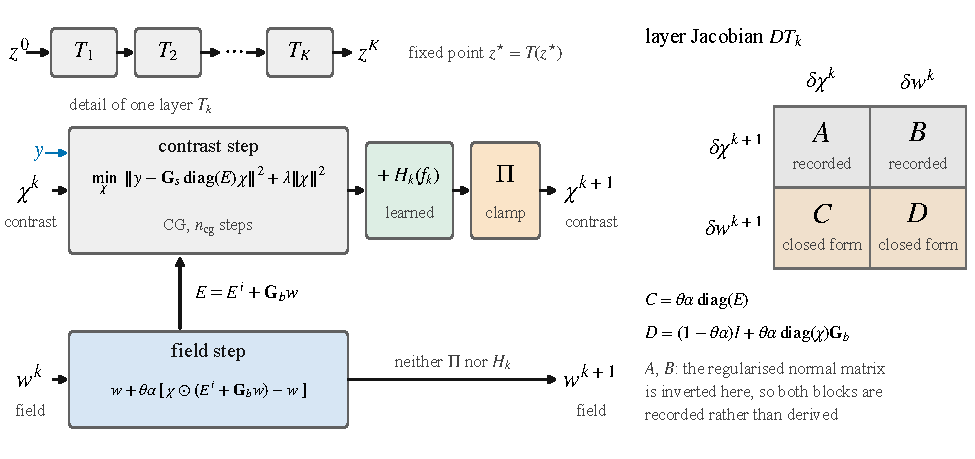
\includegraphics[width=\linewidth]{figures/fig_structure.pdf}
\caption{One unrolled layer and its Jacobian. Top: the unrolled cascade, whose limit point
satisfies $z^{\star}=T(z^{\star})$. Lower left: the two state channels of a single
layer. Right: block map of the layer Jacobian in $(\delta\chi,\delta w)$, rows being the
channels that leave the layer and columns those that enter it.}
\label{fig:structure}
\end{figure}

\section{Convergence Theory}\label{sec:theory}
Figure~\ref{fig:structure} fixes the object analysed in this section: one unrolled layer, its
two update paths, and the four Jacobian blocks that Lemma~\ref{lem:blocks} evaluates exactly.

\emph{Three properties, and which of them are proved.} The results below are frequently read as
if they were one statement about ``the network'', so we separate them once, here, and the rest of
the paper keeps the separation. They concern different maps and none of them implies the next:
\emph{(C) contraction of the field subsystem} at frozen contrast is a property of one affine
update in one channel; \emph{(B) invariance of an explicit compact set} is a property of the
rollout, and it needs the contrast projection; \emph{(F) convergence} is a property of the
complete composite map and would require a unique attracting fixed point. Table~\ref{tab:hierarchy}
records the hypotheses, what each result establishes, and what it explicitly does not.
Throughout, $J$ denotes the Jacobian of the \emph{relaxed physics core} with the learned
correction removed and the projection indicator evaluated at the core argument, and $DT_k$ the
Jacobian of layer $k$ \emph{as implemented}, differentiated through the actual computation
including the truncated CG solve and the projection applied to the composite argument; the two
share the second block row and nothing else, as Lemma~\ref{lem:blocks} makes exact.

\begin{table}[htbp]
\centering
\caption{Guarantee hierarchy. Each row is a statement about a different map and the last column is
the part that is not claimed; the first three rows are proved, the fourth is not.}
\label{tab:hierarchy}
\small
\begin{tabular}{@{}p{0.17\linewidth}p{0.24\linewidth}p{0.26\linewidth}p{0.24\linewidth}@{}}
\toprule
property & object & established when & not established \\
\midrule
(C) field contraction & $w\mapsto(1-\alpha)w+\alpha\chi\odot(E^i+\mathbf{G}_bw)$ at frozen $\chi$
& $\beta_0<1$, all $\alpha\in(0,1]$, rate $1-\alpha(1-\beta_0)$ (Thm.~\ref{thm:field})
& anything about the composite layer or about $\chi$ \\
(B) bounded rollout & full state $(\chi,w)$ under $K$ layers
& projection every layer, $\beta_0<1$, $\inf_k\theta_k\alpha_k>0$ (Thm.~\ref{thm:bounded})
& existence, uniqueness or attraction of a fixed point \\
non-contractivity & one full layer, $DT_k$ & $\alpha>\alpha_c$, any correction on the contrast
channel (Prop.~\ref{prop:imposs}) & that the layer \emph{is} contractive below $\alpha_c$ \\
(F) convergence & repeated composite $T^K$
& not proved here; would need $\rho_\chi<1$, which is measured and not verified
& global convergence, a unique fixed point, or an unconditional noise gain \\
\bottomrule
\end{tabular}
\end{table}

Throughout, $B\subset\R^n\times\C^{n\times n_{\mathrm{inc}}}$ is the invariant compact set supplied
by Theorem~\ref{thm:bounded}; it contains the physical fixed point whenever the projection is
active, and all constants below are defined on $B$. We use
\begin{equation}\label{eq:budgets}
\bar\epsilon := \sup_{k}\sup_{z\in B}\norm{H_k(z;y)},\qquad
\ell := \sup_k \operatorname{Lip}\big(H_k(\cdot;y)\big),
\end{equation}
and, for the admissible-contrast bound $\chi_{\max}$,
\begin{equation}\label{eq:beta0}
\beta_0 \;:=\; \chi_{\max}\,\norm{\mathbf{G}_b}_2 .
\end{equation}
The condition $\beta_0<1$ is \emph{not} a contribution of this paper: it is the classical
convergence condition of the Neumann series for \eqref{eq:ls} in the operator-norm sense \cite{born_lit},
and it has been known since the origins of the subject that the series is only guaranteed to
converge on that side of the threshold, and it can be pushed past that threshold only by modifying the
series, as Kleinman and van den Berg \cite{kleinvandenberg} and Kleinman \emph{et al.}
\cite{convergentborn} show; the weak-scattering validity limits of the
first-order approximation that follow from it are likewise classical \cite{slaney}.
What is new here is only its role as the hypothesis of a \emph{certificate for the unrolled
rollout} of Thm.~\ref{thm:field}, together with the measurement
$\beta_0^{\mathrm{meas}}=\numv{\NumBetaMeas}>1$. Two operating points must be kept apart here,
and the manuscript keeps them apart throughout: the hypothesis \emph{fails} for the arm
retrained without the projection, whose contrast leaves the certified box
($\infn{\chi}=\numv{\NumAblUncPOffFbOnChi}$), whereas
at the certified contrast box $\chi_{\max}=\numv{\chimax}$ the same constant is
$\beta_0=\numv{\betacert}<1$ and the hypothesis \emph{holds} by Thm.~\ref{thm:field}. The
measured value quoted in this paragraph refers to the first of the two, and the certified value
of Thm.~\ref{thm:field} to the second; they are not in conflict.
For non-normal operators $\sigma_{\max}$ and $\rho$ differ, and that difference, not an
oversight, is what makes some of the statements below conditional; where it does, we say so
explicitly and report the measured quantity.

\subsection{Why per-layer Euclidean contraction is impossible}
The obstruction is read off from the block structure of the layer Jacobian, which we record first.

\begin{Lemma}[Exact block structure]\label{lem:blocks}
Let $J=\left[\begin{smallmatrix}A&B\\ C&D\end{smallmatrix}\right]$ be the realified Jacobian at
$z=(\chi,w)$, in the state ordering
$(\chi,\mathrm{Re}\,w,\mathrm{Im}\,w)$, of the \emph{relaxed physics core} of
\eqref{eq:layer-code}, that is, of
$\chi^{+}=\mathbf{1}_{\Pi}[(1-\theta\gamma)\chi+\theta\gamma\,\hat\chi^{\mathrm{LS}}(\chi,w)]$
and $w^{+}=(1-\theta\alpha)w+\theta\alpha\,\chi\odot(E^{i}+\mathbf{G}_b w)$, \emph{with the
learned correction $H_k$ excluded}. The full layer Jacobian $DT_k$ is \emph{not} $J+DH_k$, and the gap matters. As Algorithm~\ref{alg:layer} shows, $\Pi$ is applied to the
\emph{composite} argument $a_{\mathrm{core}}+H_k$, where
$a_{\mathrm{core}}:=\chi+\theta(\chi^{t}-\chi)$, whereas $J$ differentiates the core with the
projection indicator evaluated at $a_{\mathrm{core}}$ alone. Hence
\begin{equation}\label{eq:dTvsJ}
DT_k-J=\Big(\mathbf{1}_{\Pi}^{(a_{\mathrm{core}}+H_k)}-\mathbf{1}_{\Pi}^{(a_{\mathrm{core}})}\Big)M_{\mathrm{core}}+\mathbf{1}_{\Pi}^{(a_{\mathrm{core}}+H_k)}\frac{\partial H_k}{\partial z},
\end{equation}
with $M_{\mathrm{core}}:=\partial a_{\mathrm{core}}/\partial z$ and
$\mathbf{1}_{\Pi}^{(\cdot)}$ the diagonal $0/1$ indicator of the active branch of $\Pi$ at the
stated argument. Both sides are written for the $\chi$-output block row: $M_{\mathrm{core}}$ is
$n\times(n+2nn_{\mathrm{inc}})$, each indicator is $n\times n$ and multiplies it on the left, and
$\partial H_k/\partial z$ is $n\times(n+2nn_{\mathrm{inc}})$, so the products are conformable in
that order and all three terms are $n\times(n+2nn_{\mathrm{inc}})$; the $w$-output rows of $DT_k$
and $J$ coincide, so the corresponding rows of the difference are exactly zero. When the projection is inactive the first term, the projection-indicator difference, vanishes and the gap reduces to the second, $\partial H_k/\partial z$, which is bounded
by $\operatorname{Lip}(H_k)$; the term that $\operatorname{Lip}(H_k)$ does \emph{not} control is the
first one, the projection-indicator difference, which can be as large as $\norm{M_{\mathrm{core}}}$
when $H_k$ pushes a cell across the clamp bound. The interval projector $\Pi_{[0,\chi_{\max}]}$ is non-differentiable at the boundary; the block decomposition below uses the active-branch indicator $\mathbf{1}_{\Pi}$, which is the classical right-derivative convention, and the certified blocks $C$ and $D$ do not touch the contrast projection at all, so the non-differentiability does not affect the impossibility certificate. What \emph{is} exact for both operators
is the second block row: the field update $w^{+}=w+\theta(w_t-w)$ is neither projected nor
corrected, so it contributes the same $C$ and $D$ to $J$ and to $DT_k$ alike. Then, with
$E=E^i+\mathbf{G}_b w\in\C^{n_{\mathrm{inc}}\times n}$
the total field at $z$,
\begin{equation}\label{eq:blocks}
C \;=\; \theta\,\alpha\,\mathrm{diag}(E),\qquad
D \;=\; (1-\theta\alpha)I+\theta\alpha\,\mathrm{diag}(\chi)\,\mathbf{G}_b ,
\end{equation}
while $A=\mathbf{1}_{\Pi}\big[(1-\theta\gamma)I+\theta\gamma\,
\partial\hat\chi^{\mathrm{LS}}/\partial\chi\big]$ and
$B=\theta\gamma\,\partial\hat\chi^{\mathrm{LS}}/\partial w$, both with $\mathbf{1}_{\Pi}$
evaluated at $a_{\mathrm{core}}$: these two are the $\chi$-blocks of the \emph{core}, not of
$DT_k$. The bounds that do carry over to $DT_k$ are therefore those on the common second row,
$C$ and $D$.
\end{Lemma}
\begin{proof}
In the state ordering, $w^{+}$ depends on $\chi$ only through the diagonal factor
$\chi\odot(E^i+\mathbf{G}_b w)$, whose derivative with respect to $\chi$ is
$\mathrm{diag}(E^i+\mathbf{G}_b w)$; the relaxation in \eqref{eq:layer-code} multiplies it by
$\theta\alpha$, giving $C$. The $w$-block follows from
$\partial w^{+}/\partial w=I+\theta\alpha(\mathrm{diag}(\chi)\mathbf{G}_b-I)$, giving $D$. The
$\chi$-block of the core is $\chi^{t}=(1-\gamma)\chi+\gamma\hat\chi^{\mathrm{LS}}$, and
$\hat\chi^{\mathrm{LS}}$ depends on $\chi$ only through $w^{+}$, as Sec.~\ref{sec:form} states, which yields
$A$ and $B$; the projection contributes the $0/1$ factor $\mathbf{1}_{\Pi}$ at
$a_{\mathrm{core}}$ and is otherwise nonexpansive. Differentiating the layer \emph{as
implemented}, the projection applied to $a_{\mathrm{core}}+H_k$, with $H_k$ itself
differentiated inside it, instead gives \eqref{eq:dTvsJ}. The two sides of the additivity identity
$DT_k=J+DH_k$ coincide exactly when $\Pi$ is inactive or switched off, which the off-diagonal
residual confirms directly: it is \numv{\NumTOneRelOff} with the projection off against
\numv{\NumTOneRelOn} with it on, both relative to $\norm{DT_kv}$.
\end{proof}
Two remarks on $C$ are needed for the next proposition, because it is easy to quote its norm
incorrectly. First, the operator in \eqref{eq:blocks} acts on the \emph{spatial} contrast block and
produces an \emph{incidence-stacked} field block: it is a direct sum over cells $r$ of the rank-one
map $\delta\chi_r\mapsto\theta\alpha E_{\cdot,r}\,\delta\chi_r$, where $E_{\cdot,r}\in\C^{n_{\mathrm{inc}}}$
is the $r$-th column of $E$. Its singular values are therefore
$\theta\alpha\norm{E_{\cdot,r}}_2$, $r=1,\dots,n$, with $\norm{\cdot}_2$ taken \emph{along the
incidence axis}. Second, the field $\ell_\infty$ norm $\max_r|E(r)|$ is a
different object and satisfies
$\max_r|E(r)|\le\max_r\norm{E_{\cdot,r}}_2\le\sqrt{n_{\mathrm{inc}}}\,\max_r|E(r)|$; in our
discretization the two differ by a factor of $\numv{\NumEInfRatio}$. Every norm statement below is
made with the column norm
\begin{equation}\label{eq:Ecol}
\mathcal{E}\;:=\;\max_{r}\norm{E_{\cdot,r}}_2 ,
\end{equation}
which is the largest per-cell field energy across incidences.

\begin{Proposition}[Impossibility of composite contraction: threshold form]\label{prop:imposs}
All norms below are the equal-weighted Euclidean norm on the real state
$(\chi,\operatorname{Re}w,\operatorname{Im}w)$. The bound is therefore coordinate-dependent: a
linear rescaling of the field variable rescales the coupling block $C$, and with it the threshold
$\alpha_c=(\theta\mathcal{E})^{-1}$, so the impossibility is a statement about this metric, not an
architecture-invariant fact. The rescaling does not weaken the statement: it re-expresses the same
physical map in another norm, and the threshold moves with the norm; what survives every
equal-weight choice is the existence of step sizes, namely those above $\alpha_c$ in the chosen
metric, on which no contrast-channel correction restores a contractive layer. With that
convention, for every $\alpha,\gamma\in(0,1]$ and every
$z\in B$, the layer Jacobian satisfies the three \emph{rigorous} lower bounds
\begin{equation}\label{eq:impossbound}
\sigma_{\max}(J)\;\ge\;\underbrace{\theta\alpha\,\mathcal{E}}_{\sigma_{\max}(C)}\;,
\qquad
\sigma_{\max}(J)\;\ge\;\sigma_{\max}(B)\;,\qquad
\sigma_{\max}(J)\;\ge\;\sigma_{\max}(A),
\end{equation}
the first with an explicit closed form because $C$ is a direct sum of rank-one blocks, as Lem.~\ref{lem:blocks} shows. Hence the layer map is provably non-contractive on the whole step-size
range
\begin{equation}\label{eq:alphac}
\alpha>\alpha_c:=(\theta\,\mathcal{E})^{-1},
\end{equation}
i.e.\ $\sigma_{\max}(J)>1$ there, and $\alpha_c$ decreases as the peak field column norm
$\mathcal{E}$ grows. Moreover the \emph{full} layer Jacobian inherits the first bound with no
auxiliary hypothesis: since the second block row is common to $J$ and $DT_k$ by Lem.~\ref{lem:blocks}, a unit test vector supported on the contrast-input block gives
\begin{equation}\label{eq:imposscomp}
\sigma_{\max}(DT_k)\;\ge\;\sigma_{\max}(C)=\theta\alpha\,\mathcal{E}>1
\qquad(\alpha>\alpha_c),
\end{equation}
for \emph{every} correction $H_k$ confined to the contrast channel (so the shared
$\chi\!\to\!w$ block $C$ is unchanged) and every Lipschitz constant $\ell$. On that step-size range no
such correction restores $\sigma_{\max}(DT_k)<1$: the obstruction acts in the
$\chi\!\to\!w$ channel, which a correction applied to the contrast alone cannot reach. The
threshold is a \emph{sufficient} condition for non-contractivity and not a necessary one: above
$\alpha_c$ non-contractivity is proved for every admissible correction, below it the lower bound
in \eqref{eq:impossbound} no longer exceeds one and the question is settled numerically at the
operating points reported in the experimental section.
\end{Proposition}
\begin{proof}
All three bounds are instances of the same elementary fact: for a test vector supported on a single
block, $\sigma_{\max}(J)\ge\norm{J(v,0)}$ or $\ge\norm{J(0,u)}$, and
$J(v,0)=(Av,Cv)$ while $J(0,u)=(Bu,Du)$. Taking $v$ to be the leading right singular vector of $C$
gives $\norm{J(v,0)}\ge\norm{Cv}=\sigma_{\max}(C)$; taking $u$ to be the leading right singular
vector of $B$ gives $\norm{J(0,u)}\ge\sigma_{\max}(B)$; taking $v$ to be the leading right singular
vector of $A$ gives $\sigma_{\max}(J)\ge\sigma_{\max}(A)$ from the same identity. For the first
bound in closed form: $C$ is a direct sum over cells of the rank-one maps
$\delta\chi_r\mapsto\theta\alpha E_{\cdot,r}\delta\chi_r$ of Lem.~\ref{lem:blocks}, whose singular
values are $\theta\alpha\norm{E_{\cdot,r}}_2$; the largest is $\theta\alpha\mathcal{E}$ and is
attained at $v=e_{r^\star}$ with $r^\star=\arg\max_r\norm{E_{\cdot,r}}_2$. The direction matters: an \emph{arbitrary} unit $v$ gives only
$\norm{Cv}\ge\theta\alpha\min_r\norm{E_{\cdot,r}}_2\norm{v}$, and it is the $\ell_\infty$ version
$\max_r|E(r)|$ that would be wrong by the factor discussed under \eqref{eq:Ecol}.
Equation~\eqref{eq:alphac} rearranges $\theta\alpha\mathcal{E}>1$. Finally, $C$ is a block of
$DT_k$ as well as of $J$ by Lem.~\ref{lem:blocks} for any correction that leaves the $\chi\!\to\!w$
block unchanged, so the same test-vector argument yields
\eqref{eq:imposscomp} without invoking \eqref{eq:dTvsJ} and without any hypothesis on such an $H_k$;
a correction acting on the $w$-channel could in principle modify $C$ and is not covered by the
statement.
\end{proof}

\begin{Remark}[Weyl perturbation route]\label{rem:weyl}
Weyl's inequality applied to the additive splitting $DT_k=J+DH_k$ would give
$\sigma_{\max}(DT_k)\ge\sigma_{\max}(J)-\operatorname{Lip}(H_k)$. That splitting is precisely what
\eqref{eq:dTvsJ} rules out, so the inequality is not applicable here and we do not invoke it.
The three quantities in the comparison are nevertheless reported, because they come from
\emph{one} audit run on \emph{one} state, the constrained arm at
the learned step sizes and the implemented $n_{\mathrm{cg}}$, so that the comparison is well
posed in the first place:
$\sigma_{\max}(J)=\numv{\NumGdPhysSigma}$,
$\operatorname{Lip}(H_k)=\numv{\NumLipHCons}$, hence the Weyl lower bound
$\sigma_{\max}(J)-\operatorname{Lip}(H_k)=\numv{\NumWeylRhs}$, while the measured per-layer
composite is $\numv{\NumSigCompLayerCons}$. With the corrected operator these two numbers satisfy
the bound rather than violate it: $\numv{\NumWeylRhs}\le\numv{\NumSigCompLayerCons}$, so Weyl's
inequality is met and there is no numerical contradiction to read off. The reason the perturbation
route still does not yield \eqref{eq:imposscomp} is therefore \emph{structural}, not numerical:
\eqref{eq:dTvsJ} rules out the additive splitting $DT_k=J+DH_k$ because the projection acts on the
composite argument, so the coupling block of $DT_k$ is not $J$'s coupling block plus a correction's;
this holds independently of the magnitudes above. Consequently the block argument of
Prop.~\ref{prop:imposs} is not a stronger variant of the perturbation bound but the only
applicable one: it needs no splitting of $DT_k$ at all, because the coupling block $C$ is shared
by $J$ and by $DT_k$ alike. The numbers are retained so that a reader who reaches for the
perturbation route can verify that the Weyl lower bound is met, and see why the splitting it would
require is nonetheless structurally unavailable. A direct numerical check reproduces the block
structure and the exactness of the shared second row, with relative error zero in double precision,
and confirms the projection on/off control.
\end{Remark}

Four points fix the interpretation. \emph{(a) The margin depends on $\alpha$.} The certified margin
is $\kappa(\alpha)=\theta\alpha\mathcal{E}-1>0$ on $\alpha>\alpha_c$ and it vanishes as
$\alpha\downarrow\alpha_c$; no $\alpha$-independent margin follows from
\eqref{eq:impossbound}, and we make no such claim. The only $\alpha$-uniform lower bound the block
structure supports directly is the weaker envelope
$\sigma_{\max}(J(\alpha))\ge1-\theta\alpha(1+\beta_0)$, obtained from
$\sigma_{\max}(J)\ge\sigma_{\min}(D)\ge1-\theta\alpha(1+\beta_0)$, where
$\sigma_{\min}(D)$ is the smallest singular value of the direct block $D$. \emph{(b) The bound is stated
per operating point and evaluated numerically.} $\mathcal{E}$, $\sigma_{\max}(A)$ and
$\sigma_{\max}(B)$ depend on $z$; we therefore report them at the operating points actually reached,
in the experimental section, rather than as $z$-independent constants, and we state the $\alpha$
dependence explicitly rather than folding it into a single number. The threshold
$\alpha_c=(\theta\mathcal{E})^{-1}$ further inherits the field normalisation: with the incident field
scaled to unit peak, $\mathcal{E}=\max_r\|E_{\cdot,r}\|_2$ scales with the number of illuminations as
$\sqrt{n_{\mathrm{inc}}}$, so comparisons of $\alpha_c$ across configurations must be read together
with their $n_{\mathrm{inc}}$ and normalisation, not as pure architecture statements. \emph{(c) Below $\alpha_c$ the
bound is inconclusive, so we measure.} For $\alpha\le\alpha_c$ nothing follows from
\eqref{eq:impossbound}; the experimental section reports the measured
$\sigma_{\max}(J(\alpha))$ on a grid $\alpha\in[0.05,1]$, marking on which side of $\alpha_c$ each
point lies. \emph{(d) The obstruction is bilinear, not an artefact of the data-misfit
nonlinearity.} Replacing the self-consistent field in the contrast step by the fixed incident field
$E^i$, the Born variant, for which $B\equiv0$ by Lem.~\ref{lem:blocks}, leaves $C$ untouched
($\sigma_{\max}(C)=\numv{\NumBornSigmaC}$, identical to the faithful value $\numv{\NumSigCLower}$),
and the measured composite remains above one ($\numv{\NumBornSigmaFull}$, Table~\ref{tab:cert}).
That variant also has two analytically transparent blocks: because its contrast step no longer
depends on the field state, $\sigma_{\max}(B)\equiv0$ and $\sigma_{\max}(A)=1-\gamma$ exactly, wherever the projection is inactive at the operating point. The instrument reproduces both to
machine precision ($\numv{\NumBornSigmaA}$ and $\numv{\NumBornSigmaB}$), a third exact
self-check, independent of the closed form for $C$. The non-contractivity is therefore created by
the bilinear coupling $\chi\odot E$ in the \emph{field} step and cannot be removed by linearizing
the data misfit.

Proposition~\ref{prop:imposs} is a statement about \emph{architecture}, not about training: on
$\alpha>\alpha_c$ the natural sufficient condition used throughout the unrolling literature, a
Euclidean-contractive layer map, is unavailable for faithful Born/contrast-source networks,
for any correction confined to the contrast channel subject to the coordinate and channel qualifications stated in the proposition. Certification must therefore be \emph{layered}.

\subsection{What can be certified: field subsystem, boundedness, fidelity}
Figure~\ref{fig:regime} locates the two regimes of this section in one plane; they are not
exclusive, and the overlap is the substance of the paper rather than a gap in it. At the
synthetic operating point one has simultaneously $\beta_0=\numv{\betacert}<1$, so the
\emph{field subsystem} is contractive by Thm.~\ref{thm:field}, and
$\alpha>\alpha_c=\numv{\NumAlphaC}$, so the \emph{composite layer} is provably
non-contractive by Prop.~\ref{prop:imposs}.

\begin{figure}[htbp]
\centering
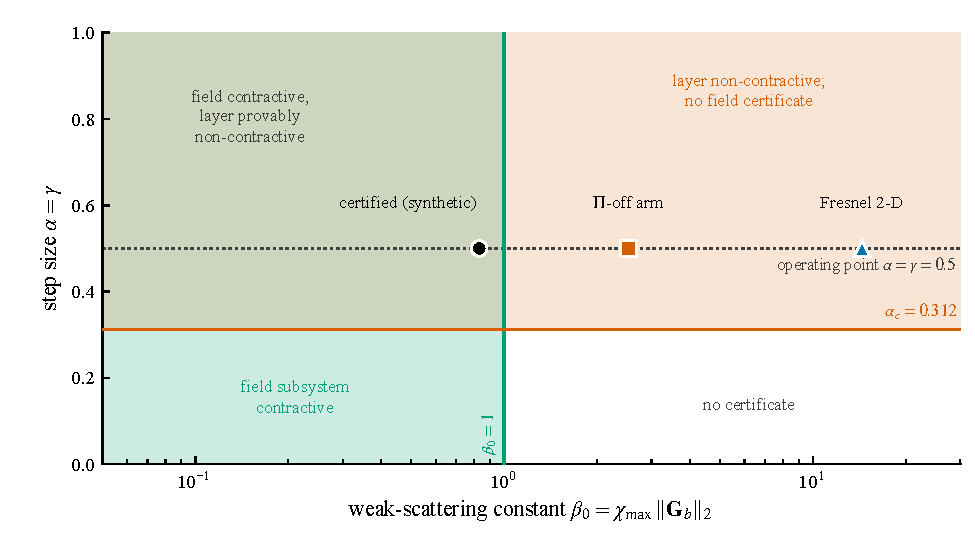
\includegraphics[width=\linewidth]{figures/fig_regime.pdf}
\caption{Regimes in the $(\beta_0,\alpha)$ plane. Left of $\beta_0=1$ the field subsystem is
provably contractive, above $\alpha=\alpha_c$ the composite layer is provably non-
contractive, and their overlap is the certified configuration. The three markers are the
synthetic box, the arm retrained without the projection, and the Fresnel geometry.}
\label{fig:regime}
\end{figure}

\begin{Theorem}[A-priori field-subsystem contraction]\label{thm:field}
Fix any admissible contrast with $\infn{\chi}\le\chi_{\max}$. Then for every $\alpha\in(0,1]$
the damped field step \eqref{eq:fieldstep} is affine in $w$ with Jacobian
$J_w=(1-\alpha)I+\alpha\,\mathrm{diag}(\chi)\mathbf{G}_b$, and
\begin{equation}\label{eq:fieldcontract}
\norm{J_w}_2 \;\le\; 1-\alpha\,(1-\beta_0),\qquad
\beta_0=\chi_{\max}\norm{\mathbf{G}_b}_2 .
\end{equation}
In particular, if $\beta_0<1$ the field subsystem is a contraction in the contrast source for
\emph{every} step size, with rate $1-\alpha(1-\beta_0)$.
\end{Theorem}
\begin{proof}
$\norm{\mathrm{diag}(\chi)\mathbf{G}_b}_2\le\infn{\chi}\norm{\mathbf{G}_b}_2\le\beta_0$, hence
$\norm{J_w}_2\le(1-\alpha)+\alpha\beta_0$.
\end{proof}
In our discretization $\norm{\mathbf{G}_b}_2=\numv{\gbnorm}$ and $\chi_{\max}=\numv{\chimax}$ give
$\beta_0=\numv{\betacert}<1$: the weak-scattering regime is \emph{certifiable before any training},
and it is the only ingredient of the theory that is a property of the physics rather than of the
learned parameters.

\begin{Theorem}[Certified boundedness of the rollout]\label{thm:bounded}
Assume (i) the physics-prior projection $\chi\leftarrow\Pi_{[0,\chi_{\max}]}(\chi)$ is applied after
every layer; (ii) $\beta_0<1$; and (iii) the initial contrast satisfies
$\infn{\chi^{0}}\le\chi_{\max}$, and $\inf_k\theta_k\alpha_k>0$ so that the per-layer rates $1-\theta_k\alpha_k(1-\beta_0)$ admit a uniform upper bound strictly below $1$. Then for every $K\ge0$, every trained parameter set and every
damping/relaxation sequence $\{(\alpha_k,\gamma_k,\theta_k)\}\subset(0,1]^{3}$,
\begin{equation}\label{eq:box}
\begin{aligned}
&\infn{\chi^{K}}\le\chi_{\max},\qquad
\norm{w^{K}}\le(\gamma_w^{+})^{K}\norm{w^{0}}
+\frac{\bar\theta\bar\alpha\,\chi_{\max}\norm{E^i}}{1-\gamma_w^{+}},\\
&\gamma_w^{+}=1-\underline{\theta\alpha}\,(1-\beta_0),\qquad
\underline{\theta\alpha}:=\inf_k\theta_k\alpha_k>0,\qquad
\bar\theta\bar\alpha:=\sup_k\theta_k\alpha_k\le1,
\end{aligned}
\end{equation}
where $\gamma_w^{+}$ is the \emph{largest} per-layer rate,
$\gamma_w^{+}=\sup_k\big(1-\theta_k\alpha_k(1-\beta_0)\big)$; because $\gamma_w^{+}\ge1-\theta_k\alpha_k(1-\beta_0)$ for every
$k$, the recursion is bounded above by a geometric sum with ratio $\gamma_w^{+}<1$. The trajectory
therefore never leaves the explicit compact set
$B=\{\infn{\chi}\le\chi_{\max}\}\times\{\norm{w}\le
\max\big(\norm{w^{0}},\;\chi_{\max}\norm{E^i}/(1-\gamma_w^{+})\big)\}$,
independently of depth; if $\norm{w^{0}}\le\chi_{\max}\norm{E^i}/(1-\gamma_w^{+})$ the box is
$B=\{\infn{\chi}\le\chi_{\max},\ \norm{w}\le\chi_{\max}\norm{E^i}/(1-\gamma_w^{+})\}$ and the
$(\gamma_w^{+})^{K}$ term is unnecessary.
\end{Theorem}
\begin{proof}
The $\chi$-bound is the definition of $\Pi$. For the field variable, taking the norm of
$w^{k+1}=w^{k}+\theta_k\alpha_k\big(\chi^{k}\odot(E^i+\mathbf{G}_b w^{k})-w^{k}\big)$ and using
$\norm{\mathrm{diag}(\chi)\mathbf{G}_b}_2\le\beta_0$ gives
$\norm{w^{k+1}}\le\big[1-\theta_k\alpha_k(1-\beta_0)\big]\norm{w^{k}}
+\theta_k\alpha_k\chi_{\max}\norm{E^i}$, an affine recursion whose per-layer rate
$1-\theta_k\alpha_k(1-\beta_0)$ is bounded above by its supremum
$\gamma_w^{+}=1-\underline{\theta\alpha}(1-\beta_0)$ (with $\underline{\theta\alpha}=\inf_k\theta_k\alpha_k>0$),
and whose forcing is bounded above by $\bar\theta\bar\alpha\chi_{\max}\norm{E^i}$; iterating gives
\eqref{eq:box}, and the transient term is needed only when $\norm{w^0}$ starts outside the stationary
radius.
\end{proof}
The three hypotheses are discharged at the operating point, not assumed. (i) is a structural flag
that every certified arm sets; (ii) is the certified $\beta_0=\numv{\betacert}$; and (iii) holds by
construction of the parameterisation, because the step sizes are
$\alpha_k=a_{\max}\sigma(a_k)$, $\gamma_k=g_{\max}\sigma(g_k)$ with $\sigma$ the logistic function
and $\theta_k\equiv1$, so each lies in $(0,a_{\max}]$ for every layer and every training iterate and
the infimum over the finitely many layers is a strictly positive minimum. What is not structural is
the \emph{value} of that minimum: it is learned, so training sets the width of the box, not its
existence.
Two points deserve emphasis. First, hypothesis (i) is the
\emph{only} place where the bound on $\chi$ enters; a network trained without $\Pi$ may still happen
to stay bounded, but the corresponding bound must then be \emph{measured}, and in our experiment the
measured value $\infn{\chi}=\numv{\NumMeasChiNoProj}$ gives
$\beta_0^{\mathrm{meas}}=\numv{\NumBetaMeas}>1$, so the theorem's hypothesis fails and no a-priori
statement survives. Second, the correction $H_k$ does not enter the box at all: it is applied to the contrast channel
ahead of $\Pi$, which clamps the result to $[0,\chi_{\max}]$ for \emph{any} correction, and the field
recursion contains no $H_k$. The role of a bounded correction lies elsewhere: the fidelity radius
$\bar\epsilon/(1-\rho_\chi)$ of Corollary~\ref{cor:fidelity} is finite only when the drift
$\norm{\hat G-F}_\infty$ is, which is supplied by the amplitude budget and, more fundamentally, by
bounding the trunk input, together with Remark~\ref{rem:featscale}.

\begin{Corollary}[Conditional drift bound for infinite-depth extrapolation]\label{cor:fidelity}
Define the \emph{physical contrast map} and its fixed point by
\begin{equation}\label{eq:chistar}
F(\chi):=\Pi\big(\hat\chi^{\mathrm{LS}}\big(E(\chi);y\big)\big),\qquad
\chi^{\star}:=F(\chi^{\star}),
\end{equation}
where $E(\chi)=E^i+\mathbf{G}_b w(\chi)$ and $w(\chi)$ solves the discrete field equation
$w=\chi\odot(E^i+\mathbf{G}_b w)$ for the given $\chi$; thus $\chi^{\star}$ is precisely the
$\chi$-component of the physical fixed point $z^{\star}$ of Proposition~\ref{prop:fixpoint}. For the
cyclic composite $T^{P}:=T\circ\cdots\circ T$ of $P$ copies of the repeated trained layer, define
the \emph{corrected contrast map} by $\hat G(\chi):=\pi_\chi\big(T^{P}(\chi,w(\chi))\big)$, using
the \emph{same exact field solution} $w(\chi)$ as $F$; $\hat G$ is therefore a \emph{proxy}: it resets
the field to the exact solution after every period, whereas the true rollout keeps the damped field
update, so $\hat G$'s fixed point need not coincide with the fixed point of the repeated layer $T^P$,
and (c) below bounds the distance to $\chi^\star$ only for this proxy. Assume
(a) $\hat G$ has a fixed point $\hat\chi\in B$; (b) $F$ is globally Lipschitz on $B$ with
constant $\rho_\chi<1$, i.e.\ $\sup_{\chi\in B}\norm{DF(\chi)}_2<1$, which is strictly stronger
than a pointwise spectral radius condition; and (c) $\sup_{\chi\in B}\norm{\hat G(\chi)-F(\chi)}\le\delta_{\mathrm{GF}}$, where
$\delta_{\mathrm{GF}}$ is the \emph{drift} of the corrected map from the physical map and is a
\emph{separate} constant from the trunk amplitude budget $\bar\epsilon$ of \eqref{eq:budgets}: the two
are not equal in general. With $H\equiv0$ the drift is not zero but the relaxation bias between one
exact contrast update and $P$ damped layers, and it is not controlled by $\bar\epsilon$ either.
Then
\begin{equation}\label{eq:fidelity}
\norm{\hat\chi-\chi^{\star}}\;\le\;\frac{\delta_{\mathrm{GF}}}{1-\rho_\chi}.
\end{equation}
If in addition (d) $\hat G$ is $\hat\rho$-Lipschitz on $B$ with $\hat\rho<1$, then $\hat\chi$ is the
unique fixed point of $\hat G$ in $B$ and iterating $\hat G$ reaches accuracy $\delta$ in
$O\big(\log(1/\delta)/\log(1/\hat\rho)\big)$ layers.
\end{Corollary}
\begin{proof}
$\norm{\hat\chi-\chi^{\star}}=\norm{\hat G(\hat\chi)-F(\chi^{\star})}
\le\norm{\hat G(\hat\chi)-F(\hat\chi)}+\norm{F(\hat\chi)-F(\chi^{\star})}
\le\delta_{\mathrm{GF}}+\rho_\chi\norm{\hat\chi-\chi^{\star}}$, and solving for the norm gives
\eqref{eq:fidelity}; only (b) and (c) evaluated at $\hat\chi$ are used, so this part needs no
contraction of $\hat G$. Uniqueness and the geometric rate are the Banach fixed-point theorem
applied to $\hat G$ under (d). Hypothesis (c) alone does \emph{not} make $\hat G$ a contraction: it
constrains the distance $\norm{\hat G-F}_\infty$ and says nothing about the Lipschitz constant of
$\hat G$, and a bounded-distance perturbation of a contraction may have an arbitrarily large
Lipschitz constant, a bump of height $\bar\epsilon$ and arbitrarily small width satisfies (c)
while its Lipschitz constant grows without bound. Uniqueness and the $O(\log(1/\delta))$ rate
therefore rest on the separate hypothesis (d), which we do not claim to hold here; in our
measurements even the weaker (b) fails.
\end{proof}
The hypothesis is placed on $F$, the map that \emph{defines} $\chi^{\star}$, not on the corrected
map $\hat G$; the two agree only where $H\equiv0$. Two caveats follow, and are \emph{not}
hypotheses we can discharge here.

First, $\rho_\chi<1$ is an assumption, not a theorem: the only contraction constant available
a~priori is $\beta_0<1$, which bounds the \emph{field} subsystem \eqref{eq:fieldcontract} and says
nothing about $F$. Indeed
$\partial F/\partial\chi=(\partial\hat\chi^{\mathrm{LS}}/\partial E)(\partial E/\partial\chi)$ with
$\norm{\partial E/\partial\chi}_2\le\norm{\mathbf{G}_b}_2/(1-\beta_0)=\numv{\NumdEdChi}$, while
$\partial\hat\chi^{\mathrm{LS}}/\partial E$ is amplified by the inverse of the (regularized) normal
matrix, whose smallest eigenvalue is $\numv{\NumLamMin}$; substituting $\beta_0$ for $\rho_\chi$ in
the radius is therefore unjustified, and $\bar\epsilon/(1-\beta_0)$ must not be quoted as an
``a-priori drift radius''. For both $F$ and $\hat G$ we report two numbers, the $\sigma_{\max}$ of
the $\chi\!\to\!\chi$ block and the norm of the whole $\chi$-row $[A\,B]$, the latter being the
Lipschitz constant of the $\chi$-map and the former only a lower bound on it, as reported in the
experimental section. These numbers do \emph{not} all fall on one side of one: in the constrained arm
every pair is below one (on $\hat G$, $\numv{\NumRhoChiCons}$ and $\numv{\NumChiLipRowCons}$; on $F$,
$\numv{\NumChiFBlockCons}$ and $\numv{\NumChiLipRowFCons}$), so nothing measured there refutes
$\rho_\chi<1$, whereas in the unconstrained arm the row norm of $\hat G$ reaches
$\numv{\NumChiLipRowUnc}$ and does refute it. Neither arm is \emph{verified} either: the block value is
a lower bound and the row norm is exact only for the layer map, while the reduced $\chi$-map derivative
is a Schur complement whose norm neither of them bounds. We therefore report the measurement arm by
arm and do not claim a general failure of the geometric hypothesis. The certified content of the theory is therefore
the boundedness of Thm.~\ref{thm:bounded} plus the field-subsystem rate of
Thm.~\ref{thm:field};
Corollary~\ref{cor:fidelity} supplies \emph{no} finite a-priori radius, and reporting the measured
$\rho_\chi$ in its place is the accounting we use.

Second, the conditional character of Corollary~\ref{cor:fidelity} is a direct price of modelling
multiple scattering. In the single-scattering Born linearization the field used by the contrast
step is the fixed $E^i$, so $\partial\hat\chi^{\mathrm{LS}}/\partial\chi=0$, $F$ is a constant map,
$\rho_\chi=0$, and \eqref{eq:fidelity} becomes the unconditional radius $\bar\epsilon$. It is
precisely the self-consistency of $E$ with $\chi$, the feature that makes the method work for
strong scatterers, that makes the radius conditional.

\begin{Proposition}[Exact finite-depth noise accounting]\label{prop:noise}
Let $L_k:=\operatorname{Lip}\big(T_k(\cdot;y)\big)$ and
$\Lambda_k:=\sup_{z\in B}\norm{T_k(z;y+\Delta y)-T_k(z;y)}/\norm{\Delta y}$. Then for every
$K\ge1$ and every bounded $\Delta y$,
\begin{equation}\label{eq:noiseexact}
\norm{z^{K}(y+\Delta y)-z^{K}(y)}
\;\le\;\Big[\sum_{k=0}^{K-1}\Lambda_k\!\!\prod_{j=k+1}^{K-1}\!\!L_j\Big]\norm{\Delta y}.
\end{equation}
\end{Proposition}
\begin{proof}
Let $z^{k},\tilde z^{k}$ be the clean and perturbed trajectories. Since $T_k(\cdot;y)$ and
$T_k(\cdot;y+\Delta y)$ share a base point,
$\norm{\tilde z^{k+1}-z^{k+1}}
\le L_k\norm{\tilde z^{k}-z^{k}}+\Lambda_k\norm{\Delta y}$. Iterating the affine recursion from
$\tilde z^{0}=z^{0}$ and collecting the geometric products gives \eqref{eq:noiseexact}.
\end{proof}
Equation~\eqref{eq:noiseexact} is exact and makes no contraction assumption. With a cyclic schedule
of period $P$ the per-period amplification is $\Pi_{j=1}^{P}L_j$, so the noise gain is bounded
uniformly in depth when $\Pi_{j=1}^{P}L_j<1$; at the equality $\Pi_{j=1}^{P}L_j=1$ the per-cycle
injection $\sum_{j=1}^{P}\Lambda_j$ accumulates linearly with the number of cycles, so equality is
not sufficient for a uniform bound without an additional decay assumption. This is the sharp
statement; the familiar closed form is a special case, and we state it as such. Neighbouring work studies stability of unfolded forward-backward to data perturbations \cite{devalle2023}; our bound is for the contrast-source composite, is exact rather than perturbative, and needs no contraction assumption.

\begin{Corollary}[Geometric bound]\label{cor:noisegeo}
If in addition $L_j\le\rho<1$ for all $j$, then
\eqref{eq:noiseexact} $\le\Lambda(1-\rho^{K})/(1-\rho)\norm{\Delta y}
\le\Lambda\norm{\Delta y}/(1-\rho)$.
\end{Corollary}
\begin{proof}
Each product in \eqref{eq:noiseexact} is at most $\rho^{K-k}$; the geometric sum follows.
\end{proof}
This bound is \emph{conditional}, and in our setting its hypothesis fails by our own measurement:
$L_j=\sigma_{\max}(J_j)$ is exactly the quantity that Proposition~\ref{prop:imposs} proves to exceed
one for $\alpha>\alpha_c$, with measured values
$\sigma_{\max}(J)=\numv{\NumPhysSigma}$ at $\alpha=\gamma=\tfrac12$ and
$L\in[\numv{\NumSigMin},\numv{\NumSigMax}]$ over the converged fixed-step grid of
$\numv{\NumAlphaSweepN}$ discrete step sizes spanning $\alpha=\gamma\in[0.05,1]$, \emph{every}
point of which is non-contractive, not only those
above $\alpha_c$ as measured in the experimental section; at the learned step sizes the $K{=}8$ cyclic composite
is $\numv{\NumSigCompCons}$. We therefore do not present $\Lambda/(1-\rho)$ as a result about this
architecture; it is stated only to expose the hypothesis, which is contradicted by the same
experiments that would otherwise be cited in its support. The operative statement is
Proposition~\ref{prop:noise}.

\begin{Corollary}[Spectral-radius form for non-normal layers]\label{cor:noisenormal}
Assume the layer Jacobian is uniformly bounded on $B$: for every $z\in B$ and every $m\le K$,
$\norm{DT(z)^{m}}\le\kappa\rho^{m}$, with $\rho=\sup_{z\in B}\rho(DT(z))<1$ and
$\kappa=\sup_{z\in B}\kappa_2(V(z))$. Then in particular $\norm{DT(z)}\le\kappa\rho$ for all
$z\in B$, so the Jacobian of the composite $T_{K-1}\circ\cdots\circ T_{k+1}$ , a product of state-dependent Jacobians along the trajectory, is bounded by $(\kappa\rho)^{K-1-k}$, and
\eqref{eq:noiseexact} is at most
$\Lambda\norm{\Delta y}\,(1-(\kappa\rho)^{K})/(1-\kappa\rho)$ whenever $\kappa\rho<1$.
\end{Corollary}
\begin{proof}
By the chain rule the composite Jacobian is $DT(z_{K-1})\cdots DT(z_{k+1})$, a product of
\emph{different} state-dependent matrices, not a single matrix power; the identity $\norm{J_{K-1}\cdots J_{k+1}}=\norm{J^{K-1-k}}$ holds only at the fixed point, where all factors coincide. The
hypothesis with $m=1$ gives $\norm{DT(z)}\le\kappa\rho$ for every $z\in B$, hence the product is
bounded by $(\kappa\rho)^{K-1-k}$ for every trajectory in $B$; summing the $K$ terms of
\eqref{eq:noiseexact} yields the stated factor. Because $\kappa=\sup_{z\in B}\kappa_2(V(z))$ is not bounded by the present measurements, only the lower bound $M_J$ of Remark~\ref{rem:mj} being available, and because $\rho<1$ alone does not control the product of non-normal factors, the corollary does
\emph{not} yield a finite noise gain from the current data; it is stated only to expose the hypothesis.
\end{proof}
\begin{Remark}[Transient factor]\label{rem:mj}
The transient $M_J:=\sup_{1\le m\le K}\norm{J^{m}}$ is the amplification a practitioner is tempted
to substitute for the Lipschitz constant, and we measure it below; the substitution is nevertheless
\emph{invalid}. From $\rho^{m}\le\norm{J^{m}}\le\kappa_2(V)\rho^{m}$ we get $M_J\le\kappa_2(V)$, so
$M_J$ is a \emph{lower} bound on the factor the geometric sum requires, while
$(1-\rho^{K})/(1-\rho)$ attaches to $\kappa_2(V)$ and not to $M_J$. Multiplying the two, which is
what a bound of the form $\Lambda\norm{\Delta y}M_J(1-\rho^{K})/(1-\rho)$ would do, can
\emph{understate} the true amplification, and no such product bound exists in general. It fails
already for the normal $J=0.5I$ with $K=3$, where the exact factor
$\sum_{k=0}^{K-1}\prod_{j=k+1}^{K-1}L_j$ of \eqref{eq:noiseexact} is $1.75$ while
$M_J(1-\rho^{K})/(1-\rho)=0.875$; and it fails outright when $J$ is not diagonalisable, e.g.\ the
nilpotent $J=\bigl[\begin{smallmatrix}0&10\\0&0\end{smallmatrix}\bigr]$ with $K=3$, where the exact
factor is $10^2+10+1=111$ ($\sigma_{\max}(J)=10$), while $\rho=0$ and $\kappa_2(V)=\infty$. The crudest bound available from $M_J$ is the
term-counting $\sum_{m\le K}\norm{J^{m}}\le K M_J$; it is not the only one (e.g.\
$\sum_{k<K}\Lambda_k\norm{J^{K-1-k}}\le\Lambda_{K-1}+M_J\sum_{k<K-1}\Lambda_k$ also uses $M_J$
alone), and we claim nothing stronger than that every such bound is crude in the same way. In short, $M_J$ and
$\kappa_2(V)$ coincide only for normal operators, precisely the case in which the spectral radius
\emph{is} a Lipschitz constant. We report $M_J$ because it is recomputable and because its ratio to
$\rho$ measures the non-normality, not because it bounds the noise gain.
\end{Remark}
Corollaries~\ref{cor:noisegeo} and~\ref{cor:noisenormal} differ by exactly the factor $\kappa_2(V)$:
replacing the Lipschitz constant by the spectral radius is only legitimate for normal
operators, and the layer map here is emphatically non-normal. The cost of that replacement is
measurable, and we measure its ingredients: for the $K{=}8$ cyclic composite
$M_J=\numv{\NumMJCons}$, a lower bound on $\kappa_2(V)$ (Remark~\ref{rem:mj}), against
$\rho=\numv{\NumRhoComp}$ and $\sigma_{\max}=\numv{\NumSigCompCons}$, giving a non-normality gap
$\sigma_{\max}/\rho=\numv{\NumGapRatio}$ as reported in the experimental section. These three belong to one and
the same operator, the composite Jacobian of the $K{=}8$ rollout, and are reported
together for that reason; the per-layer value at fixed $\alpha=\gamma=\tfrac12$,
$\numv{\NumSigCompLayerCons}$, is a different operator and is listed separately. This is the quantitative measure of
how much a spectral-radius-based bound would understate the transient. The value of $M_J$ depends on
where the horizon is truncated: over the full horizon $m\in\{1,2,4,8\}$ the same composite reaches
$\numv{\NumMJFullCons}$ at $m=\numv{\NumMJFullArgmaxM}$ (constrained) and $\numv{\NumMJFullUnc}$ at
$m=\numv{\NumMJFullArgmaxMUnc}$ (unconstrained), so the depth-2 truncation is not a benign
simplification and we report both.

\begin{table}[htbp]
\centering
\caption{What each noise-analysis quantity is for, and what this paper establishes about it.
Only the first row is a usable ingredient of a bound; the second is a diagnostic; the last three
are hypotheses the paper does not establish, one of them refuted by measurement.}
\label{tab:noisestatus}
\small
\begin{tabular}{@{}p{0.10\linewidth}p{0.36\linewidth}p{0.44\linewidth}@{}}
\toprule
quantity & role & status in this paper \\
\midrule
$\Lambda$ & sensitivity of one layer to a data perturbation & bounded explicitly by
\eqref{eq:Lambda} from the Tikhonov floor and the amplitude budget, and measured
($\numv{\NumLambdaMeas}$ against $\numv{\NumLambdaBound}$) \\
$M_J$ & transient amplification $\sup_{m\le K}\norm{J^{m}}$ over the horizon & computable
($\numv{\NumMJCons}$ at $K{=}8$); a \emph{lower} bound on $\kappa_2(V)$, not a substitute for it \\
$\kappa_2(V)$ & non-normality factor of the geometric form & no uniform upper bound available;
the corollary that needs it therefore yields no finite gain \\
$\rho<1$ & hypothesis of the geometric bound & refuted by measurement: $\sigma_{\max}>1$ at every
point of the step-size grid \\
$\rho_\chi<1$ & hypothesis of the fidelity radius $\delta_{\mathrm{GF}}/(1-\rho_\chi)$ & neither
verified nor refuted: the block value is below one ($\numv{\NumRhoChiCons}$) but it is only a lower
bound on the Lipschitz constant, whose row-norm estimate is $\numv{\NumChiLipRowCons}$ \\
\bottomrule
\end{tabular}
\end{table}
Table~\ref{tab:noisestatus} is the honest summary of where the noise analysis stands: it supplies a
\emph{conditional} error-accounting framework and an exactly computable depth-$K$ factor, not a
certified noise gain, and nothing below presents it as one.

Finally, $\Lambda$ itself can be bounded explicitly rather than asserted. A layer depends on the
data through two channels: the regularized least-squares contrast step
$\hat\chi^{\mathrm{LS}}=A(E)^{-1}b(E,y)$, for which
$\partial b/\partial y=\mathrm{diag}(\bar E)\mathbf{G}_s^{H}$ and hence
$\norm{\partial\hat\chi^{\mathrm{LS}}/\partial y}_2
\le\max_r|E(r)|\,\norm{\mathbf{G}_s}_2/\lambda_{\min}(A)$ here the $\ell_\infty$ field norm is the
correct one, because $b$ is linear in $y$ with coefficient $\mathrm{diag}(\bar E)$; and the learned
correction, which sees $y$
through the adjoint residual $\mathbf{G}_s^{H}(\mathbf{G}_s w^{+}-y)$ with
$\norm{\partial(\cdot)/\partial y}_2=\norm{\mathbf{G}_s}_2$, attenuated by the feature scale of the
residual channel and the spectral clamp. Combining,
\begin{equation}\label{eq:Lambda}
\Lambda\;\le\;\norm{\mathbf{G}_s}_2
\Big[\frac{\theta\gamma\max_r|E|}{\lambda_{\min}(A)}
\;+\;\frac{\bar\epsilon}{s_{\mathrm{res}}}\prod_i\norm{W_i}_2\Big],
\end{equation}
i.e.\ the sensitivity of the $\chi$-step is controlled by the Tikhonov floor
$\lambda_{\min}(A)\ge c_{\mathrm{cg}}\min_j\sum_i|E_{ij}|^{2}\norm{\mathbf{G}_s(\cdot,j)}_2^{2}$ that
the implementation adds, and the correction channel by the amplitude budget. Measured directly,
$\Lambda=\numv{\NumLambdaMeas}$ against the contrast-channel bound $\numv{\NumLambdaBound}$ with
$\lambda_{\min}(A)=\numv{\NumLamMin}$ and $s_{\mathrm{res}}=\numv{\NumScaleRes}$
in the experimental section; the correction term is negligible at the trained weights. Equation
\eqref{eq:Lambda} replaces an earlier assertion of ours that $\Lambda$ is bounded ``by construction'':
the construction is \eqref{eq:Lambda}, and it is only as good as the Tikhonov floor, so
$\lambda_{\mathrm{rel}}$ must not be driven to zero.

\begin{Proposition}[Depth--accuracy--stability trade-off]\label{prop:tri}
Fix a correction architecture and let $\mathcal{H}(\bar\epsilon,\ell)$ be the class of admissible
corrections, assumed nested: $\bar\epsilon_1\le\bar\epsilon_2$ and $\ell_1\le\ell_2$ imply
$\mathcal{H}(\bar\epsilon_1,\ell_1)\subseteq\mathcal{H}(\bar\epsilon_2,\ell_2)$. Then
(i) \emph{[depth]} under hypotheses (a)--(d) of Corollary~\ref{cor:fidelity}, the $K$-step iterate
of $\hat G$ satisfies $\norm{\hat G^{K}(\chi^{0})-\chi^{\star}}\le\hat\rho^{K}\norm{\chi^{0}-\chi^{\star}}
+\delta_{\mathrm{GF}}(1+\hat\rho^{K})/(1-\rho_\chi)$: a geometrically decaying depth term plus a floor that
does not vanish with $K$ (the decay uses (d), $\hat G$'s own modulus; hypothesis (c) alone gives no
decay);
(ii) \emph{[magnitude budget, proved]} the radius $\delta_{\mathrm{GF}}/(1-\rho_\chi)$ is strictly
increasing in $\delta_{\mathrm{GF}}$, so a larger corrected-map drift worsens the only a-priori
fidelity constant the framework provides. The relation of this drift to the trunk amplitude budget
$\bar\epsilon$ is \emph{not} asserted; the two were conflated in an earlier draft and are kept distinct
here, so certifiability and representational power pull in opposite directions through the drift budget;
(iii) \emph{[slope budget, proved]} by nestedness, tightening $\ell$ shrinks $\mathcal{H}$, hence
cannot lower the best attainable data misfit over the class, and cannot raise the certified radius
either, since the radius depends on the drift $\delta_{\mathrm{GF}}$ alone and not on the trunk amplitude budget $\bar\epsilon$, whose relation to the drift is not established here.
The two budgets therefore act through disjoint knobs, magnitude controls the certificate, slope
controls which corrections are representable, and there is no single ``tightening'' that improves
both. Empirically, as shown in the experimental section, over
$\bar\epsilon\in[\numv{\NumEbWorst},\numv{\NumEbBest}]$ both the reconstruction error and the
noise sensitivity improve as $\bar\epsilon$ grows, i.e.\ the magnitude budget is \emph{not} the
binding constraint in this regime; the binding trade-off is the one between the budgeted and the
unbudgeted families.
\end{Proposition}
\begin{proof}
(i) follows from the contraction inequality
$\norm{\hat G^{K}(\chi^{0})-\hat\chi}\le\hat\rho^{K}\norm{\chi^{0}-\hat\chi}$ of hypothesis (d)
combined with Corollary~\ref{cor:fidelity}:
$\norm{\hat G^{K}(\chi^{0})-\chi^{\star}}\le\hat\rho^{K}\norm{\chi^{0}-\chi^{\star}}
+\hat\rho^{K}\delta_{\mathrm{GF}}/(1-\rho_\chi)+\delta_{\mathrm{GF}}/(1-\rho_\chi)$. (ii) is immediate from
$\partial_{\bar\epsilon}\big[\bar\epsilon/(1-\rho_\chi)\big]=1/(1-\rho_\chi)>0$. (iii): nestedness
gives $\min_{H\in\mathcal{H}(\bar\epsilon,\ell_1)}(\text{misfit})\ge
\min_{H\in\mathcal{H}(\bar\epsilon,\ell_2)}(\text{misfit})$ for $\ell_1\le\ell_2$ , since a minimum over a smaller set is not smaller,, and the radius is a function of $\bar\epsilon$ alone.
\end{proof}

\begin{Remark}[Averaged layers as a restriction]\label{rem:averaged}
$\beta_0<1$ restricts the a-priori field certificate to weak-to-moderate contrasts. One may
\emph{impose} nonexpansiveness by replacing each layer with an averaged form
$T_k=(1-\omega_k)I+\omega_kM_k$ with $M_k$ nonexpansive and $\omega_k\in(0,1)$, so
$\omega_k$ is a different object from the code-level relaxation $\theta_k$ of \eqref{eq:layer-code};
the two are distinguished by their symbols and their scope. Compositions of averaged operators are
averaged, so the infinite-depth limit exists. This is a \emph{design restriction}, not a rewriting of
the faithful composite: Proposition~\ref{prop:imposs} shows that on $\alpha>\alpha_c$ the faithful
layer cannot be put in this form with $\sigma_{\max}\le1$, and the averaged construction obtains its
guarantee by reducing the effective correction strength $\omega_k$, which is exactly the accuracy
price quantified in Proposition~\ref{prop:tri}. It is therefore an option with an explicit cost, not a route
around Proposition~\ref{prop:imposs}, which is the statement about the architecture as trained.
\end{Remark}

\begin{Remark}[Scope of the feature scales]\label{rem:featscale}
In the implementation the state-to-feature map is $f\mapsto\tanh(f/s_c)$, channel-wise, with the
hand-set scales $s_c$ of Sec.~\ref{sec:training}. The scales dominate the per-channel Lipschitz
bounds. The residual channel obeys
$\operatorname{Lip}\le\norm{\mathbf{G}_s}_2^{2}=\numv{\NumLipResidChan}\ll s_{\mathrm{res}}=2$;
the field channel obeys $\operatorname{Lip}\le\norm{\mathbf{G}_b}_2=\numv{\gbnorm}<s_E=3$; and the
state channels obey $\operatorname{Lip}\le1<s=2$. Every channel is
normalised to Lipschitz constant at most one \emph{individually}. The joint state-to-feature map is \emph{not} $1$-Lipschitz: stacking the channels gives the bound
$\big(\sum_c(\operatorname{Lip}_c/s_c)^{2}\big)^{1/2}=\numv{\NumFeatJointLip}$, which exceeds one.
The saturation guarantees boundedness of the \emph{range}: every feature entry lies in
$[-1,1]$, so the trunk input is bounded uniformly over the state, which is what makes the
amplitude budget $\bar\epsilon$ attainable by construction and what prevents the correction from
growing with the state. The nominal slope budget is not the realised one: the operators certified at inference time are
the \emph{measured} $\ell=\operatorname{Lip}(H_k)$ and
$\bar\epsilon$, reported in the experimental section.
\end{Remark}

\begin{Remark}[Relation to LISTA coupling]
LISTA-CP \cite{listacp} constrains the two learnable matrices of each layer by the
\emph{equality} $W_1^kA+W_2^k=I$, coupling them to the known measurement matrix $A$. The connection to our construction is a family resemblance rather than an analogy: both tie the learnable part to a known operator, but LISTA-CP does so by an equality
constraint on weights while we impose a Lipschitz (amplitude) budget and a per-kernel spectral
clamp, a neighbourhood condition, not an equality, and the guaranteed object is not the
recovery of a sparse code, which we do not address, but the fixed point and the boundedness of the
physical iteration.
\end{Remark}

The statements of this section are not independent, and the two kinds of relation between them
should be kept apart.
Prop.~\ref{prop:tri} is a \emph{consequence} of the results above: it combines the per-layer
non-contractivity of Prop.~\ref{prop:imposs} with the field-subsystem rate of
Thm.~\ref{thm:field} and the confinement of Thm.~\ref{thm:bounded}, and it would not survive the
removal of any one of the three. Remarks~\ref{rem:averaged} and~\ref{rem:featscale}, and the
closing remark on LISTA coupling, are \emph{independent} observations of a different kind: they record what must be given up, such as an averaged operator, tighter feature scales or a LISTA-type equality constraint on the weights, to recover a contraction that the faithful composite does
not have, and none of them is used in the proof of Thm.~\ref{thm:field} or
Thm.~\ref{thm:bounded}.

\section{Constrained Training Scheme}\label{sec:training}
The construction below enforces the hypotheses that are \emph{within our control}: a bounded, additive, contrast-channel correction, which bounds the fidelity drift $\norm{\hat G-F}_\infty$ of Cor.~\ref{cor:fidelity} and not the invariant box of Thm.~\ref{thm:bounded}, and a physics core that is contracting in the field variable for every step
size by Thm.~\ref{thm:field}. The construction does \emph{not} control the layer Lipschitz constant
$\ell$ entering Prop.~\ref{prop:imposs}, nor the composite constant $\rho_\chi$ entering
Cor.~\ref{cor:fidelity}: those are measured after training and reported, because
Prop.~\ref{prop:imposs} already shows that the contraction hypotheses they need cannot be arranged
by construction.

\subsubsection{Amplitude--slope parameterization}
Each correction is
\begin{equation}\label{eq:param}
H_k(z;y) \;=\; \bar\epsilon\,\tanh\!\big(U_k(z;y)\big),
\end{equation}
where $U_k$ is a CNN trunk. Since $\tanh$ is $1$-Lipschitz and bounded by $1$:
(a) $\norm{H_k}\le\bar\epsilon$ for every input, the amplitude budget;
(b) $\operatorname{Lip}(H_k)\le\bar\epsilon\prod_l\sigma_l(U_k)$, where $\sigma_l$ are the
spectral norms of the kernels. Clamping every output-row block of each kernel to $\sigma_l\le1$ is hard spectral normalization: after each optimizer step we rescale $W\leftarrow W/\max(1,\hat\sigma(W))$, with $\hat\sigma$ from eight power iterations. This is a \emph{sufficient} condition for the nominal slope budget
$\operatorname{Lip}(H_k)\le\bar\epsilon$; this is a design target on the per-kernel
operator norms, whereas the quantity that enters Prop.~\ref{prop:imposs} and
Cor.~\ref{cor:fidelity} is the \emph{measured} $\operatorname{Lip}(H_k)$ of the composed trunk,
which we report in the experimental section and do not assume. The two knobs are independent:
$\bar\epsilon$ fixes \emph{how much} the network may move the physical fixed point, as Cor.~\ref{cor:fidelity} bounds it; the spectral clamp controls \emph{how fast} successive layers may move
it.

\subsubsection{Feature boundedness}
The trunk input concatenates the adjoint-projected data residual, the fields, the contrast source
and the contrast. We pass it through $\tanh(\cdot/s_c)$ with fixed per-channel scales $s_c$ chosen
\emph{above} the a-priori sensitivity of each channel; the per-channel bounds and the resulting
joint constant are given in Remark~\ref{rem:featscale}. The guarantee obtained here is
\emph{boundedness of the range}, not $1$-Lipschitzness of the joint map: every feature entry lies in
$[-1,1]$ regardless of the state, so the trunk input cannot grow with the state and $\norm{H_k}$ is
finite by construction, which keeps the drift $\norm{\hat G-F}_\infty$ of
Cor.~\ref{cor:fidelity} under the amplitude budget and makes the slope budget \eqref{eq:param}
non-vacuous ($\tanh$ alone saturates only asymptotically). The third ablation arm of Sec.~\ref{sec:exp} isolates this effect.

\subsubsection{Physics-prior projection}
The contrast is constrained to the physically admissible box after every layer,
\begin{equation}\label{eq:proj}
\chi \;\leftarrow\; \Pi_{[0,\chi_{\max}]}(\chi),
\end{equation}
a nonexpansive projection onto a closed convex set that contains the true contrast of the
admissible class studied here. The non-negativity of $\chi$ is a property of that class, 
lossless dielectrics at least as dense as the background, $\varepsilon_r\ge\varepsilon_b$, and
\emph{not} a consequence of passivity alone, which would also admit $-1<\chi<0$; the calibration
data are generated with $0.25\le\chi\le\chi_{\max}$ accordingly. The projection supplies
hypothesis (i) of Theorem~\ref{thm:bounded} with a \emph{known} constant,
keeps the state in the compact set on which the constants are certified, absorbs the transient
amplification of the non-normal composite by Prop.~\ref{prop:imposs}, and leaves every fixed point
that already lies in the box unchanged. Its exact role is quantified by two ablations in
Sec.~\ref{sec:exp}: it is indispensable at inference time, and it is what upgrades empirical
boundedness to a certificate.

\subsubsection{Loss and graceful degradation}
Training minimizes
$\mathcal{L}=\norm{\chi^{K}-\chi_{\mathrm{gt}}}^2+\lambda\norm{\mathbf{G}_sw^{K}-y}^2$
on synthetic pairs. Since $H_k\equiv0$ recovers the classical iteration exactly
($\bar\epsilon=0$), the constrained family searched by the optimizer is a
$\bar\epsilon$-neighborhood of the physical iteration, the learned network is a
\emph{certified perturbation} of a convergent physical scheme, never a replacement of it.

\section{Numerical Experiments}\label{sec:exp}
The classical references are the damped alternating fixed-point iteration, contrast-source
inversion (CSI)~\cite{csi_lit} and the subspace-based optimization method (SOM)~\cite{som_lit}.
The comparison below counts iterations rather than wall-clock time, and
Sec.~\ref{sec:lim}~(ix) records that CSI and SOM also remain above the unrolled networks, so the
advantage is calibrated against all three baselines rather than only the damped iteration.
\subsection{Setup}
\label{sec:setup}
We consider a 2-D TM scenario: $32\times32$ cells of side $0.02\lambda$ (DoI $0.64\lambda$),
$n_{\mathrm{inc}}=8$ plane waves ($45^\circ$ spacing), $32$ receivers on a circle of radius
$2\lambda$; MoM self-terms use the Richmond approximation. The contrast consists of $1$--$3$
ellipses/rings with $\chi\in[0.25,0.5]$; the exact discrete solution is obtained by a dense
solve of \eqref{eq:discrete} per sample. Training uses $300$ samples, Adam
($\mathrm{lr}=10^{-3}$), batch $16$, and the loss above with $\lambda=0.5$; the evaluation set is
$100$ unseen samples. The two sets are independent draws: training uses generator seed $1$ and
evaluation seed $2$, each sample drawing its own number of scatterers ($1$--$3$), their centres,
semi-axes and orientations before the forward solve, and no test object is used for training or
augmentation. There is no separate validation split, so every test number reported below is on
seed-$2$ draws that never entered training; the seed replicates reported with the extrapolation
study change the training seed as well ($11$--$14$), and their spread is what we report instead of
a cross-validation curve. The correction CNN has
two $3\times3$ convolutional layers ($8$ channels) with ReLU and a $3\times3$ output layer;
$\bar\epsilon=\numv{\epsbar}$ unless stated. The certified constants are
$\norm{\mathbf{G}_b}_2=\numv{\gbnorm}$, $\chi_{\max}=\numv{\chimax}$ and
$\beta_0=\numv{\betacert}$.
\emph{Hardware and software.} Every number reported in this paper was produced on one
workstation: an AMD Ryzen 9 5950X (16 cores, 32 threads), 32\,GB of memory and an NVIDIA
GeForce RTX 3080 Ti (12\,GB), running Windows 10 (build 19045) with Python 3.11.15,
PyTorch 2.13.0 (CUDA 12.6), NumPy 2.4.6 and SciPy 1.17.1. Training runs on the GPU in single
precision (float32 parameters, complex64 fields); the audits behind Table~\ref{tab:cert} run on
the CPU in double precision (float64 parameters, complex128 fields), and they are pinned to the
CPU on purpose so that an audit never shares the GPU with a training run. The per-layer
wall-clock surcharge of Sec.~\ref{sec:depth} is a median over seven repetitions at batch $16$
with two BLAS threads on this machine, so it characterises this implementation and not the
architecture alone.
\emph{Baselines and fairness.} We compare against (a) the classical damped alternating iteration
with $H_k\equiv0$ and (b) unconstrained unrolling, identical in architecture, parameter count,
optimizer, schedule and seed but with the budgets removed. Because the unrolled networks
\emph{learn} damping factors bounded by $\alpha_{\max}=0.5$, $\gamma_{\max}=0.6$ while the
classical baseline uses the full step $\alpha=\gamma=1$, we additionally sweep
$\alpha=\gamma\in[0.1,1]$ for the classical method at $K\in\{8,24,50,100\}$ and report its
\emph{best} configuration in Table~\ref{tab:cls}; the comparison below is therefore against a
tuned classical baseline, not an arbitrary one. The sweep is a separate driver
from the depth curve, because the classical branch itself is
untuned by design; both write to the same results directory from which Table~\ref{tab:cls} and all
numerical macros in this paper are generated, so no number here is transcribed by hand.
\subsection{Discretisation robustness}
\label{sec:grid}
We recompute the certificate ingredients at $32\times32$, $64\times64$ and
$128\times128$ cells at fixed physical domain $L=\numv{\NumGridL}\lambda$. Across a
$\numv{\NumGridFactor}$-fold cell refinement, $\norm{G_b}_2$ drifts by
$\numv{\NumGridDriftGbPct}\%$, $\beta_0$ stays below one at every grid, and the receiver
operator scales as its cell-area weight predicts, as Table~\ref{tab:grid} records. The operator-level
certificates are therefore a property of the continuous operator, not a coarse-grid artefact;
the reconstruction studies that follow use $32\times32$, noted as a limitation in
Sec.~\ref{sec:lim}.

\begin{table}[htbp]
\centering
\caption{Certificate ingredients across three discretisations at fixed physical domain $L=\numv{\NumGridL}\lambda$. The hypothesis $\beta_0<1$ holds at every grid and the operator-level quantities move by less than $1\%$.}
\label{tab:grid}
\small
\begin{tabular}{rcccc}
\toprule
$N\times N$ & $\Delta x/\lambda$ & $\norm{G_b}_2$ & $\beta_0$ & $\mathcal{E}$ \\
\midrule
$32\times32$   & $0.02$  & $\numv{\NumGridGbLo}$  & $\numv{\NumGridBetaLo}$  & $\numv{\NumGridELo}$ \\
$64\times64$   & $0.01$  & $\numv{\NumGridGbMd}$  & $\numv{\NumGridBetaMd}$  & $\numv{\NumGridEMd}$ \\
$128\times128$ & $0.005$ & $\numv{\NumGridGbHi}$ & $\numv{\NumGridBetaHi}$ & $\numv{\NumGridEHi}$ \\
\bottomrule
\end{tabular}
\end{table}

\subsection{Certificate boundary on measured data}
\label{sec:fresnel}
This subsection maps the quantitative boundary of the weak-scattering hypothesis rather than reporting a failure: the closed-form certificates are geometry-agnostic, so evaluating them on a real measurement geometry tells us exactly where the field-subsystem contraction ends and where the projection must take over. The operator-level certificates of Sec.~\ref{sec:grid} are geometry-agnostic by
construction: they are closed-form functions of the discretised $G_b$, $G_s$ and the
exact forward solve, so they can be evaluated on \emph{any} measurement geometry whose
$G_b$ can be assembled, without retraining. We exercise that claim on the published
Institut Fresnel 2-D benchmark \cite{fresnel_db}, using the \emph{published} acquisition
of the \texttt{twodielTM} family \emph{and} its published target (two identical dielectric
cylinders, radius $\numv{\NumFresnelRadiusCm}\,\mathrm{cm}$,
$\varepsilon_r=\numv{\NumFresnelEpsR}$ so $\chi_{\max}=\numv{\NumFresnelChiMax}$, at
$f=\numv{\NumFresnelFreq}\,\mathrm{GHz}$, one of the eight frequencies of that data set,
$\lambda\approx\numv{\NumFresnelLamCm}\,\mathrm{cm}$): $\numv{\NumFresnelPubNinc}$
near-field line sources on a circle of radius
$\numv{\NumFresnelPubRsM}\,\mathrm{m}$ at $0^\circ,10^\circ,\dots,350^\circ$, and
$\numv{\NumFresnelPubNrx}$ receivers on the concentric arc
$60^\circ,65^\circ,\dots,300^\circ$ of radius $\numv{\NumFresnelPubRrM}\,\mathrm{m}$
attached to each source. The scope of this experiment is as follows:
the target geometry, the acquisition geometry and the contrast are the published ones, but
the forward solve is our own exact 2-D TM solution on that geometry and \emph{no measured
scattered-field data are used}; the certificates need only $G_b$, $G_s$, the target
contrast and an exact forward solve, which is why they are called operator-level.
The field is solved by the same
matrix-free GMRES used in Sec.~\ref{sec:grid}, on a
$\numv{\NumFresnelDomainLam}\lambda\times\numv{\NumFresnelDomainLam}\lambda$ domain at
$\Delta x=0.02\lambda$ ($150\times150$ cells); the measured-field reconstruction that a full
validation requires is reported in Sec.~\ref{sec:fresnelrecon}. Three
facts emerge.
First, the single-layer Helmholtz norm grows with the physical domain measured in
$\lambda$ units: $\norm{G_b}_2=\numv{\NumFresnelGb}$ here, against
$\numv{\NumGridGbLo}$ on the $0.64\lambda$ synthetic domain (a $\numv{\NumFresnelGbRatio}\times$
increase), while the receiver operator matches the cell-area scaling already established in
Sec.~\ref{sec:grid}: $\norm{G_s}_2=\numv{\NumFresnelPubGs}$ against the synthetic
$\numv{\NumGridGsLo}$. Second, the
weak-scattering precondition \emph{crosses its threshold} on the real target:
$\beta_0=\chi_{\max}\norm{G_b}_2=\numv{\NumFresnelBeta}\gg1$, whereas on the synthetic box
$\beta_0=\numv{\betacert}<1$. The gap is driven by two \emph{independent} effects, and either
alone already crosses the threshold. (i) The domain effect: recomputing $\beta_0$ at the
paper's own contrast box $\chi_{\max}=\numv{\chimax}$ on this same geometry gives
$\beta_0=\numv{\NumFresnelBetaAtHalf}\gg1$, so the $3\lambda$ real domain by itself defeats
the precondition. (ii) The contrast effect: the real dielectric targets carry
$\chi_{\max}=\numv{\NumFresnelChiMax}$ against the synthetic $\numv{\chimax}$. The combined
$\numv{\NumFresnelBetaRatio}\times$ increase from the synthetic $\numv{\betacert}$ is the
product of the two factors ($\numv{\NumFresnelGbRatio}\times$ in $\norm{G_b}_2$ and
$\numv{\NumFresnelChiMax}/\numv{\chimax}$ in $\chi_{\max}$). Third, because the
impossibility certificate depends only on the peak field norm, it \emph{strengthens} rather
than weakens: we normalise the incident field to unit peak (as in Sec.~\ref{sec:grid}), so
$\mathcal{E}=\numv{\NumFresnelPubEpeak}$ and
$\alpha_c=(\theta\mathcal{E})^{-1}=\numv{\NumFresnelPubAlphaC}$
(against the synthetic $\numv{\NumAlphaC}$), and the impossibility lower bound at the
operating step $\alpha=0.5$ becomes
$\sigma_{\max}(J)\ge\theta\alpha\mathcal{E}\ge\numv{\NumFresnelPubSigmaLB}\gg1$.
The geometry-agnostic certificates therefore survive the move to a real measurement
geometry, and they do so by becoming \emph{more} conservative: the same closed forms that
certified a benign synthetic regime now certify that no unrolled network can contract on this
target at any of the steps we analysed. The quantities $\beta_0$ and $\norm{G_b}_2$
are acquisition-independent by construction; recomputing on a wider ring changes only $\mathcal{E}$, $\alpha_c$ and the lower bound, not the conclusion ($\beta_0\gg1$, $\alpha_c\ll1$, $\sigma_{\max}(J)\gg1$); Table~\ref{tab:fresnel} sets the two geometries side by side.

\begin{table}[htbp]
\centering
\caption{Synthetic versus published-geometry certificates. The weak-scattering hypothesis
$\beta_0<1$ is a synthetic-regime statement only; on the $3\lambda$ measured domain it
fails, so there the boundedness rests on the projection.}
\label{tab:fresnel}
\small
\begin{tabular}{@{}lccc@{}}
\toprule
 & Synthetic & Fresnel & what it certifies there \\
Quantity & $0.64\lambda$ & published & \\
\midrule
$\norm{G_b}_2$ & $\numv{\NumGridGbLo}$ & $\numv{\NumFresnelGb}$ & input to $\beta_0$ \\
$\beta_0=\chi_{\max}\norm{G_b}_2$ & $\betacert\ (<1)$ & $\numv{\NumFresnelBeta}\ (\gg1)$ &
hypothesis of Thm.~\ref{thm:field} \emph{fails} \\
$\norm{G_s}_2$ & $\numv{\NumGridGsLo}$ & $\numv{\NumFresnelPubGs}$ & input to $\Lambda$ \\
$\mathcal{E}$ (peak field norm) & $\numv{\NumGridELo}$ & $\numv{\NumFresnelPubEpeak}$ &
input to $\alpha_c$ \\
$\alpha_c=(\theta\mathcal{E})^{-1}$ & $\numv{\NumGridAlphaCLo}$ & $\numv{\NumFresnelPubAlphaC}$ &
threshold, not a guarantee \\
$\sigma_{\max}(J)$ lower bound at $\alpha=0.5$ & $\numv{\NumFresnelSigmaLBSynth}\ (>1)$ & $\numv{\NumFresnelPubSigmaLB}\ (\gg1)$ &
\emph{holds}: non-contractivity certified \\
\bottomrule
\end{tabular}
\end{table}
The last column is the point of the table: on the measured geometry exactly one of the two
certificates survives, and it is the negative one. The projection still confines $\chi$ to
$[0,\chi_{\max}]$, the non-contractivity lower bound still holds and is in fact stronger, and the
field-subsystem rate is \emph{not} available, because its hypothesis is false there. A bounded
state on this geometry, or a recognisable reconstruction from it, therefore says nothing about a
proved contraction rate or a proved convergence of the complete map.

\subsection{Sensitivity to the contrast-solve truncation}
\subsection{Sensitivity to the contrast-solve truncation}

The contrast step uses a fixed $n_{\mathrm{cg}}=\numv{\NumNCg}$-step conjugate-gradient loop.
The certified blocks $C$ and $D$ are closed-form and touch no iterative solve, so the
impossibility and boundedness statements are unaffected by solver resolution. The contrast-path
blocks $A$, $B$ and the full-layer norm are solver-resolution dependent; they are reported at
both the implemented and a converged setting, and the full $n_{\mathrm{cg}}$ sweep with the
finite-difference and single-precision controls is given in Supplementary Material, Sec.~1.
The deployed network is calibrated to the residual of its trained truncation, so truncation is
part of the operating point rather than an efficiency knob.

\subsection{Depth convergence}\label{sec:depth}

\emph{Depth-curve schedule}, disclosed because it is a potential confound. The archived depth curve was trained for $40$ epochs at $K\le8$ but only $30$ epochs at
$K\in\{16,24\}$, so an apparent saturation at $K=16$ could in principle be an artefact of the
shorter schedule rather than a property of the depth decomposition. We therefore re-train every
unrolled depth ($K\in\{2,4,8,16,24\}$) at a uniform $40$ epochs with the identical optimiser,
batch order and seeds, and use the $K\le8$ points, whose schedule did \emph{not} change, as a
positive control that must reproduce the archive. That control cannot be an equality test: the
driver does not reseed between depth arms, so a model's initialisation depends on how much global
randomness the preceding sweep consumed, and this replay is faithful in count but not provably in
kind. The yardstick is therefore the pipeline's own measured re-run scatter under an identical
protocol, which is $\numv{\NumDepUniFloor}$ in test RRE; the observed
$K\le8$ drift is $\numv{\NumDepUniDrift}$, i.e.\ the replay is comparable. On the constrained arm
the two depths whose schedule \emph{did} change move by $\numv{\NumDepUniShiftSixteen}$ ($K=16$) and
$\numv{\NumDepUniShiftTwentyFour}$ ($K=24$), both below that floor, so the schedule effect itself is
not resolved. Each arm is additionally
seeded explicitly, so that across $K$ only the depth varies. 
The evaluation set is \emph{effectively noiseless}: measurement noise is switched off at synthesis, and the quietest signal the delivered complex64 data can represent is measured in Sec.~\ref{sec:exp} to be $\SI{\numv{\NumNoiseFloorDb}}{\decibel}$, so this and the extrapolation study measure reconstruction error and not measurement noise (noise is injected separately in Fig.~\ref{fig:noise}). The dashed curves re-train every depth on one $40$-epoch schedule; the solid/dashed separation at $K\le8$ is at most the measured re-run floor $\numv{\NumDepUniFloor}$.

\begin{figure}[htbp]
\centering
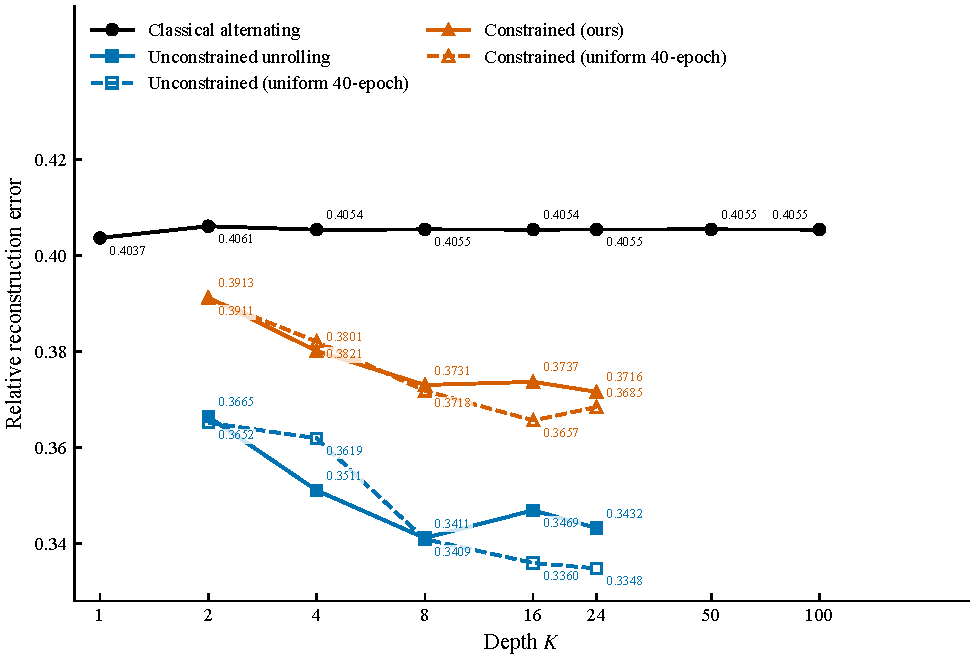
\includegraphics[width=\linewidth]{figures/fig_depth.pdf}
\caption{Test relative reconstruction error against depth $K$ on $100$ unseen noiseless samples. The frame spans the full measured range, so every arm is visible over its whole depth range. Both unrolled variants stay below the classical iteration's best value at every depth shown, and
every measured point carries its value; each archived arm and its uniform $40$-epoch replay are
offset to opposite sides of the curve, because the two coincide to within $0.003$ at $K\le8$ and
would otherwise print over one another.}
\label{fig:depth}
\end{figure}
\begin{table}[htbp]
\centering
\caption{Tuned classical baseline: best damping $\alpha=\gamma$ and the corresponding test RRE,
swept over $\alpha\in[0.1,1]$ at four depths, on 100 test samples.}
\label{tab:cls}
\begin{tabular}{lcc}
\toprule
Depth $K$ & best $\alpha=\gamma$ / RRE \\
\midrule
$8$   & $\numv{\NumClsSweepKEight}$ \\
$24$  & $\numv{\NumClsSweepKTwoFour}$ \\
$50$  & $\numv{\NumClsSweepKFifty}$ \\
$100$ & $\numv{\NumClsSweepKHundred}$ \\
\bottomrule
\end{tabular}
\end{table}
Fig.~\ref{fig:depth} shows the test RRE versus depth. The classical alternating iteration stalls
almost immediately: $\numv{\NumClassOne}$ at $K=1$, its best value over the whole range
$\numv{\NumClassBest}$ at $K=\numv{\NumClassBestK}$, and $\numv{\NumClassHundred}$ at $K=100$, 
a plateau, not a convergence. Tuning its damping does not change the picture, as Table~\ref{tab:cls} shows: even the best configuration over the whole grid is
$\numv{\NumClsSweepBest}$ (at $\numv{\NumClsSweepBestK}$), a gain of only
$\numv{\NumClsSweepGain}$ over the untuned setting. The
unrolled networks reach a comparable error in far fewer outer iterations: the
constrained network attains $\numv{\NumConsBest}$ at $K=\numv{\NumConsBestK}$ (already
$\numv{\NumConsTwo}$ at $K=2$) and the unconstrained variant $\numv{\NumUncBest}$ at
$K=\numv{\NumUncBestK}$; at $K=8$ the numbers are $\numv{\NumConsEight}$, $\numv{\NumUncEight}$
and $\numv{\NumClassEight}$ respectively. A certified $K=8$ constrained network therefore attains,
at $K=8$, an error \emph{below} the classical iteration's best value at every depth we tested
($\numv{\NumConsEight}$ against $\numv{\NumClassBest}$ at $K=\numv{\NumClassBestK}$); measured
against the classical $K=100$ run ($\numv{\NumClassHundred}$), the same network uses roughly
$12\times$ fewer \emph{outer iterations at matched per-layer cost}. The unit of comparison is the iteration
count, not wall-clock time, and the two arms are matched where it matters: both perform the same
regularized least-squares contrast solve with the same conjugate-gradient budget
($n_{\mathrm{cg}}=\numv{\NumNCg}$, Sec.~\ref{sec:exp}), so a classical step and one unrolled layer
differ only by the learned module. That module is not free: measured on the production shapes it
raises the per-layer cost to $1{+}\numv{\NumCostLayerOverhead}$ times that of a classical layer in
median wall-clock at batch $16$ (a surcharge of $\numv{\NumCostLayerOverheadPct}\%$, or
$\numv{\NumCostMacOverheadPct}\%$ in analytic multiply--accumulate counts), the correction CNN
itself accounting for $\numv{\NumCostCnnPct}\%$ of a learned layer and the CG solve for
$\numv{\NumCostCgPct}\%$ of it. A $12\times$ iteration reduction therefore
survives a per-layer surcharge of order $1.4\times$ with a wide margin, but the defensible statement is the iteration count at matched per-layer cost, which is what we report. The primary
baseline is the damped alternating fixed-point iteration, the classical ancestor of these
architectures. Two stronger classical solvers are run as well, so that the comparison does not rest on
a weak reference: contrast source inversion (CSI)~\cite{csi_lit}, which alternates the contrast source, a linear least-squares step solved by CG, with a pointwise contrast update on the classical CSI
functional, and the subspace-based optimization method (SOM)~\cite{som_lit}, which fixes the induced
current on the dominant right-singular subspace of $G_s$ from the data equation and optimises the
remainder through the state equation. Both start from the \emph{same} Born-LS initialisation as the
unrolled networks (test RRE $\numv{\NumBornInitRre}$) and are run to $K=100$ outer iterations.

SOM is a genuinely strong reference: its best test error is $\numv{\NumSomBest}$ (at
$K=\numv{\NumSomBestK}$, subspace dimension $M=\numv{\NumSomBestM}$), well below the
$\numv{\NumClsSweepBest}$ of the tuned damped iteration, so the comparison does not rest on a
weak reference. CSI improves more slowly on this problem, reaching $\numv{\NumCsiAtKEight}$ at
$K=8$ and $\numv{\NumCsiBest}$ at $K=\numv{\NumCsiBestK}$, and is beaten by the constrained
network at matched depth. Against SOM the picture is less favourable. At matched depth $K=8$ the constrained network attains $\numv{\NumConsEight}$ against
$\numv{\NumSomAtKEight}$ for SOM (best over $M$, here $M=\numv{\NumSomAtKEightM}$); the margin
$\numv{\NumSomMargKEight}$ lies \emph{below} the measured re-run floor
$\numv{\NumRepFloorMaxRre}$, so the two are indistinguishable at this depth and we claim no win.
Over the whole range SOM's best $\numv{\NumSomBest}$ is $\numv{\NumSomMargBest}$ below the
constrained network's best $\numv{\NumConsBest}$, i.e.\ SOM is the more accurate method at its
best; the certified network's contribution is that it is the only variant carrying an explicit
boundedness certificate, not that it is the most accurate. The unconstrained variant is the most
accurate of the tested methods. The subspace dimension,
like the damping of Table~\ref{tab:cls}, was selected over the grid
$M\in\{\numv{\NumSomMGrid}\}$ swept in the release. The defensible
statement is the matched-depth one, and we claim no wall-clock win, the per-layer cost
accounting below stands, only accuracy at matched outer-iteration depth. For scale, the measured
wall-clock of one complete sweep to $K=100$ on the same $100$ samples is
$\SI{\numv{\NumCsiSecHundred}}{\second}$ for CSI and
$\SI{\numv{\NumSomSecHundred}}{\second}$ for SOM at $M=6$; the unrolled arms were timed per layer
at a different batch size, so the iteration ratio is not converted into a speed-up here. The constrained curve
falls at every measured depth and saturates by $K=16$, as predicted by the depth decomposition, a geometric depth term plus a
correction floor. The $\numv{\NumDepDeltaArchPct}\%$ rise from $K=16$ to
$K=24$ that the archived curve showed is \emph{not} reproduced once every depth is trained on the
uniform schedule, where the same interval reads
$\numv{\NumDepUniConsSixteen}\!\to\!\numv{\NumDepUniConsTwentyFour}$, i.e.\
$\numv{\NumDepDeltaUniPct}\%$; we therefore no longer describe this curve as
non-monotone. That interval is in any case unresolved, for \emph{both}
arms the change is below the measured re-run floor ($\numv{\NumDepUniFloor}$, the unconstrained arm
in fact moving by $\numv{\NumDepDeltaUncUniPct}\%$ there), so our claim of saturation is a statement about \emph{resolvability}, since no change beyond $K=16$ is resolved above instrument noise, and not a strict-monotonicity claim. The unconstrained variant is more accurate at every depth at
which it was measured, by $\numv{\NumPriceDeltaLo}$--$\numv{\NumPriceDeltaHi}$
($\numv{\NumPriceDelta}$ at $K=8$), the price of the
budgets, discussed in Sec.~\ref{sec:price}. These are \emph{relative} comparisons in a controlled small-aperture setting ($8$
incidences): the absolute error floor of $\approx0.4$ is set by the mild illumination and by the
regularization of the contrast step, not by the unrolling, and is not proposed as a competitive
imaging result.

\subsection{Certified and measured spectral quantities}

\emph{Reproducibility.} Every quantity in Table~\ref{tab:cert} is produced by a single audit
driver. Its forward operator products use exact \texttt{torch.func.jvp} derivatives and its adjoints are
exact reverse-mode derivatives, both wrapped in a matrix-free operator, so no spectral estimate
is contaminated by finite-difference truncation: $\sigma_{\max}$ is obtained by Lanczos/IRAM on
$J^{\!\top}\!J$, the spectral radius by IRAM on $J$, and the transient factor $\sup_m\|J^m\|$ by
an eigenproblem on $(J^{\!\top})^mJ^m$. Power iteration is retained only as an independent
cross-check; since both estimators are rigorous lower bounds, their disagreement measures the discretisation spread rather than the value. Three \emph{exact} self-checks are reported.
(i) On a random linear test map the estimate is compared with the exact singular value returned
by \texttt{torch.linalg.matrix\_norm} (relative error $\numv{\NumInstrErr}$). (ii) On the layer
itself the measured coupling block is compared with the closed form
$\sigma_{\max}(C)=\theta\alpha\mathcal{E}$ of Lemma~\ref{lem:blocks} (measured-to-proved ratio
$\numv{\NumSigCRatio}$). (iii) In the Born variant, whose contrast step does not depend on the
field state, two blocks are analytically transparent, $\sigma_{\max}(B)\equiv0$ and
$\sigma_{\max}(A)=1-\gamma$, and the instrument reproduces both
($\numv{\NumBornSigmaB}$ and $\numv{\NumBornSigmaA}$). In the faithful variant
$\sigma_{\max}(A)$ has \emph{no} closed form, the contrast step depends on $\chi$ through the
field chain $\chi\to w^+\to E$, so there $A$ is reported as a measured quantity and never used
as a certificate. The quantities reported in Table~\ref{tab:cert}, the blocks $A$--$D$, the
full layer Jacobian and the $\alpha$-sweep, are computed in double precision, as are the
per-layer correction audit and the $\chi$-row audit; the only single-precision records in the
archive are superseded legacy files, retained for provenance and labelled as such wherever they are
cited.
The reason is that the contrast
step inverts a Tikhonov system whose smallest eigenvalue is
$\lambda_{\min}=\numv{\NumLamMin}$, so a single-precision directional derivative through the
$n_{\mathrm{cg}}=\numv{\NumNCg}$-step CG loop loses significant digits; as a recorded
illustration, at the step size where the two precisions disagree most
($\alpha=\numv{\NumPrecAlphaWorst}$) the single-precision estimator returns
$\sigma_{\max}=\numv{\NumSigSingleWorst}$ against $\numv{\NumSigDoubleWorst}$ in double precision.
The precision upgrade is itself
verifiable rather than assumed: the operators agree between the two precisions to
$\numv{\NumOpPrecRel}$, whereas one layer applied to the \emph{same} state differs by
$\numv{\NumLayerPrecAmp}$, the $\numv{\NumNCg}$-step CG solve amplifying a
$\numv{\NumOpPrecRel}$ arithmetic difference. That single-precision value is kept in the
archived results as evidence of the artefact, not used. The mapping between these derivations, the numbered statements of this paper and the functions implementing them is recorded in the repository given in the data-availability statement.
The driver provenance and row-by-row notes for Table~\ref{tab:cert} are collected in the Supplementary Material.

\begin{table}[htbp]
\centering
\caption{Blocks and thresholds of the trained layer map. ``Proved'' entries are rigorous
inequalities at the measured operating point and may serve as theorem hypotheses;
``Measured'' entries are numerical records and are \emph{not} used as hypotheses. A
dash: column not applicable to that row.}
\label{tab:cert}
\footnotesize\setlength{\tabcolsep}{4pt}
\begin{tabular}{@{}p{0.34\textwidth}p{0.20\textwidth}p{0.13\textwidth}p{0.20\textwidth}@{}}
\toprule
Block / quantity & Closed form & Proved & Measured \\
\midrule
$D$: field block $\sigma_{\max}$ of Thm.~\ref{thm:field} & $1-\alpha(1-\beta_0)=\numv{\NumGammaW}$ & $=\numv{\NumThmFieldD}$ & $\numv{\NumPhysWBlock}$ \\
$C$: coupling block of Lem.~\ref{lem:blocks} & $\alpha\mathcal{E}=\numv{\NumSigCLower}$ & $\numv{\NumSigCLower}$ & $\numv{\NumSigC}$ \\
\quad as a lower bound on $\sigma_{\max}(J)$ & $\alpha\mathcal{E}$ & $\numv{\NumSigLowBound}$ & \textemdash \\
$A$: contrast block, $\sigma_{\max}$ & \textemdash & \textemdash & $\numv{\NumSigA}$ \\
$B$: correction-side coupling, $\sigma_{\max}$ & \textemdash & \textemdash & $\numv{\NumSigB}$ \\
Peak field column norm $\mathcal{E}$ / $\ell_\infty$ ratio & $\max_r\norm{E_{\cdot,r}}_2$ & \textemdash & $\numv{\NumEColMax}$ / $\numv{\NumEInfRatio}$ \\
Non-contractivity threshold $\alpha_c=(\theta\mathcal{E})^{-1}$ & $(\theta\mathcal{E})^{-1}$ & $\numv{\NumAlphaC}$ & \textemdash \\
Physics-core $\sigma_{\max}(J)$, no correction & \textemdash & \textemdash & $\numv{\NumPhysSigma}$ \\
Born-contrast variant, forces $B\equiv0$ & \textemdash & \textemdash & $\numv{\NumBornSigmaFull}$ \\
$\operatorname{Lip}(H_k)$, slope budget $\ell$ & \textemdash & \textemdash & $\numv{\NumLipHCons}$ / $\numv{\NumLipHUnc}$ \\
\bottomrule
\end{tabular}
\end{table}

\begin{table}[htbp]
\centering
\caption{Composite, fidelity and noise quantities. All entries are measured at the trained step sizes unless the column says otherwise; the $\rho_\chi$ hypothesis of Cor.~\ref{cor:fidelity} is refuted in the unconstrained arm and left undecided in the constrained one.}
\label{tab:cert2}
\footnotesize\setlength{\tabcolsep}{4pt}
\begin{tabular}{@{}p{0.40\textwidth}p{0.14\textwidth}p{0.30\textwidth}@{}}
\toprule
Quantity & Status & Value \\
\midrule
Contrast-path blocks at the implemented solve, $A$ / $B$ / $J$ & measured & $\numv{\NumSigAImpl}$ / $\numv{\NumSigBImpl}$ / $\numv{\NumSigmaFullImpl}$ \\
Composite $\sigma_{\max}$, $K{=}8$ cyclic & measured & $\numv{\NumSigCompCons}$ / $\numv{\NumSigCompUnc}$ \\
\quad per-layer composite at fixed $\alpha=\gamma=\tfrac12$, \emph{as implemented} ($n_{\mathrm{cg}}=\numv{\NumNCg}$; converged pair $\numv{\NumGdPhysSigmaConv}$ / $\numv{\NumSigCompLayerConsConv}$) & measured & $\numv{\NumSigCompLayerCons}$ / $\numv{\NumSigCompLayerUnc}$ \\
$\rho_\chi$ = $\sigma_{\max}$ of the $\chi\!\to\!\chi$ block, a \emph{lower} bound on the $\chi$-map Lipschitz constant & measured & $\numv{\NumRhoChiCons}$ / $\numv{\NumRhoChiUnc}$ \\
\quad $\chi$-map Lipschitz constant of $\hat G$, row block $[A\,B]$ & measured & $\numv{\NumChiLipRowCons}$ / $\numv{\NumChiLipRowUnc}$ \\
\quad physical map $F$ ($H\equiv0$), row block $[A\,B]$ & measured & $\numv{\NumChiLipRowFCons}$ / $\numv{\NumChiLipRowFUnc}$ \\
\quad physical map $F$, $\chi\!\to\!\chi$ block & measured & $\numv{\NumChiFBlockCons}$ / $\numv{\NumChiFBlockUnc}$ \\
\quad physical map $F$, spectral radius, learned step sizes & measured & $\numv{\NumChiRhoFCons}$ / $\numv{\NumChiRhoFUnc}$ \\
\quad same at fixed $\alpha=\gamma=\tfrac12$ & measured & $\numv{\NumChiRhoFFixCons}$ / $\numv{\NumChiRhoFFixUnc}$ \\
\quad same block, spectral radius rather than Lipschitz constant & measured & $\numv{\NumRhoChiSpecCons}$ / $\numv{\NumRhoChiSpecUnc}$ \\
Transient $M_J=\max_{m\le2}\norm{J^m}$ (depth-2 truncation of Cor.~\ref{cor:noisenormal}) & measured & $\numv{\NumMJCons}$ \\
\quad same over the full horizon $m\in\{1,2,4,8\}$: the truncation is not benign & measured & $\numv{\NumMJFullCons}$ ($m{=}\numv{\NumMJFullArgmaxM}$) / $\numv{\NumMJFullUnc}$ ($m{=}\numv{\NumMJFullArgmaxMUnc}$) \\
Non-normality gap $\sigma_{\max}/\rho$ & measured & $\numv{\NumGapRatio}$ \\
Noise gain $\Lambda$ (data$\to\chi$ channel): field term of \eqref{eq:Lambda} & measured & $\numv{\NumLambdaMeas}$, bounded by $\numv{\NumLambdaBound}+\numv{\NumLamCorrTerm}$ \\
\bottomrule
\end{tabular}
\end{table}
\emph{Provenance.} All rows are produced by one audit driver at the Born--LS initial state, $\alpha=\gamma=1/2$ fixed, projection on, float64; the $K{=}8$ cyclic rows use a separate driver at learned step sizes. The as-implemented $n_{\mathrm{cg}}$ values differ from the converged-solve values on the contrast-path blocks only; the CG-free blocks $C$ and $D$ are bit-identical across the sweep, which is what makes the certificates CG-free. A single-precision re-run overestimates the contrast-path singular values by order one because the dominant triplet is not resolved; all tabulated values here are double precision.

Four conclusions. (1) The field block contracts at $\numv{\NumPhysWBlock}$, below the a-priori bound $1-\alpha(1-\beta_0)=\numv{\NumGammaW}$: the certificate of Theorem~\ref{thm:field} is valid but conservative. (2) The coupling block is the obstruction and it is available in closed form: $\sigma_{\max}(C)=\alpha\mathcal{E}=\numv{\NumSigCLower}>1$ with threshold $\alpha_c=\numv{\NumAlphaC}<\tfrac12$, so at the operating step size the non-contractivity is \emph{proved}, not merely observed. (3) The contrast-path blocks give $\sigma_{\max}(A)=\numv{\NumSigA}$ and $\sigma_{\max}(B)=\numv{\NumSigB}$; the $\chi$ row of $\hat G$ measures $\numv{\NumRhoChiCons}$ and $\numv{\NumChiLipRowCons}$ in the constrained arm, both below one, and $\numv{\NumChiLipRowUnc}$ in the unconstrained arm, which refutes $\rho_\chi<1$ there. Neither arm yields a certified drift radius, so Corollary~\ref{cor:fidelity} is reported as a conditional statement. (4) The composite gain exceeds one in every configuration measured, but the closed-form coupling block $\sigma_{\max}(C)=\alpha\mathcal{E}>1$ already forces $\sigma_{\max}(DT_k)>1$ for \emph{any} correction by Prop.~\ref{prop:imposs}. The bilinear coupling $\chi\odot E$ makes the faithful composite non-contractive regardless of how the correction is controlled, which is why the guarantees we offer are boundedness and layer-wise accounting rather than a per-layer contraction rate.

\subsection{Long-horizon extrapolation and the guard rails}
\label{sec:extrap}
\begin{figure}[htbp]
\centering
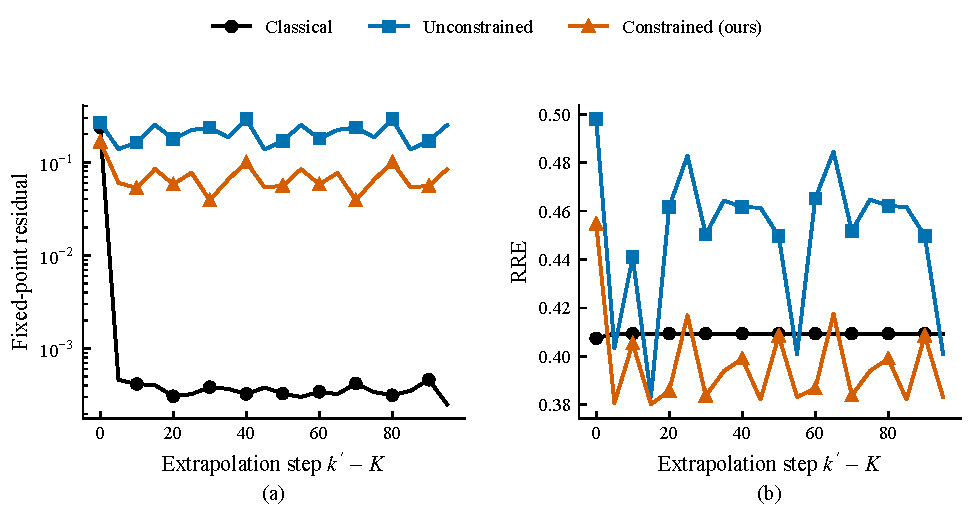
\includegraphics[width=\linewidth]{figures/fig_extrap.pdf}
\caption{Cyclic depth extrapolation of the trained $K=8$ layers ($100$ additional steps): (a) fixed-point residual; (b) reconstruction error.}
\label{fig:extrap}
\end{figure}
$\infn{\chi}$ is the largest contrast magnitude reached over the horizon; $\beta_0=\infn{\chi}\norm{\mathbf{G}_b}_2$ is the resulting a-priori constant.

\begin{figure}[htbp]
\centering
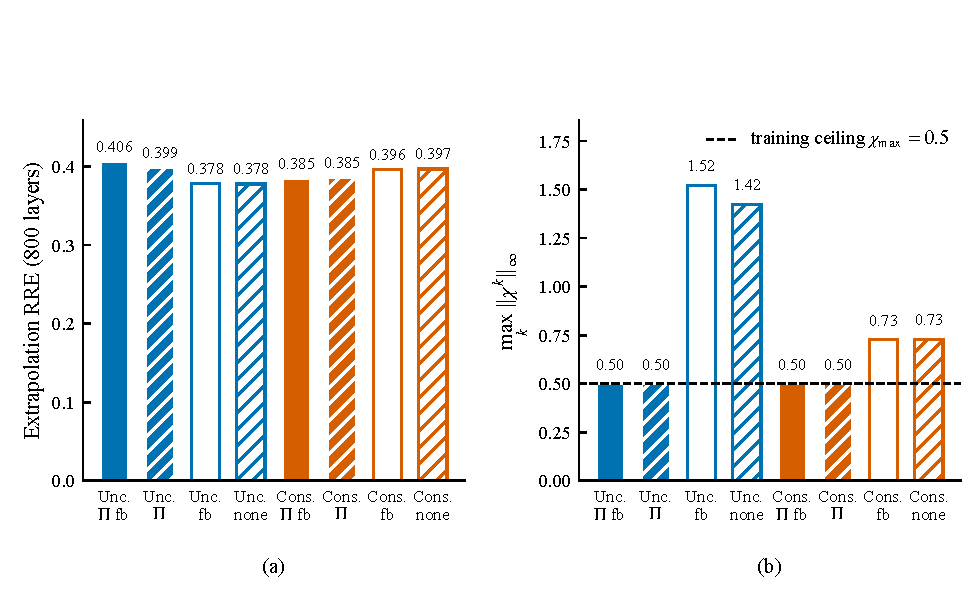
\includegraphics[width=\linewidth]{figures/fig_ablation.pdf}
\caption{Ablation~I: (a) reconstruction error and (b) trained contrast ceiling after $800$
unrolled layers, on the noiseless set of Fig.~\ref{fig:depth}. Hue gives the family,
fill the projection flag, hatching the feature bound, and the text under each bar
repeats the combination; every bar carries its value.}
\label{fig:abl}
\end{figure}
\begin{figure}[htbp]
\centering
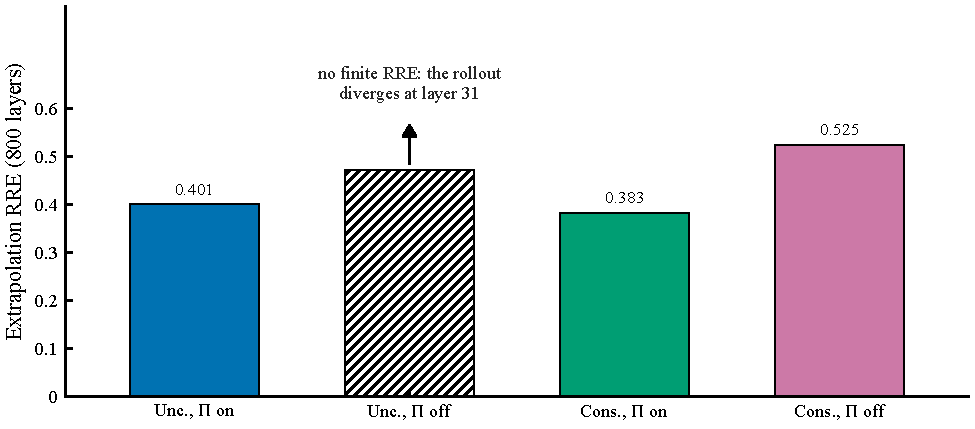
\includegraphics[width=\linewidth]{figures/fig_frozen.pdf}
\caption{Ablation~II: extrapolation error after $800$ layers with $\Pi$ removed at test time from
frozen weights, same set, linear scale. The hatched trunk is the diverging run, its top
deliberately not a value; the numbers on the other columns are the tabulated errors.}
\label{fig:frozen}
\end{figure}
Fig.~\ref{fig:extrap} repeats the trained $K=8$ layers cyclically for $100$ additional steps
($800$ layers total). Neither unrolled network contracts monotonically. The constrained
residual falls from $\numv{\NumResConsTrans}$ at the first step into a narrow limit cycle and
then oscillates within $[\numv{\NumResConsBandLo},\numv{\NumResConsBandHi}]$ for the remaining
horizon --- $\numv{\NumResConsHead}$ at a representative step, $\numv{\NumResConsEnd}$ at the last recorded step, the record being sampled every five steps ---
with $\infn{\chi}$ pinned at $\numv{\chimax}$, so its reconstruction error stays bounded. The unconstrained residual is \emph{not} monotone either,
and quoting its endpoints would understate it: it spikes to $\numv{\NumResUncSpike}$ inside the
cycle, more than an order of magnitude above the constrained band, while $|\chi|$ is still
clamped by $\Pi$. The drift is therefore visible in the residual, not in the state; the
classical iteration sits at its own fixed point
(residual $\approx\numv{\NumResClsEnd}$).

\begin{table}[htbp]
\centering
\caption{Ablation~I: complete $2\times2\times2$ factorial over the training-time flags, run for
$800$ unrolled layers; apart from the listed flags the seed and the training schedule
are identical. A dash marks a flag that does not apply to that arm.}
\label{tab:abl}
\begin{tabular}{llcccc}
\toprule
Corr. & $\Pi$ & feat. bd. & Extrap. RRE & $\infn{\chi}$ & $\beta_0$ \\
\midrule
classical & --- & --- & $\numv{\NumAblClsProjOn}$ & $\numv{\NumAblClsChi}$ & $\numv{\betacert}$ \\
unc.  & on  & on  & $\numv{\NumAblUncPOnFbOnRre}$ & $\numv{\NumAblUncPOnFbOnChi}$ & $\numv{\NumBetaUncPOnFbOn}$ \\
unc.  & on  & off & $\numv{\NumAblUncPOnFbOffRre}$ & $\numv{\NumAblUncPOnFbOffChi}$ & $\numv{\NumBetaUncPOnFbOff}$ \\
unc.  & off & on  & $\numv{\NumAblUncPOffFbOnRre}$ & $\numv{\NumAblUncPOffFbOnChi}$ & $\numv{\NumBetaUncPOffFbOn}$ \\
unc.  & off & off & $\numv{\NumAblUncPOffFbOffRre}$ & $\numv{\NumAblUncPOffFbOffChi}$ & $\numv{\NumBetaUncPOffFbOff}$ \\
cons. & on  & on  & $\numv{\NumAblConsPOnFbOnRre}$ & $\numv{\NumAblConsPOnFbOnChi}$ & $\numv{\NumBetaConsPOnFbOn}$ \\
cons. & on  & off & $\numv{\NumAblConsPOnFbOffRre}$ & $\numv{\NumAblConsPOnFbOffChi}$ & $\numv{\NumBetaConsPOnFbOff}$ \\
cons. & off & on  & $\numv{\NumAblConsPOffFbOnRre}$ & $\numv{\NumAblConsPOffFbOnChi}$ & $\numv{\NumBetaConsPOffFbOn}$ \\
cons. & off & off & $\numv{\NumAblConsPOffFbOffRre}$ & $\numv{\NumAblConsPOffFbOffChi}$ & $\numv{\NumBetaConsPOffFbOff}$ \\
\bottomrule
\end{tabular}
\end{table}
\begin{table}[htbp]
\centering
\caption{Ablation~II, inference-time removal of $\Pi$ from \emph{frozen} weights trained
\emph{with} $\Pi$ ($K=8$; ``RRE'' short-horizon / $800$-layer extrapolation).
``div.'' marks a rollout that left the finite range before the horizon, so it has no
extrapolation error to quote.}
\label{tab:abl2}
\begin{tabular}{llccc}
\toprule
Frozen weights & $\Pi$ at test & RRE short & RRE extrap. & $\infn{\chi}$ \\
\midrule
unconstrained & on  & $\numv{\NumFrzUncOnShort}$ & $\numv{\NumFrzUncOn}$ & $\numv{\chimax}$ \\
unconstrained & off & $\numv{\NumFrzUncOffShort}$ & $\numv{\NumFrzUncOff}$ & $\numv{\NumFrzUncOffChi}$ \\
constrained   & on  & $\numv{\NumFrzConsOnShort}$ & $\numv{\NumFrzConsOn}$ & $\numv{\chimax}$ \\
constrained   & off & $\numv{\NumFrzConsOffShort}$ & $\numv{\NumFrzConsOff}$ & $\numv{\NumFrzConsOffChi}$ \\
\bottomrule
\end{tabular}
\end{table}
\noindent
Tables~\ref{tab:abl}--\ref{tab:abl2} show which ingredient is responsible for which property.
Each component is read off the quantity that carries its theoretical role, not off a single error
column: the projection through the contrast ceiling $\infn{\chi}$, which is pinned at $\chi_{\max}$
in every arm that has it and leaves the box in every arm that does not; the amplitude budget
through the realised correction relative to $\bar\epsilon$; the feature bound through the trunk
input range that makes $\bar\epsilon$ attainable at all; the spectral clamp through the module
norm, and negatively, through the absence of a stability gain at fixed budget; and the CG budget
through the residual and the block drift recorded in Supplementary Material, Sec.~1.
The two tables answer \emph{different} questions and are not two estimates of one effect.
Ablation~II holds the weights fixed and removes $\Pi$ at inference time --- same initial state,
same $K{=}8$ block repeated to $800$ layers, no retraining --- so it isolates what the projection
does to a trajectory that was trained with it. Ablation~I retrains every arm from scratch with
$\Pi$ switched off and asks whether training can find a stable parameter set without it. A bounded
outcome in the second is an empirical property of the parameter set that training landed on and
carries no a-priori certificate; the two are therefore never pooled into a single claim about the
necessity of the projection.

\emph{(a) The projection is indispensable at inference time.} Ablation~II, tabulated in Table~\ref{tab:abl2} and plotted in Fig.~\ref{fig:frozen}, removes $\Pi$ from \emph{frozen} weights that were
trained with it, the cleanest possible single-variable test. The
unconstrained network's error jumps from $\numv{\NumFrzUncOn}$ to
$\numv{\NumFrzUncOffShort}$ already at the short horizon, and its $800$-layer rollout leaves the
finite range at layer $\numv{\NumFrzUncBreak}$, with $\infn{\chi}$ reaching
$\numv{\NumFrzUncOffChi}$: the state leaves the admissible set by two orders of magnitude and the
iterate does not return. The constrained network
degrades but survives ($\numv{\NumFrzConsOff}$), because its correction is bounded by
$\bar\epsilon$ and cannot push the state far. This is the operational statement of
Theorem~\ref{thm:bounded}: the projection is not a cosmetic clamp.

\emph{(b) Retraining can hide the problem, but only at the cost of the certificate.} Ablation~I, tabulated in Table~\ref{tab:abl} and plotted in Fig.~\ref{fig:abl}, shows that a network \emph{trained} without $\Pi$
re-learns an operating point that happens to
stay bounded ($\numv{\NumAblUncPOffFbOnRre}$ versus $\numv{\NumAblUncPOnFbOnRre}$ with $\Pi$, a
difference of $\numv{\NumAblProjDelta}$). The classical row of Table~\ref{tab:abl} has no learned correction, no projection flag and no feature-bound flag, and since its contrast saturates the ceiling $\chi_{\max}=\numv{\chimax}$ its $\beta_0$ is the certified $\chi_{\max}\norm{\mathbf{G}_b}_2=\numv{\betacert}$ rather than a separately measured value. What it does not keep is the bound: the measured
$\infn{\chi}=\numv{\NumAblUncPOffFbOnChi}$ gives $\beta_0^{\mathrm{meas}}=\numv{\NumBetaMeas}>1$, so
the hypothesis of Theorem~\ref{thm:bounded} fails and boundedness reverts to an empirical
observation about one trained parameter set. This is exactly the distinction the unrolling
literature currently does not make, and it is the practical reason to keep $\Pi$:
\emph{boundedness by luck versus boundedness by construction}.

\emph{(c) What the guard rails actually buy, a negative result about error as a proxy.} No
arm leaves the floating-point range: all eight are numerically finite over the whole horizon.
The arms are separated by the \emph{state}, not by the error. With $\Pi$ on, $\infn{\chi}$ is pinned
at $\numv{\chimax}$ in every arm; with $\Pi$ off it reaches
$\numv{\NumAblUncPOffFbOnChi}$--$\numv{\NumAblUncPOffFbOffChi}$, i.e.\ it leaves the admissible
box while the reconstruction error stays finite, and is in fact slightly \emph{lower}: $\numv{\NumAblUncPOffFbOnRre}$ against $\numv{\NumAblUncPOnFbOnRre}$, a single-variable comparison in the projection with feature bounding held on. A finite error is
therefore \emph{not} evidence of the certificate: the certificate is a statement about the
state, and it is the projection, not the observed accuracy, that enforces it. We report this
explicitly because the opposite reading, ``the unconstrained rollout diverges'', is what
the earlier unrolling literature reports and what a reader would expect here, and it is not
what our data show. Feature bounding remains load-bearing for a different reason: it is what
makes the amplitude budget $\bar\epsilon$ attainable by construction, as Remark~\ref{rem:featscale} explains.

\emph{(d) The boundedness reading is not a single-run artefact.} The arms above are reported for one
training seed, so we replicated the contrast they rest on over
$\numv{\NumSeedNCons}$ training seeds per arm ($\numv{\NumSeedNCons}$ constrained,
$\numv{\NumSeedNUnc}$ unconstrained, $\numv{\NumSeedNProjOff}$ unconstrained with the projection
removed), each seed a full retrain with its own data and initialization seed. Every run stays
numerically finite ($\numv{\NumSeedFinite}$). The constrained arms sit at
$\infn{\chi}=\numv{\NumSeedChiConsMax}$, pinned at the box, in \emph{every} seed, while the
arms trained without the projection leave it in every seed
($\infn{\chi}=\numv{\NumSeedProjOffBox}$); the separation is therefore a property of the design
flag, not of one initialization. The depth conclusion is equally stable: over these runs the
$K{=}8$ test error is $\numv{\NumSeedRreMeanCons}\pm\numv{\NumSeedRreSdCons}$ (constrained) and
$\numv{\NumSeedRreMeanUnc}\pm\numv{\NumSeedRreSdUnc}$ (unconstrained), where the second term is
the population standard deviation and the dispersion is not carried by the mean alone: the
medians are $\numv{\NumSeedRreMedCons}$ and $\numv{\NumSeedRreMedUnc}$ and the upper quartiles
$\numv{\NumSeedRreHiCons}$ and $\numv{\NumSeedRreHiUnc}$, so no run hides in a tail. The
$800$-layer extrapolation error over the same runs is
$\numv{\NumSeedExMeanCons}\pm\numv{\NumSeedExSdCons}$ and
$\numv{\NumSeedExMeanUnc}\pm\numv{\NumSeedExSdUnc}$. That standard deviation must be read with care, because the quantity it is usually mistaken for was measured as well. Re-running the \emph{same} driver at the
\emph{same} seeds, the training path is byte-identical between the two archives, moves
the $K{=}8$ error by up to $\numv{\NumRepFloorMaxRre}$ (median $\numv{\NumRepFloorMedRre}$) and the
$800$-layer extrapolation error by up to $\numv{\NumRepFloorMaxExtrap}$, over the
$\numv{\NumRepNShared}$ runs present in both archives. The identical-seed floor is therefore
\emph{not} small compared with the across-seed spread, and we do not present the latter as an error
bar on this pipeline. What the replication establishes is narrower: the two verdicts the conclusion rests on are unchanged in every repeat, every run is numerically finite, and the admissible-box
verdict is stable in all $\numv{\NumRepNShared}$ overlapping runs
(finite-stable: \numv{\NumRepFiniteStable}; box-stable: \numv{\NumRepBoxStable}).

The practical recommendation is consequently stronger than ``project if convenient'': the
projection plus a bounded feature map are the two ingredients that convert unrolled inverse
scattering from an empirically stable heuristic into an iteration with a closed-form invariant
set; the amplitude budget then supplies the fidelity radius of Corollary~\ref{cor:fidelity}.

\subsection{Noise stability}\label{sec:noise}

\emph{Noise protocol.} Training samples carry complex Gaussian
noise. Its SNR is $\SI{20}{\decibel}$, defined as ten times the base-10 logarithm of the mean
noiseless signal power $\mean|y^{0}|^{2}$ over the mean noise power $\mean|n|^{2}$, so that the
ratio is averaged over all receiver and incidence channels; the evaluation set ($100$ unseen samples) is
noiseless by construction, so that the depth and extrapolation studies measure reconstruction error
and not measurement noise; noise is injected explicitly below at
$\SI{30}{\decibel}$--$\SI{5}{\decibel}$. ``Noiseless'' here means the synthesis SNR is set to
$\SI{\numv{\NumNoiseNominalDb}}{\decibel}$, and we do not take that number at face value: the
generator computes in float64 but \emph{delivers} the field as complex64, so the quietest signal the
stored data can represent is the complex64 representation error. We measure it
($\numv{\NumNoiseFloorRel}$ in relative norm, an effective floor at
$\SI{\numv{\NumNoiseFloorDb}}{\decibel}$), so the evaluation set is noiseless only in the sense that
its measured floor lies far below the $\SI{30}{\decibel}$--$\SI{5}{\decibel}$ noise injected later;
we quote that floor rather than the requested value.
The solid markers are computed at a \emph{converged} contrast solve ($n_{\mathrm{cg}}=\numv{\NumNCgConv}$), matching Table~\ref{tab:cert}; the faint grey series is the as-implemented $n_{\mathrm{cg}}=\numv{\NumNCg}$ sweep, retained only as the record of the artefact discussed in Sec.~\ref{sec:exp}. Fig.~\ref{fig:alphac} plots that sweep: it comprises $\numv{\NumAlphaSweepN}$ values of $\alpha=\gamma$ spanning $[0.05,1]$, and $\mathcal{E}=\max_r\norm{E_{\cdot,r}}_2$ is tabulated in Table~\ref{tab:cert}, so $\alpha_c=(\theta\mathcal{E})^{-1}$ is recomputable from the tabulated quantities alone.

\begin{figure}[htbp]
\centering
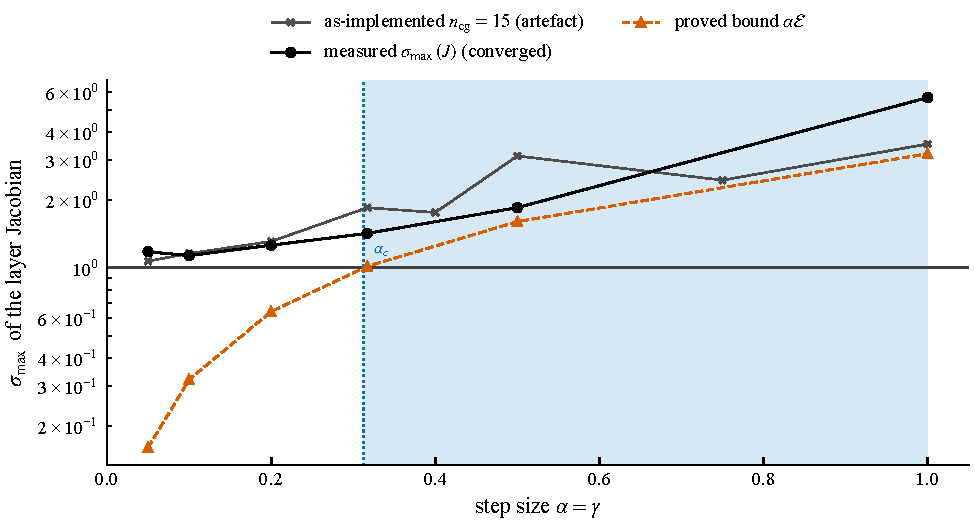
\includegraphics[width=\linewidth]{figures/fig_alphac.pdf}
\caption{Measured $\sigma_{\max}$ of the physics-core layer Jacobian versus step size $\alpha=\gamma$ (markers), against the rigorous lower bound $\alpha\mathcal{E}$ of Prop.~\ref{prop:imposs} (dashed) and the threshold $\alpha_c=(\theta\mathcal{E})^{-1}$ (dotted). Only the region right of $\alpha_c$ is proved.}
\label{fig:alphac}
\end{figure}
\begin{figure}[htbp]
\centering
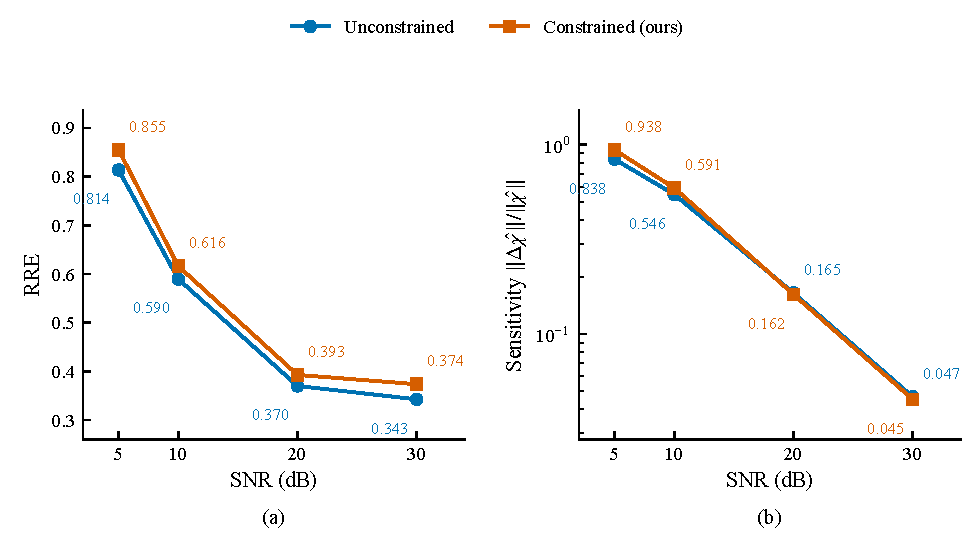
\includegraphics[width=\linewidth]{figures/fig_noise.pdf}
\caption{Noise sensitivity at depth $K=8$: (a) reconstruction error versus SNR;
(b) output perturbation $\norm{\hat\chi(y+\Delta y)-\hat\chi(y)}/\norm{\hat\chi(y)}$
on 100 test samples per point. Every marker carries its value.}
\label{fig:noise}
\end{figure}
Fig.~\ref{fig:noise} evaluates both networks under measurement noise from $\SI{30}{\decibel}$
down to $\SI{5}{\decibel}$. Both degrade monotonically, and their sensitivities
$\numv{\NumSensCons}$ (constrained) versus $\numv{\NumSensUnc}$ (unconstrained) at
$\SI{20}{\decibel}$ are close: in this experiment the amplitude budget does \emph{not} buy a
visible noise advantage. What the budget supplies is not a bound of the form $\Lambda/(1-\rho)$,
which as shown above is conditional and has a false hypothesis here, but the \emph{quantities}
$\Lambda$ and $M_J$ entering the exact accounting \eqref{eq:noiseexact}; these are recomputable for
any grid and can be tracked across training. We report this as an explicit negative empirical
finding: the value of the constrained family is certifiability and boundedness, not accuracy or
measured robustness, and a noise guarantee for this architecture would require either the averaged
construction of Remark~\ref{rem:averaged}, with its accuracy cost, or a depth-bounded deployment
with the measured $\Lambda$ and $M_J$.

\subsection{Per-layer gains and gradients}
These are contrast-path quantities, computed by power iteration on the realified Jacobian and validated against exact SVD on linear test maps.

\begin{figure}[htbp]
\centering
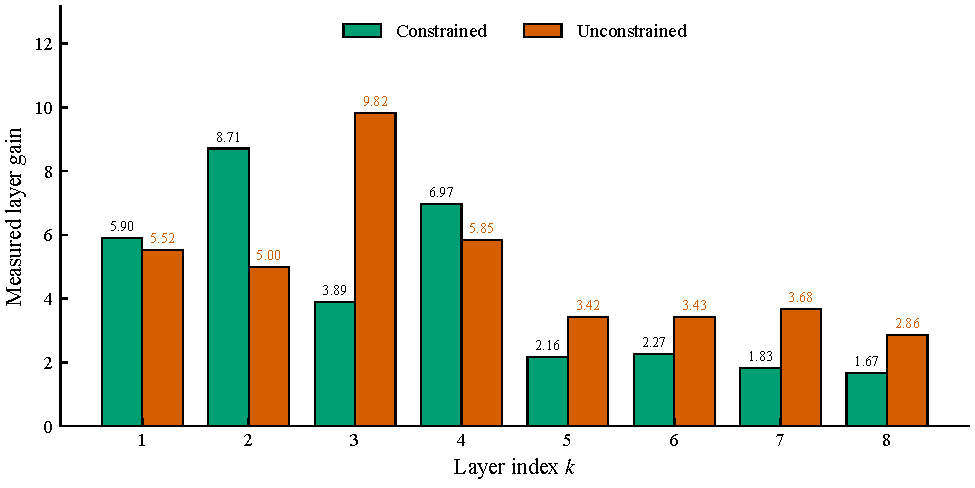
\includegraphics[width=\linewidth]{figures/fig_gain.pdf}
\caption{Measured spectral norm of each layer's Jacobian at the learned step sizes, on the as-
implemented contrast path ($n_{\mathrm{cg}}=\numv{\NumNCg}$), with the value printed on
every bar.}
\label{fig:gain}
\end{figure}
The first-layer gradient norm versus truncated backward-pass depth, for the $K=24$ models, is
reported in Supplementary Material, Fig.~S2.
At the \emph{learned} step sizes, plotted in Fig.~\ref{fig:gain}, both variants exceed one at every layer,
with the constrained variant not systematically smaller, the composite gain is dominated by the
physics core, whose damping factors $\alpha_k$ are themselves learned and, in the constrained run,
converge to larger values ($\numv{\NumAlphaCons}$ versus $\numv{\NumAlphaUnc}$). This is a
confounded comparison; Table~\ref{tab:cert} removes the confound by fixing
$\alpha=\gamma=0.5$. The gradient-norm probe in Supplementary Material, Fig.~S2, shows the training-side
counterpart of the budget: the first-layer gradient norm is $\numv{\NumGradConsOne}$ under the
budgets versus $\numv{\NumGradUncOne}$ without them at truncated depth $1$, and both decay with
depth, a vanishing-gradient effect that is intrinsic to deep unrolling and that the
constrained parameterization amplifies by suppressing the effective step size. This is the
gradient-health price of the guarantees.

\subsection{The price of certification}\label{sec:price}
\begin{figure}[htbp]
\centering
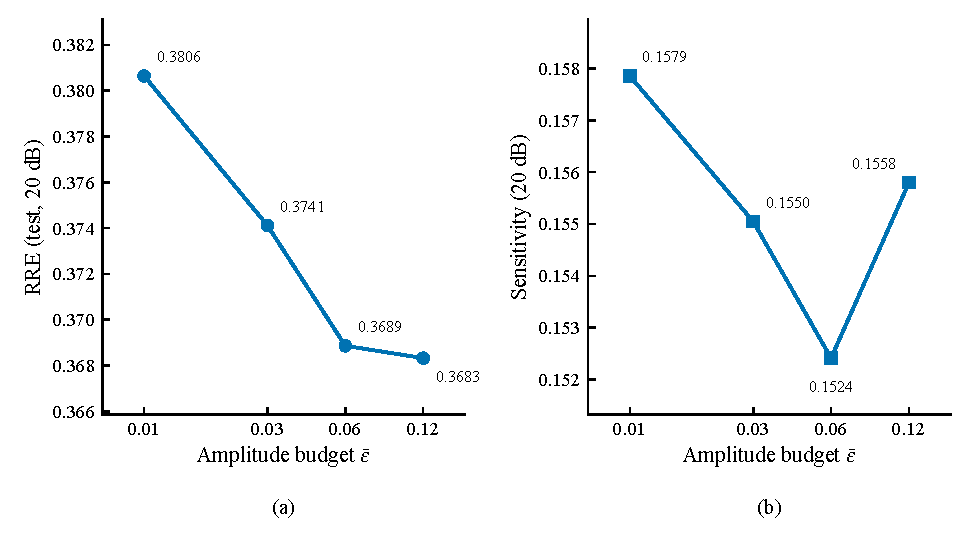
\includegraphics[width=\linewidth]{figures/fig_pareto.pdf}
\caption{Amplitude-budget sweep at $K=8$ over a factor of twelve in $\bar\epsilon$, drawn at the
swept budgets on a logarithmic axis: (a) accuracy, (b) noise sensitivity.}
\label{fig:pareto}
\end{figure}
\begin{figure}[htbp]
\centering
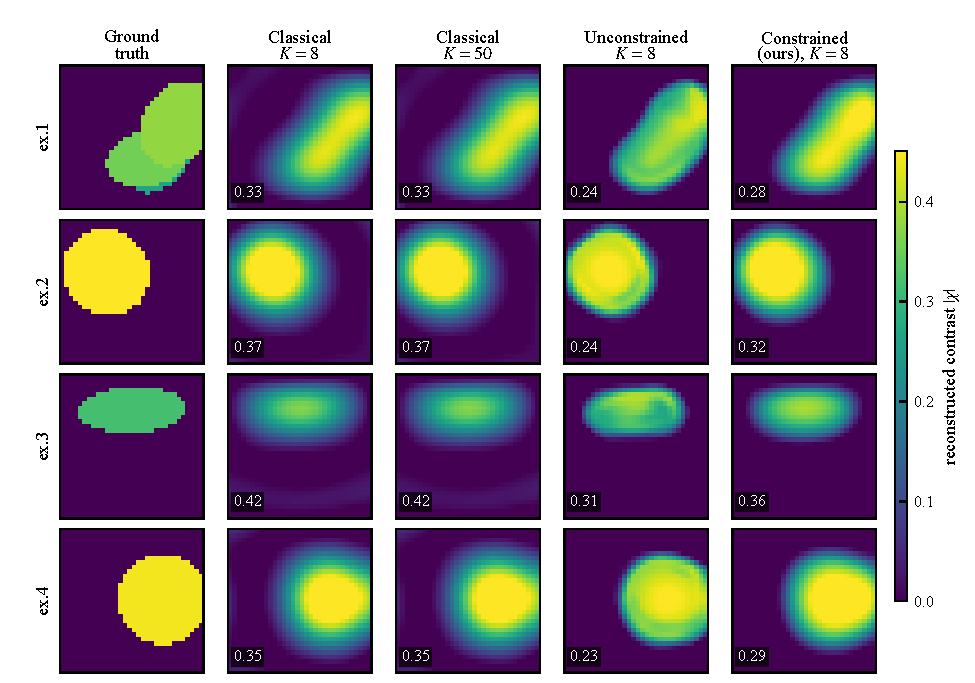
\includegraphics[width=\linewidth]{figures/fig_images.pdf}
\caption{Reconstruction examples from the test set at one colour scale. The number in each panel
is that panel's relative error $\|\hat\chi-\chi\|_2/\|\chi\|_2$ (smaller is better), not a squared
error, so the visual comparison is also a measurement. Each heading gives the method and its
depth. The two learned arms differ in the amplitude budget, not in the projection; the
text attributes the gap between their numbers.}
\label{fig:images}
\end{figure}
Fig.~\ref{fig:pareto} sweeps $\bar\epsilon$ at $K=8$. Both the error and the sensitivity improve
as $\bar\epsilon$ is increased from $\numv{\NumEbWorst}$ to $\numv{\NumEbBest}$: within the
budgeted family the constraint is a \emph{floor}, not an optimizer, and the default
$\bar\epsilon=\numv{\epsbar}$ sits in the flat part of the curve. The relevant trade-off is not
inside the constrained family but between that family and unconstrained unrolling: the accuracy
gap $\numv{\NumPriceDelta}$ of Fig.~\ref{fig:depth} is what one pays for the boundedness
certificate of Theorem~\ref{thm:bounded} and the field-subsystem rate of
Theorem~\ref{thm:field}, together with the audit of Tables~\ref{tab:abl}--\ref{tab:abl2}. Stated
plainly: unconstrained unrolling is the better estimator, the constrained family is the better
\emph{artifact}, it comes with a warranty, and the warranty is boundedness plus recomputable
constants, not a contraction rate by Prop.~\ref{prop:imposs}. Fig.~\ref{fig:images} shows test
reconstructions. One feature of that figure is easy to misread. The number in each panel is a
distance, so smaller is better, and on every example the constrained arm's number is the larger
of the two ($\numv{\NumRreImgCons}$ against $\numv{\NumRreImgUnc}$ on these four panels,
$\numv{\NumConsEight}$ against $\numv{\NumUncEight}$ on the full test set). That is neither a
sign convention nor an effect of the projection. In the factorial of
Table~\ref{tab:abl} at $K=8$ the amplitude budget accounts for $+\numv{\NumPriceBudget}$ of the
gap, while switching the projection off moves the error by $-\numv{\NumPriceProjUnc}$ in the
unconstrained arm and $+\numv{\NumPriceProjCons}$ in the constrained one, i.e.\ with no
consistent sign. The gap is the measured price of the budget $\bar\epsilon$ itself, that is, of
the parameter which makes the invariant set of Theorem~\ref{thm:bounded} explicit; it buys no
accuracy and is not presented as one.
As an image-domain check that does not
pass through the relative contrast error, we additionally measure PSNR and SSIM on the
$\numv{\NumNImg}$ examples displayed in Fig.~\ref{fig:images}: the constrained network attains
$\numv{\NumPsnrCons}$~dB / SSIM~$\numv{\NumSsimCons}$, the unconstrained network
$\numv{\NumPsnrUnc}$~dB / SSIM~$\numv{\NumSsimUnc}$, and the classical $K=8$ and $K=50$ iterations
$\numv{\NumPsnrClsEight}$ and $\numv{\NumPsnrClsFiveZero}$~dB with SSIM~$\numv{\NumSsimClsEight}$ and
$\numv{\NumSsimClsFiveZero}$. The ordering agrees with the full-test-set relative error of
Fig.~\ref{fig:depth}, and the classical $K=50$ iteration is \emph{worse} on both image metrics than
$K=8$, the plateau of Fig.~\ref{fig:depth} seen in the image domain. Two caveats are part of the
claim: these two metrics are computed on the $\numv{\NumNImg}$ displayed examples only, not on the
full test set over which every relative error in this paper is quoted, so the corresponding
subset relative errors differ from the full-set values ($\numv{\NumRreImgCons}$ and
$\numv{\NumRreImgUnc}$ here, versus $\numv{\NumConsEight}$ and $\numv{\NumUncEight}$ on the full
set); and PSNR is normalised by the contrast range of the ground truth, not by an image-intensity
convention.

\subsection{Certificate boundary under elevated contrast}
\label{sec:contrast}

\begin{table}[htbp]
\centering
\caption{The certificate boundary under elevated contrast ceilings $\chi_{\max}$, on a fixed test
geometry. RRE is quoted at the trained depth $K=8$ and the state extrema over a
$100$-layer rollout; cycle gain and the field certificate are power-iteration estimates.
``Not run'': projection-off arm not executed at that ceiling.}
\label{tab:contrast}
\small
\setlength{\tabcolsep}{4pt}
\begin{tabular}{lcccccc}
\toprule
$\chi_{\max}$ & $\beta_0^{\mathrm{meas}}$ & RRE, $K=8$ & $\max\|w\|_\infty$, proj.\ on & cycle gain & \shortstack{$\sup_k\sigma_{\max}$\\$\mathrm{diag}(\chi^k)\mathbf G_b$\\proj.\ on} & $\max|\chi|$, proj.\ off \\
\midrule
0.5  & \numv{\NumBetaZeroFive}  & \numv{\NumRreZeroFive}  & \numv{\NumMaxWZeroFive}  & \numv{\NumCycGainZeroFive}  & \numv{\NumFieldSubCertZeroFive}  & not run \\
0.75 & \numv{\NumBetaSevenFive} & \numv{\NumRreSevenFive} & \numv{\NumMaxWSevenFive} & \numv{\NumCycGainSevenFive} & \numv{\NumFieldSubCertSevenFive} & not run \\
1.0  & \numv{\NumBetaOneZero}  & \numv{\NumRreOneZero}  & \numv{\NumMaxWOneZero}  & \numv{\NumCycGainOneZero}  & \numv{\NumFieldSubCertOneZero}  & \numv{\NumProjOffChiOneZero} \\
1.5  & \numv{\NumBetaOneFive}  & \numv{\NumRreOneFive}  & \numv{\NumMaxWOneFive}  & \numv{\NumCycGainOneFive}  & \numv{\NumFieldSubCertOneFive}  & \numv{\NumProjOffChiOneFive} \\
\bottomrule
\end{tabular}
\end{table}

Table~\ref{tab:contrast} and the depth sweeps of this subsection probe the boundary of the
field-subsystem certificate on target shapes that are identical across ceilings: the test data
are generated with the same seed so that only the contrast magnitude $\chi_{\max}$ is scaled.
The a-priori certificate of Theorem~\ref{thm:field} requires
$\beta_0=\chi_{\max}\norm{\mathbf{G}_b}_2<1$. The measured value is
$\numv{\NumBetaZeroFive}$ at the in-distribution ceiling $\chi_{\max}=\numv{\NumMaxChiBox}$, and it
rises above the threshold as soon as the ceiling is raised: $\numv{\NumBetaSevenFive}$,
$\numv{\NumBetaOneZero}$ and $\numv{\NumBetaOneFive}$ at $\chi_{\max}=0.75$, $1.0$ and $1.5$. The
certificate therefore fails outside the trained range exactly where its hypotheses say it must,
and the measured boundary is the object of this experiment rather than a claim that the boundary
is unreachable.

With the projection on, the states remain bounded at every depth up to $100$ layers at every
ceiling: the reconstructed contrast is pinned at the box $\max|\chi|=\numv{\NumMaxChiBox}$ and
the field norm saturates at $\max\|w\|_\infty\le\numv{\NumMaxWOneFive}$ instead of diverging. The
confinement is not delivered by Theorem~\ref{thm:bounded}, whose a-priori hypothesis fails as soon
as the ceiling is raised: $\beta_0^{\mathrm{meas}}=\numv{\NumBetaZeroFive}<1$ at the
in-distribution ceiling but $\numv{\NumBetaSevenFive}$, $\numv{\NumBetaOneZero}$ and
$\numv{\NumBetaOneFive}$ above it. The field subsystem nonetheless contracts along the trajectory.
The Jacobian of the damped field step is $J_w=(1-\alpha)I+\alpha\,\mathrm{diag}(\chi)\mathbf G_b$,
so the trajectory quantity $\sup_k\norm{\mathrm{diag}(\chi^k)\mathbf G_b}_2$ is the empirical
counterpart of $\beta_0$ that Theorem~\ref{thm:field} bounds a priori; measured along the same
rollout it is $\numv{\NumFieldSubCertZeroFive}$, $\numv{\NumFieldSubCertSevenFive}$,
$\numv{\NumFieldSubCertOneZero}$ and $\numv{\NumFieldSubCertOneFive}$ at the four ceilings (last
column of Table~\ref{tab:contrast}), below one throughout---including at the three ceilings where
$\beta_0^{\mathrm{meas}}$ exceeds one---because the projection pins $\chi^k$ at the box and the
ceiling contrast that enters $\beta_0$ is never realised on the rollout. The comparison is causal:
the same weights with the projection switched off diverge, to $\max|\chi|=\numv{\NumProjOffChiOneZero}$ and
$\max\|w\|_\infty=\numv{\NumProjOffWOneZero}$ at $\chi_{\max}=1.0$ and to
$\numv{\NumProjOffChiOneFive}$ and $\numv{\NumProjOffWOneFive}$ at $\chi_{\max}=1.5$ after $100$ layers.

The price of the certificate is fidelity, and the degradation is truncation-dominated. The
fraction of ground-truth cells above the box grows from zero at the in-distribution ceiling to
$\numv{\NumFracBoxSevenFive}$, $\numv{\NumFracBoxOneZero}$ and $\numv{\NumFracBoxOneFive}$ as the ceiling is
raised, the network cannot represent contrast outside the box, and RRE at the trained depth
degrades from $\numv{\NumRreZeroFive}$ to $\numv{\NumRreSevenFive}$, $\numv{\NumRreOneZero}$ and
$\numv{\NumRreOneFive}$. Non-contraction strengthens with contrast: the cyclic composite gain rises
from $\numv{\NumCycGainZeroFive}$ to $\numv{\NumCycGainOneFive}$, a factor of roughly $22.5$. Noise
sensitivity grows in the same direction, with the relative gain at $20$~dB rising from
$\numv{\NumSensZeroFive}$ to $\numv{\NumSensOneFive}$. The measured conclusion is threefold: the
certificate boundary lies where the theory places it, the projection independently guarantees
boundedness beyond that boundary, and the cost of the guarantee is a truncation-limited estimate
rather than instability.

\emph{Ceiling ladder.} Table~\ref{tab:contrast} holds the weights fixed and raises what the
targets carry. The complementary experiment moves the training distribution with the box: both
arms are retrained at $\chi_{\max}\in\{0.6,0.8,1.0\}$ on data from the same generator, the same
seeds and the same $K=8$, $40$-epoch schedule, with the ceiling as the only changed parameter.
The a-priori gate is crossed almost immediately. Since
$\beta_0=\chi_{\max}\norm{\mathbf{G}_b}_2$ with $\norm{\mathbf{G}_b}_2=\numv{\NumBoxGb}$, the gate
evaluates to $\beta_0=\numv{\NumBoxBetaSixty}$, $\numv{\NumBoxBetaEighty}$ and
$\numv{\NumBoxBetaHundred}$ at
the three ceilings, so the field-subsystem certificate survives the first rung with a margin below
half a percent and is out of scope from $\chi_{\max}=0.8$ on; the crossing is at
$\chi_{\max}=\numv{\NumBoxEdge}$, about a fifth above the ceiling we trained at. What does
\emph{not} move is as informative. The non-contractivity threshold $\alpha_c=(\theta\mathcal{E})^{-1}$
contains no $\chi_{\max}$ at all, so Prop.~\ref{prop:imposs} is ceiling-free. The projection keeps
every rollout inside its box ($\max|\chi|=\numv{\NumBoxChiConsSixty}$,
$\numv{\NumBoxChiConsEighty}$ and $\numv{\NumBoxChiConsHundred}$ over $800$ layers, i.e.\ the
clamp is active rather than slack) and all $\numv{\NumBoxRuns}$ rollouts stay numerically finite;
this is the same division of labour the Fresnel geometry shows at
$\beta_0=\numv{\NumFresnelBeta}$, boundedness from the projection and a rate only from
$\beta_0$. Accuracy degrades mildly and in the same direction in both arms (constrained
$\numv{\NumBoxRreConsSixty}\to\numv{\NumBoxRreConsEighty}\to\numv{\NumBoxRreConsHundred}$,
unconstrained $\numv{\NumBoxRreUncSixty}\to\numv{\NumBoxRreUncEighty}\to\numv{\NumBoxRreUncHundred}$),
which places the degradation of Table~\ref{tab:contrast} in the targets rather than in
transporting in-distribution weights outside their range. The hierarchy of guarantees therefore
stands as a function of the ceiling: one statement is ceiling-free, one is the projection's, and
only the contraction certificate has a numerical domain, whose edge is
$\chi_{\max}=\numv{\NumBoxEdge}$ on this grid.

\subsection{Cross-geometry generalization}
\label{sec:geom}

\begin{table}[htbp]
\centering
\caption{Cross-geometry evaluation at the trained depth $K=8$ over a $100$-layer rollout. The
families are ellipses or rings, rotated rectangles with sharp corners, full-span bands,
and irregular contours from angular-modulated radial profiles; training and test
instances are isolated by seed.}
\label{tab:geom}
\small
\setlength{\tabcolsep}{4pt}
\begin{tabular}{lcccc}
\toprule
family & $\beta_0^{\mathrm{meas}}$ & RRE, rect-trained & RRE, ellipse-trained & max $\|w\|_\infty$ at depth $100$ \\
\midrule
ellipses or rings & \numv{\NumBetaGeomEll}    & \numv{\NumRreRectEll}    & \numv{\NumRreEllEll}    & \numv{\NumMaxWGeomEll} \\
rotated rectangles & \numv{\NumBetaGeomRect}   & \numv{\NumRreRectRect}   & \numv{\NumRreEllRect}   & \numv{\NumMaxWGeomRect} \\
full-span bands    & \numv{\NumBetaGeomStripe} & \numv{\NumRreRectStripe} & \numv{\NumRreEllStripe} & \numv{\NumMaxWGeomStripe} \\
irregular contours & \numv{\NumBetaGeomBlob}   & \numv{\NumRreRectBlob}   & \numv{\NumRreEllBlob}   & \numv{\NumMaxWGeomBlob} \\
\bottomrule
\end{tabular}
\end{table}

Table~\ref{tab:geom} extends the same evaluation to three additional, structurally
distinct geometry families: rotated rectangles with sharp corners, full-span horizontal or
vertical bands, and irregular contours obtained by angular-modulated radial profiles.
Training and test instances are isolated by seed exactly as in the main protocol, no
instance is shared between families, and the ellipse family is the same cached test set the
previous sections report, so the cross-family comparison is quoted against a common
reference. The $\beta_0$ column is nearly identical across families because it is an operator-level quantity, $\chi_{\max}\norm{\mathbf G_b}_2$, that depends on the background Green operator and the projection box but not on the target shape; the small variation ($0.829$--$0.830$) is numerical. The reconstruction error stays in a modest band across every combination of
model and family, from the in-family values $\numv{\NumRreRectRect}$ and
$\numv{\NumRreEllEll}$ to the most distant family $\numv{\NumRreRectBlob}$ and
$\numv{\NumRreEllBlob}$; the largest cross-family penalty is therefore about $0.11$ in
relative error rather than a breakdown. The boundedness certificate is
geometry-independent: at depth $100$ every combination has
$\max|\chi|=\numv{\NumMaxChiBox}$, the projection box, and
$\max\|w\|_\infty\le\numv{\NumMaxWGeomEll}$, with no divergence in any family, and the
field-subsystem quantity $\beta_0^{\mathrm{meas}}$ stays below
$1$ in every family, so the in-distribution certificate transfers as
well. The rectangle-trained model is marginally better than the ellipse-trained model on
every family, by at most $0.005$, a level consistent with training-run variation, and we
do not claim a systematic advantage.

\subsection{Measured scattered-field reconstruction}
\label{sec:fresnelrecon}

The operator-level recomputation of Sec.~\ref{sec:fresnel} used our own forward solve on
the published geometry and never touched a measured scattered field. This subsection
closes that gap. We take the measured Institut Fresnel opus-2 data set of Geffrin et
al.\@ \cite{fresnel_db}, three dielectric phantoms imaged in TM polarisation at
$2$, $3$ and $4\,\mathrm{GHz}$ inside the $0.15\,\mathrm{m}$ square region of interest,
eight transmitter views and 241 receivers per view on a $1.67\,\mathrm{m}$ ring. The
complex receive-chain gain and absolute phase are target-independent at a fixed
frequency, so we estimate a single complex scalar $c_f$ per frequency by least-squares
fitting $\mathrm{Re}\,c_f\,y^{\mathrm{fwd}}(\chi_{\mathrm{pub}})\approx y^{\mathrm{meas}}$
over all receivers and views, using the published phantom geometry and contrast as the
forward model. The three phantoms give constants agreeing to within $0.8\%$ in magnitude
and $0.22\,\mathrm{rad}$ in phase, and for each phantom the constant used in its own
reconstruction is estimated from the \emph{other two} phantoms at the same frequency; the
phantom never contributes to its own constant. The calibrated field is
$y^{\mathrm{cal}}=y^{\mathrm{meas}}/c_f$. This cross-phantom estimate differs from the
original Fresnel back-side calibration by the choice of reference, since we use the published phantom rather than the measured incident field, but the agreement across the
three phantoms confirms the constant is target-independent at the reported tolerance.

Because the trained correction networks expect the $32\times32$ training grid with its
own point spread, we do not transfer their weights. Instead we run the paper's layer
structure itself, with the full $15$-step regularised least-squares contrast solve, a
projection box $[0,2.5]$ that admits the published plastic-cylinder contrast $\chi\approx2$,
and a small grid over $(\alpha,\gamma)\in\{0.25,0.5,1\}\times\{0.25,0.3,1\}$ selecting
the pair with the smallest label-free residual, for $30$ layers on the measured fields.
The question is not whether a zero-shot classical iteration
reconstructs as well as a trained network; it is whether the boundedness mechanism that
Sec.~\ref{sec:fresnel} certified at the operator level survives contact with a real
measured field, and whether the recovered contrast is recognisable.

Three boundaries of this experiment belong in the text rather than in a caption. First, nothing
here is a transfer of the learned network: the trained correction weights are not used, and the
direct transfer attempted before this protocol collapsed to a near-zero output, so the object
under test is the layer structure with its solver, not a trained model. Second, the calibration is
\emph{target-model-assisted}: the constant $c_f$ is fitted with the published phantom's forward
model, which is exactly what makes $r_{\mathrm{true}}$ a meaningful instrument floor, and it is not
a blind calibration that ignores the target. Third, the step-size pair is selected on the
label-free residual alone; no published contrast value or phantom parameter enters that choice,
and the comparison it produces is therefore usable as an out-of-sample check on the operator-level
constants even though the reconstruction itself is not competitive with a trained network.

\begin{table}[htbp]
\centering
\caption{Measured-data reconstruction, nine phantom--frequency pairs. $r_{\mathrm{true}}$ is the
published phantom's own residual against the measured field, the model-to-instrument
floor; $r_{\mathrm{net}}$ the residual of the recovered contrast after the one-scale
fit; MSE against the published phantom.}
\label{tab:fresnelrecon}
\small
\setlength{\tabcolsep}{4pt}
\begin{tabular}{lccccc}
\toprule
phantom, frequency & $r_{\mathrm{true}}$ & $r_{\mathrm{net}}$ & MSE & $\max|\chi|$ & $\max\|w\|_\infty$ \\
\midrule
FoamDielExt, $2\,\mathrm{GHz}$  & 0.118 & 0.262 & 0.009 & 1.31 & 0.039 \\
FoamDielInt, $2\,\mathrm{GHz}$  & 0.089 & 0.142 & 0.011 & 1.53 & 0.040 \\
FoamTwinDiel, $2\,\mathrm{GHz}$  & 0.087 & 0.239 & 0.018 & 1.33 & 0.042 \\
FoamDielExt, $3\,\mathrm{GHz}$  & 0.099 & 0.162 & 0.024 & 2.49 & 0.070 \\
FoamDielInt, $3\,\mathrm{GHz}$  & 0.094 & 0.086 & 0.026 & 2.25 & 0.050 \\
FoamTwinDiel, $3\,\mathrm{GHz}$  & 0.087 & 0.148 & 0.043 & 2.43 & 0.065 \\
FoamDielExt, $4\,\mathrm{GHz}$  & 0.098 & 0.318 & 0.081 & 1.99 & 0.081 \\
FoamDielInt, $4\,\mathrm{GHz}$  & 0.101 & 0.074 & 0.043 & 2.34 & 0.044 \\
FoamTwinDiel, $4\,\mathrm{GHz}$  & 0.108 & 0.502 & 0.161 & 2.50 & 0.093 \\
\bottomrule
\end{tabular}
\end{table}

\begin{figure}[t]
\centering
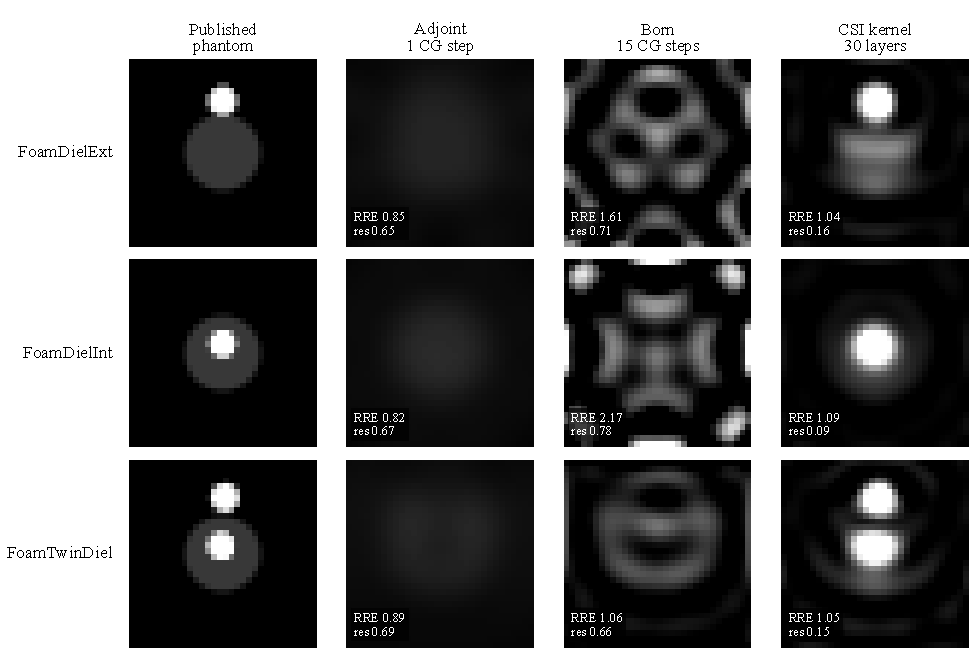
\includegraphics[width=\linewidth]{figures/fig_fresnel_recon.pdf}
\caption{Measured-data reconstruction at $3\,\mathrm{GHz}$, one row per published phantom. The
columns are an algorithmic ladder computed on the same measured field, calibration constant,
projection box and CG solve: the published phantom, a one-CG-step adjoint, a $15$-CG-step Born
solve at the incident field, and the $30$-layer contrast-source kernel. All panels share one grey scale
$[0,1]$, so the adjoint column is not empty but strongly shrunk
($\max|\chi|\le\numv{\NumFrBaseDsmPeakHi}$). Corner values are the relative error and the
label-free data residual.}
\label{fig:fresnelrecon}
\end{figure}

Table~\ref{tab:fresnelrecon} and Fig.~\ref{fig:fresnelrecon} report the result. The
recovered residual $r_{\mathrm{net}}$ lies between $0.07$ and $0.50$, against the
model-to-instrument floor $r_{\mathrm{true}}$ between $0.09$ and $0.12$; in two of the
nine instances (FoamDielInt at $3$ and $4\,\mathrm{GHz}$) the recovered residual is
\emph{below} the published phantom's own fit, and in the worst case (FoamTwinDiel at
$4\,\mathrm{GHz}$) it is within a factor of about $4.7$ of that floor. The image confirms
this quantitatively: the single and twin cylinders are localised, the bright plastic
inclusions and the weaker foam host are separated by contrast, and the worst case is the
three-cylinder twin phantom at the highest frequency. Throughout the rollout the contrast
source stays at $\max\|w\|_\infty\in[0.04,0.09]$, and $\max|\chi|$ reaches the upper box
edge $2.5$ where the plastic cylinder saturates the box. The a-priori weak-scattering
hypothesis $\beta_0=\chi_{\max}\norm{\mathbf{G}_b}_2<1$ does \emph{not} hold on this
$2\lambda$ domain, as Sec.~\ref{sec:fresnel} already reported; the boundedness observed
here is therefore the \emph{measured} boundedness of the actual rollout, not a consequence
of the field-subsystem contraction certificate. The projection is what converts that
measured boundedness into a hard box; in the tested instances removing the projection does
not, by itself, produce divergence within the horizon, so the observed boundedness is not
by itself evidence that the projection is necessary.

The ladder in Fig.~\ref{fig:fresnelrecon} is the check that the earlier version of this figure
could not support, and it does not flatter the kernel. The adjoint image has the smallest
relative error of the three reconstructions ($\numv{\NumFrBaseDsmRreLo}$--$\numv{\NumFrBaseDsmRreHi}$)
and the $30$-layer kernel the largest
($\numv{\NumFrKernRreLo}$--$\numv{\NumFrKernRreHi}$); the ordering reverses on the label-free
data residual ($\numv{\NumFrBaseDsmResLo}$--$\numv{\NumFrBaseDsmResHi}$ for the adjoint against
$\numv{\NumFrKernResLo}$--$\numv{\NumFrKernResHi}$ for the kernel) and on the image itself, since
the adjoint contrast peaks at $\numv{\NumFrBaseDsmPeakHi}$ against a box edge of $2.5$. A
pixel-wise $\ell_2$ metric rewards a shrunk image, which is the same mechanism that makes the
constrained arm of Fig.~\ref{fig:images} the larger number there; the residual is the quantity
that says whether an image explains the measurement at all. The two linearised solves bracket
this behaviour ($\numv{\NumFrBaseBornRreLo}$--$\numv{\NumFrBaseBornRreHi}$, residual up to
$\numv{\NumFrBaseBornResHi}$), so what separates the kernel column from the Born column is the
nonlinear iteration and not the linear solve. One negative result belongs here as well: at
$3\,\mathrm{GHz}$ the step search returned the canonical pair
$(\alpha,\gamma)=(0.5,0.5)$ for all three phantoms, so the kernel column \emph{is} the archived
reconstruction and the search adds nothing on these measured cases; we report that rather than
retune it.

We additionally attempted a direct zero-shot transfer of the trained correction
networks by aligning the receiver count with the trained checkpoint. The transferred run
collapses to a near-zero output because the trained feature map expects the synthetic point
spread and fixed receiver Green block, whereas the measured geometry has a per-view arc and a
different field normalisation. The boundedness certificate depends only on
$\mathbf{G}_b,\mathbf{G}_s$ and the projection set, not on the correction weights; the
collapse therefore confirms that the certificate transfers across geometries while the trained
feature map does not.

\section{Discussion and Limitations}\label{sec:lim}
Our results certify a \emph{regime}, not every regime, and several findings are negative.

\noindent\textbf{(i)} Per-layer Euclidean contraction is impossible on $\alpha>\alpha_c$ by Prop.~\ref{prop:imposs}, with the
threshold $\alpha_c=(\theta\mathcal{E})^{-1}$ measured here as $\numv{\NumAlphaC}$; and the geometric
bounds that would follow from contraction, the drift radius $\bar\epsilon/(1-\rho_\chi)$ and the
noise gain $\Lambda/(1-\rho)$, are therefore \emph{conditional}, and the hypotheses are not all
discharged by our measurements: $\sigma_{\max}=\numv{\NumPhysSigma}>1$ holds, while $\rho_\chi<1$
is refuted in the unconstrained arm and left undecided in the constrained one. We report the
measured quantities instead, and we would regard quoting either radius without its hypothesis as a
misrepresentation of what this theory proves.
(ii) The a-priori field certificate requires $\beta_0=\chi_{\max}\norm{\mathbf{G}_b}_2<1$. Outside it
(strong scatterers) the projection and the exact accounting remain meaningful but the contraction
statements lose their hypotheses.
(iii) The amplitude and slope budgets do not improve measured accuracy or measured noise robustness
in our setting; their contribution is that every trained network carries explicit, recomputable
constants. We therefore do not report budgeted architectures as accuracy improvements.
(iv) The projection is a load-bearing element for boundedness but is only \emph{nonexpansive}, not
contractive: it cannot by itself create a fixed point, only prevent escape and supply a known
constant. Networks whose physics core is not contracting in the field variable (strong contrast)
would need the averaged operator construction of Remark~\ref{rem:averaged}, at the accuracy cost
identified in Proposition~\ref{prop:tri}.
(v) Our ablations also show the limits of ablation-based reasoning: a network retrained without
the projection looks fine at $800$ layers, and only the frozen-weight test, reported in Table~\ref{tab:abl2}, reveals that the same weights collapse when the projection is removed.
Boundedness observed after joint retraining is not evidence that the guard is unnecessary.
(vi) The experiments are 2-D and moderately sized. The theory, however, is dimension-free, and
every certified quantity in Table~\ref{tab:cert} is computed from quantities a practitioner can
recompute for any grid, aperture or contrast distribution, \emph{provided the certified
hypotheses are checked at that operating point}, because at our own operating point they are not
all satisfied: $\beta_0<1$ for the field certificate of Thm.~\ref{thm:field}, an admissible contrast box for the
invariance of Thm.~\ref{thm:bounded}, and the amplitude/slope budgets of \eqref{eq:budgets} for the
correction $H_k$. A certificate is only as good as that check. Two modelling restrictions also lie
outside the theory as stated. First, the contrast is taken \emph{real and non-negative}, as it is for passive lossless dielectrics, which is what makes $\Pi_{[0,\chi_{\max}]}$ an admissible physics prior; for
lossy or active media the contrast is complex and the projection has no counterpart as written; an
analogous certificate would require a complex admissible set with its own constant.
Second, $\beta_0$ depends on $\norm{\mathbf{G}_b}_2$ and therefore on the discretisation, so the
field certificate is stated for the discretisation actually used, not for the continuous problem.
The recomputation at $64\times64$ and $128\times128$ cells of Sec.~\ref{sec:grid} keeps
$\beta_0<1$ and moves the operator-level quantities by less than $1\%$, but the certificate
remains a discretisation-level object, and that is the scope of the statement.
(vii) The learned corrections improve conditioning and speed but not the information content: the
noise-sensitivity floor is set by the measurement operator.
(viii) The impossibility proposition is stated per operating point: $\alpha_c$ depends on
$\mathcal{E}=\max_r\norm{E_{\cdot,r}}_2$, which varies across the test set and along the rollout. We have reported it at the
measured operating points used for Table~\ref{tab:cert} and swept it in Fig.~\ref{fig:alphac};
a distribution-free version would require a lower bound on the field concentration, which we do not
have and do not claim.
(ix) The accuracy comparison of Sec.~\ref{sec:exp} is an \emph{iteration-count} comparison against
the damped alternating fixed-point iteration at matched per-layer cost, not a wall-clock comparison
against an established classical solver. We quantify the per-layer surcharge of the learned
module ($1{+}\numv{\NumCostLayerOverhead}$ in median wall-clock, $\numv{\NumCostLayerOverheadPct}\%$
over a classical layer, on the production shapes at batch $16$) so that the iteration reduction can
be discounted by the reader, but we do not claim that the $12\times$ iteration reduction translates
into a $12\times$ wall-clock reduction. We now also run two stronger classical references, 
contrast source inversion and the subspace-based optimization method, and they too remain above
the unrolled networks: at matched depth the margin against SOM is
$\numv{\NumSomMargKEight}$, whereas the best-vs-best margin $\numv{\NumSomMargBest}$ lies within
the re-run floor. The comparison is therefore not an artefact of a weak baseline, and it is not
claimed as a win at matched budget either.
(x) The contrast step is evaluated by a fixed $n_{\mathrm{cg}}=\numv{\NumNCg}$-step conjugate-gradient
loop, not a converged solve. The certified blocks $C$ and $D$ are closed-form and free of the solver,
so the impossibility and boundedness statements are unaffected; but the contrast-path Jacobian blocks
$A$, $B$ and the full layer norm \emph{are} solver-resolution dependent, and we report them at both
the implemented and a converged setting rather than quoting one, with the
directional-derivative control that pins the effect and a systematic $n_{\mathrm{cg}}$ sweep that
measures it. Any contrast-path quantity a reader recomputes should be
compared at matched solver resolution.
(xi) The study is theory plus simulation on synthetic 2-D TM data, extended by the
operator-level Fresnel recomputation of Sec.~\ref{sec:fresnel} and the measured-field
reconstruction of Sec.~\ref{sec:fresnelrecon}. The operator-level recomputation uses our
own forward solve on the published geometry at one frequency and one target; the
measured reconstruction uses the real scattered fields of three dielectric phantoms at
three inside-ROI frequencies but runs the classical layer structure without the trained
correction weights, because those weights expect the training point spread. In two of the
nine measured instances the recovered residual is at or below the published phantom's own
fit; the remaining instances are within a factor of about $4$ of that floor. A direct
zero-shot transfer of the trained weights was attempted and collapsed to the near-zero
image, so a geometry-adapted transfer remains future work.

(xii) The empirical generalization conclusions of Sec.~\ref{sec:exp} are drawn from synthetic data with $\chi\in[0.25,0.5]$ on a single $32\times32$ grid. The cross-contrast boundary is measured in Sec.~\ref{sec:contrast} and the cross-geometry behaviour in Sec.~\ref{sec:geom}: the field-subsystem certificate $\beta_0<1$ holds only at $\chi_{\max}=\numv{\NumMaxChiBox}$ and fails at every raised ceiling, where the projection alone keeps the states bounded and the estimate degrades by truncation rather than by instability; across four structurally distinct geometry families the reconstruction error stays within a modest band and projection boundedness holds unconditionally at depth $100$. The shared contrast range and grid resolution remain scope limits; the measured-field
reconstruction of Sec.~\ref{sec:fresnelrecon} uses the classical layer without the trained
weights.

\section{Conclusion}
We set out to state what can be guaranteed for an unrolled Born/contrast-source network, and the
answer has a definite shape. The $\chi\!\to\!w$ block of the layer Jacobian is exactly
$\theta\alpha\,\mathrm{diag}(E)$, so for $\alpha>\alpha_c=(\theta\mathcal{E})^{-1}$ and for
\emph{every} learned correction the composite is provably non-contractive, and the obstruction sits
in a channel that a correction applied to the contrast alone cannot reach. That is a property of the
architecture, not of the data, the loss or the training schedule.

What survives is layer-wise. A field-subsystem contraction
$\beta_0=\chi_{\max}\norm{\mathbf{G}_b}_2$ holds for every step size at which it holds at all; an
invariant compact set is certified for arbitrary depth under a nonexpansive physics-prior projection;
the finite-depth noise propagation is accounted exactly, including the non-normal factor that a
geometric series omits; and the two geometric statements are labelled conditional because their
hypotheses are not discharged at our operating point. The checks have an order: $\beta_0$ on the
actual discretisation before training, the projection and the trunk bound during it, and a
re-measured $(\sigma_{\max}(J),\rho,M_J,\Lambda)$ at every new operating point. The cost of the
constants is measured rather than argued: at matched depth the constrained family is
$\numv{\NumPriceDelta}$ worse in test-set relative reconstruction error than the unconstrained one,
and what the gap buys is a constant that can be recomputed, not a rate that can be assumed.

The scope limits are part of the result. Every certificate is conditional on the discretisation,
the aperture, the contrast box and the operating point; on the published Fresnel geometry
$\beta_0=\numv{\NumFresnelBeta}$, so no a-priori field certificate is available there and
boundedness is what remains; and the $\chi$-map Lipschitz constant that the drift radius needs is
neither refuted nor verified by the proxies we could measure, which is why that radius stays
conditional. Nothing here proves that a trained network converges: no fixed point is shown to
exist, to be unique or to be attracting, and no unconditional noise gain is claimed; the two
statements that are proved concern the field subsystem and the invariant set, and they are the
whole of the a-priori content. Carrying the certificate to a kernel whose field step is not the Born/contrast-source
one, and discharging the $\chi$-map hypothesis instead of bounding it, are the two directions in
which the boundary now moves.

\noindent\textbf{Statement of Novelty.}
(1) We prove that the Born/contrast-source unrolled layer is provably non-contractive above an
explicit step-size threshold, because the bilinear coupling block is exactly
$\theta\alpha\,\mathrm{diag}(E)$; this obstruction has not been identified in prior unrolling
work. (2) We supply a layer-wise certification framework: a field-subsystem contraction condition
$\beta_0<1$, an invariant compact set under a nonexpansive contrast projection, and an exact
finite-depth noise account that exposes the non-normal factor a naive geometric sum omits.

\noindent\textbf{(3)} We delimit what is and is not certified: the geometric radii are conditional and the
$\rho_\chi$ contraction hypothesis is measured to fail at the operating point, so we report
measured bounds rather than advertising guarantees. (4) The framework is validated on synthetic
2-D TM scattering with four baselines and on the published Institut Fresnel measured geometry.

\acknowledgement{During the preparation of this manuscript, the authors used DeepSeek-V4.1-Flash, an AI-assisted writing tool, for language polishing, LaTeX formatting support, and generating figures from numerical data supplied by the authors. The authors have reviewed and edited all content and take full responsibility for the publication.}

\funding{This research was supported by the Science and Technology Research Project of Henan Province, China, under Grant Nos.\ 262102210030 and 242102321138.}

\authorcontributions{The authors confirm contribution to the paper as follows: conceptualization, Longgang Wang; methodology, Longgang Wang; software, Guoqiang Wang; validation, Guoqiang Wang and Nianfeng Shi; formal analysis, Longgang Wang; investigation, Guoqiang Wang and Nianfeng Shi; resources, Nianfeng Shi; data curation, Guoqiang Wang; writing---original draft preparation, Longgang Wang; writing---review and editing, Longgang Wang and Guoqiang Wang; visualization, Guoqiang Wang; supervision, Longgang Wang; project administration, Longgang Wang; funding acquisition, Longgang Wang. All authors reviewed and approved the final version of the manuscript.}

\availabilityofdataandmaterials{The code and numerical logs that support the findings of this study are openly available in the GitHub repository at \url{https://github.com/jiumi01/unrolled-inverse-scattering} (tag v1.2). The measured Institut Fresnel data set is available from the Institut Fresnel website.}

\ethicsapproval{Not applicable. The study involves no human participants, human tissue or animals; the measured fields used in Sec.~\ref{sec:fresnelrecon} are a public scattering database.}

\conflictsofinterest{The authors declare no conflict of interest.}

\clearpage
\abbreviations{Abbreviations}{\indent The following abbreviations are used in this manuscript:\\
\footnotesize\begin{tabular}{@{}ll@{}}
2-D & two-dimensional\\
CG & conjugate gradient\\
CIE & contraction (compressed) integral equation\\
CSI & contrast source inversion\\
GMRES & generalised minimal residual method\\
ISP & inverse scattering problem\\
LS & Lippmann--Schwinger\\
MoM & method of moments\\
NBIM & Neural Born Iterative Method\\
RRE & relative reconstruction error\\
SNR & signal-to-noise ratio\\
SOM & subspace-based optimization method\\
TM & transverse magnetic
\end{tabular}}

\reftitle{References}
\begin{thebibliography}{99}
\bibitem{born_lit}
Habashy TM, Groom RW, Spies BR. Beyond the Born and Rytov approximations: A nonlinear approach to electromagnetic scattering. J Geophys Res. 1993;98(B2):1759--1775.
\bibitem{csi_lit}
van den Berg PM, Kleinman RE. A contrast source inversion method. Inverse Probl. 1997;13(6):1607--1620.
\bibitem{som_lit}
Chen X. Subspace-based optimization method for solving inverse-scattering problems. IEEE Trans Geosci Remote Sens. 2010;48(1):42--49.
\bibitem{somnet}
Liu Y, Zhao H, Song R, Chen X, Li C, Chen X. SOM-Net: Unrolling the subspace-based optimization for solving full-wave inverse scattering problems. IEEE Trans Geosci Remote Sens. 2022;60:2007715.
\bibitem{unrolledcnn}
Zhang Y, Lambert M, Fraysse A, Lesselier D. Unrolled convolutional neural network for full-wave inverse scattering. IEEE Trans Antennas Propag. 2023;71(1):947--956.
\bibitem{neuralbim}
Shan T, Lin Z, Song X, Li M, Yang F, Xu S. Neural Born iterative method for solving inverse scattering problems: 2D cases. IEEE Trans Antennas Propag. 2023;71(1):818--829.
\bibitem{deepnis}
Li L, Wang LG, Teixeira FL, Liu C, Nehorai A, Cui TJ. DeepNIS: Deep neural network for nonlinear electromagnetic inverse scattering. IEEE Trans Antennas Propag. 2019;67(3):1819--1825.
\bibitem{mfneuralbim}
Liu D, Shan T, Li M, Yang F, Xu S. Multi-frequency neural Born iterative method for solving 2-D inverse scattering problems. IEEE Trans Comput Imaging. 2025;11:1243--1257.
\bibitem{ciesomnet}
Xu K, et al. Physically unrolling network under contraction integral equation for limited-aperture inverse scattering problem. IEEE Trans Antennas Propag. 2023;71(11):9130--9135.
\bibitem{kernelunroll}
Li X, Zhang T, Bi D, Peng L, Xie Y. Kernelized deep unfolding network with joint physical constraints for electromagnetic inverse scattering imaging. IEEE Trans Antennas Propag. 2026;74(2):1707--1722.
\bibitem{li2019cnn}
Li L, Wang LG, Teixeira FL. Performance analysis and dynamic evolution of deep convolutional neural network for electromagnetic inverse scattering. IEEE Antennas Wireless Propag Lett. 2019;18(11):2259--2263.
\bibitem{lista}
Gregor K, LeCun Y. Learning fast approximations of sparse coding. In: Proc ICML; 2010. p. 399--406.
\bibitem{listacp}
Chen X, Liu J, Wang Z, Yin W. Theoretical linear convergence of unfolded ISTA and its practical weights and thresholds. In: Proc NeurIPS; 2018.
\bibitem{alista}
Liu J, Chen X, Wang Z, Yin W. ALISTA: Analytic weights are as good as learned weights in LISTA. In: Proc ICLR; 2019.
\bibitem{cui_reg}
Cui ZX, Zhu Q, Cheng J, Zhang B, Liang D. Deep unfolding as iterative regularization for imaging inverse problems. Inverse Probl. 2024;40(2):025011.
\bibitem{sherry_nonexp}
Sherry F, Celledoni E, Ehrhardt MJ, Murari D, Owren B, Sch\"onlieb CB. Designing stable neural networks using convex analysis and ODEs. Physica D. 2024;463:134159.
\bibitem{mondeq}
Winston E, Kolter JZ. Monotone operator equilibrium networks. In: Proc NeurIPS; 2020.
\bibitem{algomapping}
Tay DB. On iterative algorithms with different mapping in each iteration. Algorithms. 2026;19(6):470.
\bibitem{mukherjee2023}
Mukherjee S, Hauptmann A, \"Oktem O, Pereyra M, Sch\"onlieb CB. Learned reconstruction methods with convergence guarantees: A survey of concepts and applications. IEEE Signal Process Mag. 2023;40(1):164--182.
\bibitem{monga_survey}
Monga V, Li Y, Eldar YC. Algorithm unrolling: Interpretable, efficient deep learning for signal and image processing. IEEE Signal Process Mag. 2021;38(2):18--44.
\bibitem{convergentborn}
Kleinman RE, Roach GF, van den Berg PM. Convergent Born series for large refractive indices. J Opt Soc Am A. 1990;7(5):890--897.
\bibitem{cie_lit}
Isernia T, Crocco L, D'Urso M. New tools and series for forward and inverse scattering problems in lossy media. IEEE Geosci Remote Sens Lett. 2004;1(4):327--331.
\bibitem{kleinvandenberg}
Kleinman RE, van den Berg PM. Iterative methods for solving integral equations. Prog Electromagn Res. 1991;5:67--102.
\bibitem{slaney}
Slaney M, Kak AC, Larsen LE. Limitations of imaging with first-order diffraction tomography. IEEE Trans Microw Theory Tech. 1984;32(8):860--874.
\bibitem{devalle2023}
de Valle C, Centofanti E, Chouzenoux E, Pesquet JC. Stability of unfolded forward-backward to perturbations in observed data. In: Proc 31st Eur Signal Process Conf (EUSIPCO); 2023. p. 865--869.
\bibitem{fresnel_db}
Belkebir K, Saillard M. Special section: Testing inversion algorithms against experimental data. Inverse Probl. 2001;17(6):1565--1571; Geffrin JM, Sabouroux P, Eyraud C. Free space experimental scattering database continuation: experimental set-up and measurement precision. Inverse Probl. 2005;21(6):S117--S130.
\end{thebibliography}
\end{document}